
\section{Données}
%%%%%%%%%%%%%%%%%%%%%%%%%%%%%%%%%%%%%%%%%%%%%%%%%%%%%%%%%%%%%%%%%%%%%%%
\subsection{Présentation}

Nous disposons de deux séries de données contenues dans le package \lstinline!gumbel! correspondant à la vitesse maximale du vent par jour, sur la période août 2005 - avril 2007,
relevée à deux stations différentes en région Rhône-Alpes : l'une à Saint-Martin-en-Haut (département du Rhône) et et une autre à Echirolles (département de l'Isère).

~\\~
Notons :
\begin{itemize}
\item $(X_t)_t$ la série relative à la force maximale du vent (en m/s) par jour relevée par la station à Saint-Martin-en-Haut 
\item $(Y_t)_t$ la série relative à la force maximale du vent (en m/s) par jour relevée par la station à Echirolles.
\end{itemize}

~\\~
Puisque les jeux de données appelés dans $R$ \lstinline!windEchirolles! et \lstinline!windStMartin! possèdent 
un nombre d’enregistrements différents en 2007, nous sélectionnons le plus petit sous-ensemble. Les données manquantes sont aussi retirées de la série.

Nous avons ainsi deux vecteurs de données contenant chacun $n=633$ données (correspondant à 633 jours).


\subsection{Formalisation}

Nous allons donc nous intéresser à la relation existant entre ces deux variables aléatoires réelles au moyen de modélisations par copules.
En effet,  les fonctions copules permettent de déterminer la nature de dépendance des séries qu’elle soit linéaire ou pas, monotone ou pas.

D'une manière explicite, les copules sont des fonctions de répartition particulières,
qui lient les fonctions de répartition multivariéees de lois de probabilitée dans $\mathbb{R}^d$, où $d \geq 2$ (ici $d$ sera égal à 2 car nous aurons un modèle bivarié) aux fonctions de répartition marginales de leurs coordonnées. 
La caractéristique des copules permet de séparer les distributions marginales de la structure de dépendance.

Plus précisément, $X$ et $Y$  sont définies sur un espace de probabilité $(\Omega,\mathcal{A},\mathbb{P})$, de fonction de répartition conjointe $H$ et de marginales $F$ et $G$.

D'après Sklar (1959), il existe une fonction de répartition bivariée $C$ dont les marges sont uniformes sur $[0,1]$, telle que :
$$
H(x,y) = C(F(x),G(y))
$$

De plus, si $F$ et $G$ sont continues, la copule $C$ est alors unique et on a :

$$
\forall (u,v) \in [0,1]^2 ~~ C(u,v) = H(F^{-1}(u),G^{-1}(v))
$$

En fait, il s'agit de la loi du couple $(U,V) = (F(X),G(Y))$.

Nous allons donc chercher la copule qui s’adapte le mieux à nos données.




\subsection{Observation graphique}

Il est maintenant temps de considérer la structure empirique des échantillons. Avant de tracer les diagrammes représentatifs de 
la dépendance des données, nous allons exposer quelques notions.


\subsubsection{Fonctions de répartition empiriques}

Le cadre général de l’estimation non paramétrique des loi marginales $F$ et $G$ s’appuie sur les fonctions de répartition empiriques, définies par :

$$
F_n(x) = \frac{1}{n} \sum_{i=1}^n \mathbb{1}_{x_i \leq x}
\text{~~~~et~~~~}
G_n(x) = \frac{1}{n} \sum_{i=1}^n \mathbb{1}_{y_i \leq y}
$$

pour un n-échantillon de la loi $F$ et n-échantillon de la loi $G$.

Ainsi, nous noterons respectivement $F_n$ et $G_n$ les fonctions de répartion empiriques des marginales $F$ et $G$.


\subsubsection{Scatter plot et Rank-rank plot}

Nous allons tout d'abord déterminer le dépendogramme relatif à nos données.
Il représente la structure de dépendance sous la forme d'un nuage de points des marges uniformes $(u,v)$ extraites de l'échantillon.

En d'autres termes, il s'agit tout simplement d'un scatter plot faisant figurer les marges empiriques relatives à l'échantillon
$(y_i )_i$ en fonction des marges empiriques relatives à l'échantillon $(x_i)_i$, soit le scatter plot des points suivants $(\hat{u},\hat{v})$.
Ces marges uniformes sont définies par les statistiques de rang issues de l'échantillon. C'est-à-dire, pour tous les $\hat{u}, \hat{v}$, nous utilisons 
les fonctions de répartition empiriques $F_n$ et $G_n$ calculées en $x_i$ et $y_i$ respectivement.

Par définition d'une marge uniforme, on a $F(x) = u$ et donc : 


Pour $1\leq i \leq 1$,
$$
\widehat{u_i} = F_n(x_i) = \frac{1}{n} \sum_{k=1}^n \mathbb{1}_{x_k \leq x_i}
$$

De la même manière, on a :

Pour $1\leq i \leq 1$,
$$
\widehat{v_i} = G_n(y_i) = \frac{1}{n} \sum_{k=1}^n \mathbb{1}_{y_k \leq y_i}
$$

Autrement écrit, cela revient à poser :

$$
\widehat{u_i} = \frac{r_i}{n} \text{~~~~et~~~~} \widehat{v_i} = \frac{s_i}{n}
$$
où $r_i$ est le rang de $x_i$ parmi $x_1,...,x_n$ et $s_i$ est le rang de $y_i$ parmi $y_1,...,y_n$ .

\underline{Remarque} : par la suite et par souci de simplification des notations, nous noterons les estimations des marginales $\widehat{u}$ 
et $\widehat{v}$ : $u$ et $v$.

Nous traçons donc le diagramme de dispersion des points $(x_i,y_i)_{1\leq i \leq n}$ (en anglais "scatter plot") et 
le dépendogramme (ou graphique des rangs, ou en anglais "rank-rank plot"), graphique des points $\left( \frac{r_i}{n}, \frac{s_i}{n}\right)_{1\leq i \leq n}$.

\noindent%
\begin{figure}[H]
    \begin{center}
      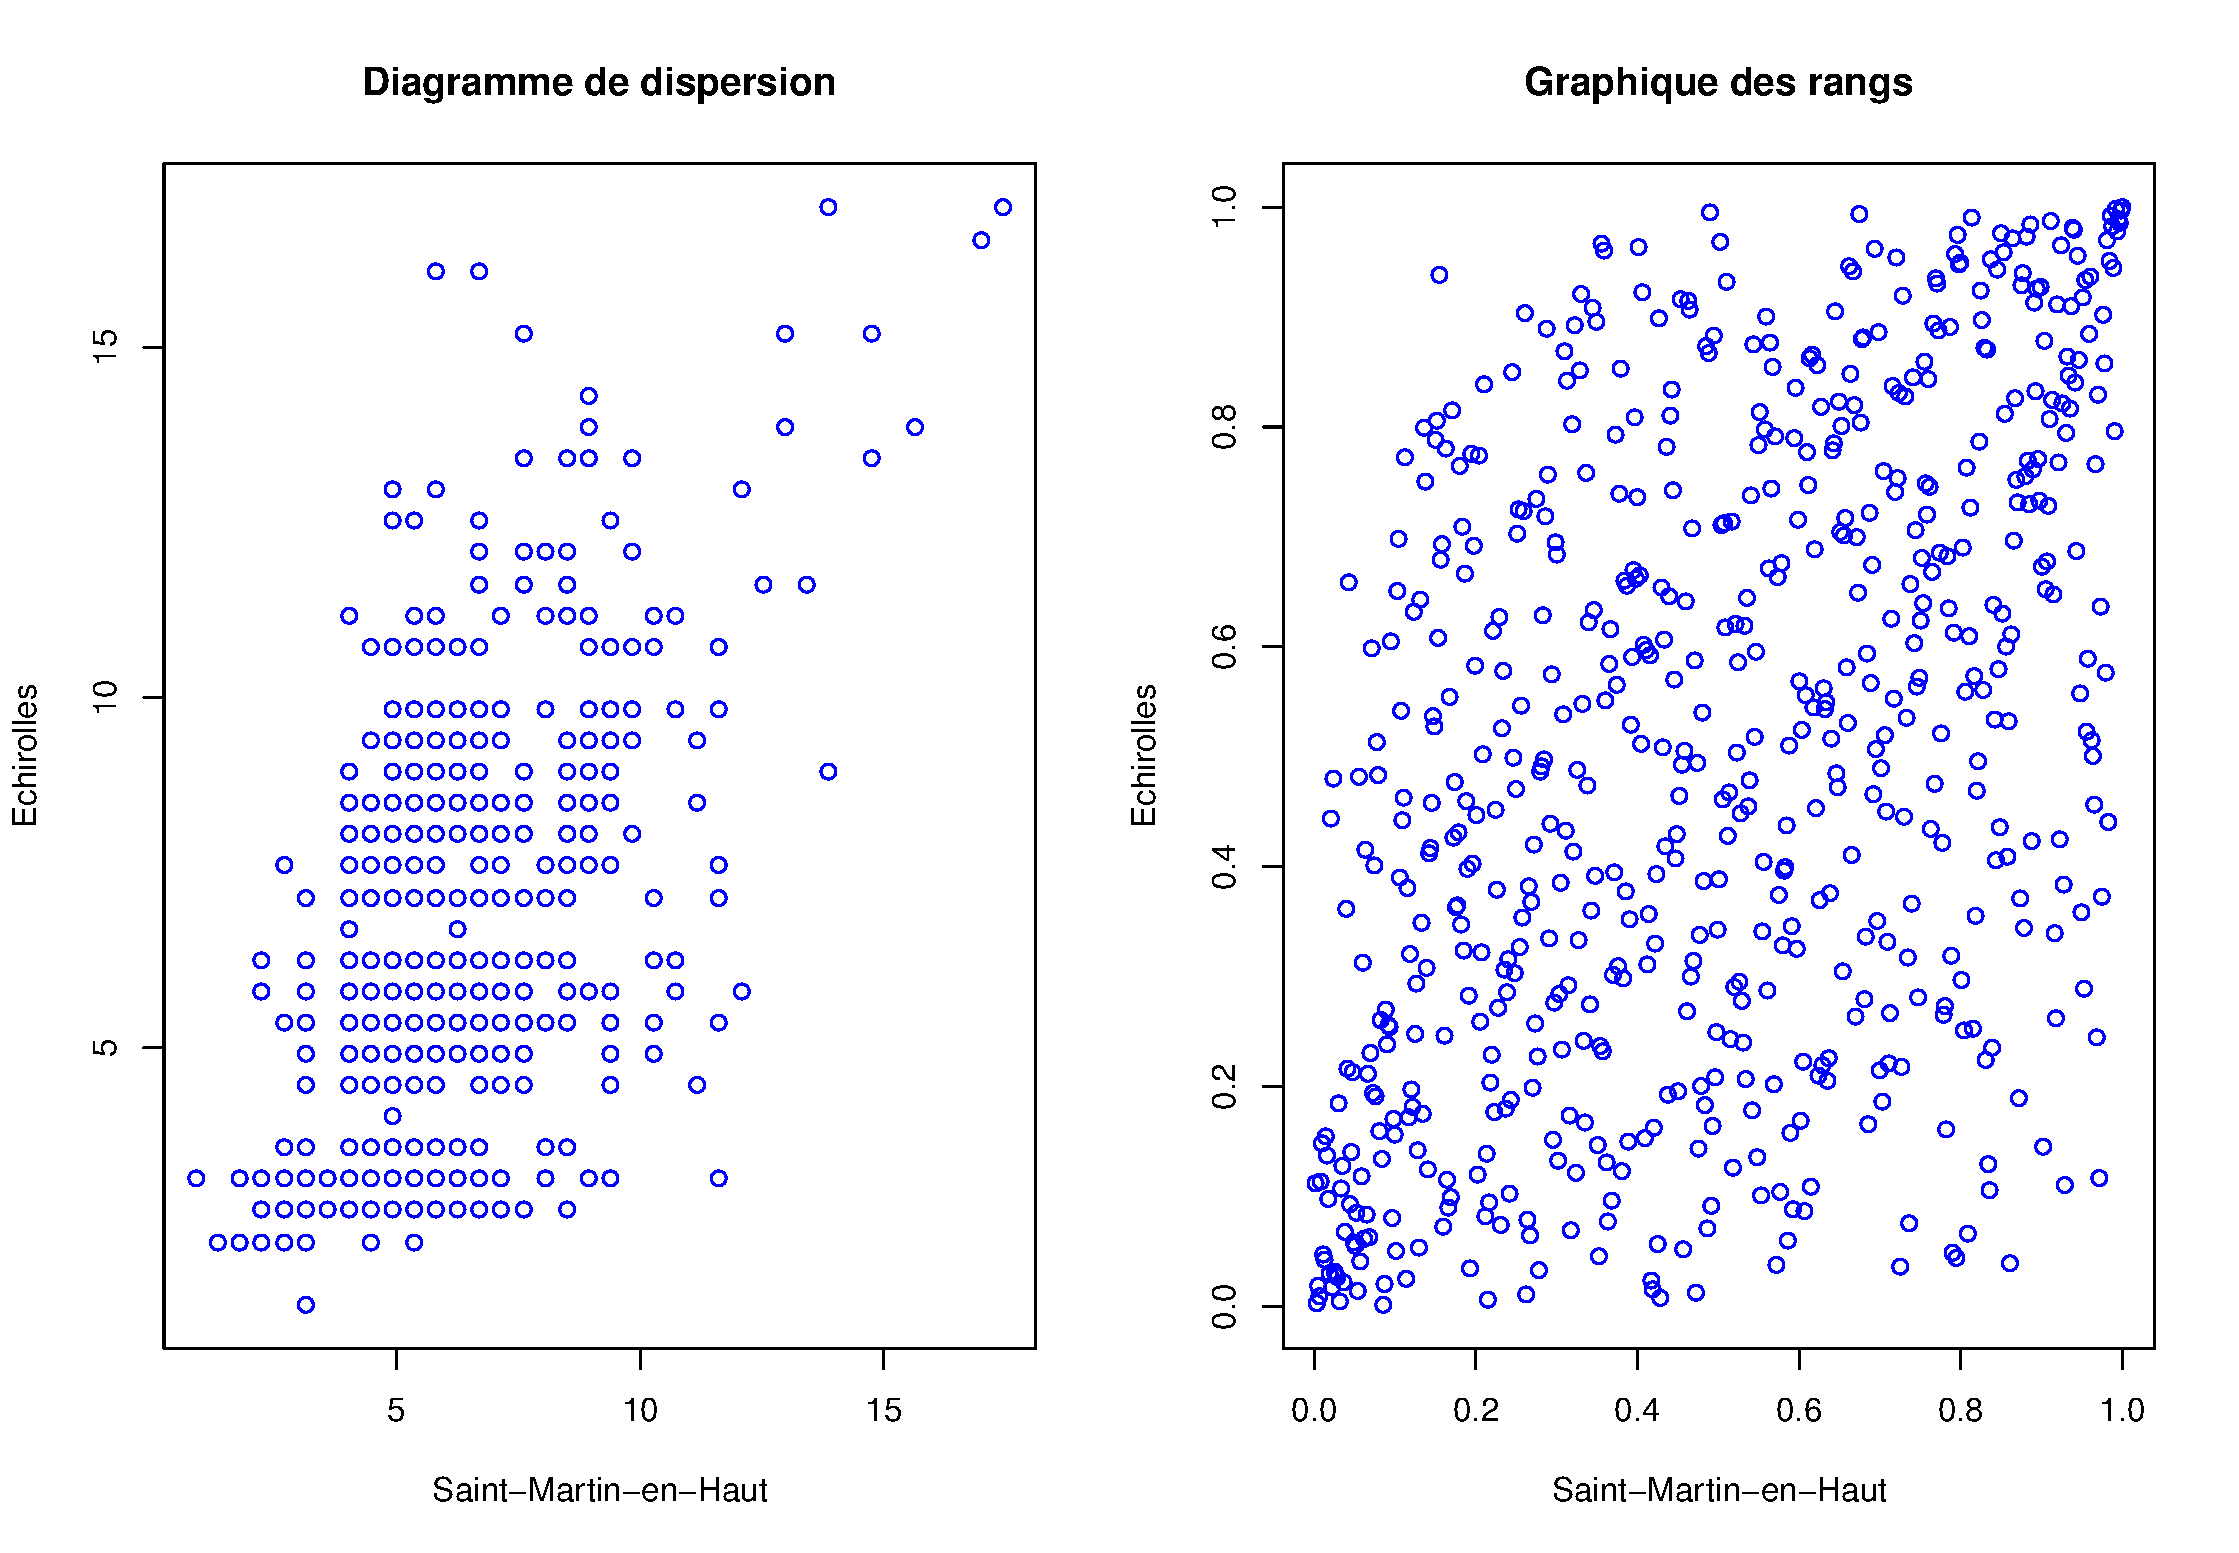
\includegraphics[width=17 cm, angle=0]{./pictures/scatter_et_rankrank.png}
      \centering\caption{Diagramme de dispersion et graphique des rangs}
    \end{center}
\end{figure}

Au vu du dépendogramme, il semble que les dépendances entre les forces du vent relevées par les deux stations sur la période d'étude soit positive mais modérée. 
En effet, le dépendogramme a une forme d'ellipse dont le grand axe serait dans la direction de la première bissectrice.
On observe un regroupement de points sur la queue à gauche et un regroupement de points sur la queue à droite. On peut donc supposer qu'il y ait une dépendance de queue à gauche 
et à droite. Cependant, cette approche restant limitée, on ne se limitera pas à l'étude des modèles de copules présentant cette seule caractéristique mais à un ensemble de copules
pouvant représenter cette dépendance positive, sur la queue supérieure et/ou inférieure de la distribution.

Nous allons dès à présent nous intéresser à la mesure de cette dépendance. 

\subsection{Mesurer la dépendance}

\subsubsection{Dépendance ou corrélation ?}

Il est important de rappeler que les notions de dépendance et de corrélation sont différentes.
En effet, si $X$ et $Y$ sont indépendantes, cela implique que $X$ et $Y$ sont non corrélées. Mais attention, la réciproque est fausse, sauf dans
le cas où les variables sont gaussiennes car la dépendance est alors entièrement caractérisées par le coefficient de corrélation.

Un contre-exemple permettant d'illustrer cette remarque est le suivant :

Soit $X \sim \mathcal{N}(0,1)$ et $Y = X^2$, alors $\operatorname{Cov}(X,Y) = E[X^3] = 0$.

Le coefficient de corrélation doit donc être utilisée avec précaution car il n’est pertinent qu’en présence de distributions elliptiques (distribution multivariée
Normale ou de Student) ou de dépendance linéaire.


\subsubsection{Corrélation de Pearson}

Le coefficient de corrélation linéaire de Pearson est défini, pour nos deux variables aléatoires $X$ et $Y$ de variances finies, par :

$$
\rho(X,Y) = \frac{\operatorname{Cov}(X,Y)}{\sqrt{ \operatorname{Var}(X) \operatorname{Var}(Y)}}
$$

où $\operatorname{Cov}(X,Y) = E[XY] - E[X] E[Y]$ est la covariance entre $X$ et $Y$ et $\operatorname{Var}(X)$, $\operatorname{Var}(Y)$ correspondent aux variances respectives
de $X$ et $Y$.

On a alors :

\begin{itemize}
\item $X$ et $Y$ sont corrélées linéairement $\Longleftrightarrow \rho(X,Y) \neq 0$
\item $X$ et $Y$ sont non corrélées linéairement $\Longleftrightarrow \rho(X,Y) = 0$
\end{itemize}

Le coefficient de corrélation de Pearson est la mesure la plus connue. Mais il constitue une mesure très imparfaite de la dépendance. Il ne
peut se mettre sous une forme ne faisant intervenir que la copule, les marginales restent présentent dans l’expression : ce coefficient n’est donc
pas une mesure de dépendance.

De plus, il n’intègre que la composante linéaire de la dépendance, au sens où $r(X,Y) \pm 1$ si et seulement si $Y= a \times x + b$.

Enfin, on peut montrer (en utilisant l'inégalité de Tchen) que, pour les marginales fixées, toutes les valeurs
comprises entre -1 et +1 ne sont pas atteignables.

Ainsi, on retiendra que ce coefficient :

\begin{itemize}
\item mesure mal une association non-linéaire,
\item est trop sensible aux valeurs extrêmes,
\item ne mesure pas vraiment la distance à l'indépendance,
\item n'est pas toujours défini (Cauchy par exemple).
\end{itemize}

Pour nos deux échantillons de données, on obtient la valeur suivante pour le coefficient de Pearson :

\begin{center}
\fbox{$\rho(X,Y) = 0,524 $}
\end{center}

Cette valeur positive laisse à penser, conformément au dépendogramme, que les relevés de la station d'Echirolles et ceux de la station de Saint-Martin-en-Haut ont une dépendance positive. Mais ce resultat reste relativement peu fiable pour les raisons citées, principalement par le fait que les variables d'intérêt présentent une dépendance non linéaire.


Pour remédier à cela, nous avons recours à d’autres indicateurs de dépendance se basant sur les rangs et les concordances observés de notre échantillon de données. 
Ainsi, nous utilisons des coefficients de corrélation non linéaires, comme le rhô de Spearman ou le tau de Kendall.

\subsubsection{Rhô de Spearman}

Le rhô de Spearman $\rho_S$ se définit comme la corrélation entre les rangs d'observations.

Soient $X=(X_1,...,X_n)$ et $Y=(Y_1,...,Y_n)$ deux vecteurs aléatoires réels et $R = (R_1,...,R_n)$ et $S = (S_1,...,S_n)$ les vecteurs aléatoires des rangs respectivement
de $X$ et $Y$, alors :

$$
\rho_s = \rho(R,S) = \frac{\operatorname{Cov}(R,S)}{\sqrt{ \operatorname{Var}(R) \operatorname{Var}(S)}} = \frac{ \sum_{i=1}^n (R_i - \bar{R}) \times (S_i - \bar{S})  }{ \sqrt{   \sum_{i=1}^n (R_i - \bar{R})^2 \times  \sum_{i=1}^n (S_i - \bar{S})^2    }    }
$$

De plus, $rho_s$ vérifie les propriétés suivantes :

\begin{enumerate}

\item $\rho_s(X,Y) = \rho_s(Y,X), ~~\forall (X,Y)$
\item $|\rho_s(X,Y)| \leq 1, ~~\forall (X,Y)$
\item 
\begin{itemize}
\item $X$ et $Y$ comonotones $\Longleftrightarrow \rho_s(X,Y)=1$
\item $X$ et $Y$ antimonotones $\Longleftrightarrow \rho_s(X,Y)=-1$
\end{itemize}
\item Si $g$ est une fonction strictement croissante alors $\rho_s(g(X),g(Y))=\rho_s(X,Y)$.

\end{enumerate}

En revanche, et communément à la corrélation de Pearson, il n’y a pas d’équivalence entre non-corrélation et indépendance :
$$
X \text{~et~} Y \text{~indépendantes~} \Longrightarrow \rho_s(X,Y) = 0
$$
	
Le $\rho$ de Spearman élimine par construction l’effet de dépendance aux lois marginales.

Sur nos données, on obtient la valeur suivante pour le rhô de Spearman :

\begin{center}
\fbox{$\rho_s(X,Y) = 0,465 $}
\end{center}

Cette valeur positive confirme la dépendance positive modérée entre les variables aléatoires $X$ (Saint-Martin-en-Haut) et $Y$ (Echirolles).

\subsubsection{Tau de Kendall}

Soit $(X,Y)$ un vecteur aléatoire et $(X',Y')$ une copie de ce même vecteur. Le tau de Kendall $\tau$ est défini
comme la différence  entre les probabilités de concordance et de discordance entre $(X,Y)$ et $(X',Y')$ :

$$
\tau(X,Y) = P\left( (X-X')(Y-Y') >0 \right) - P\left( (X-X')(Y-Y') <0 \right)
$$

Notons que $\tau$ est une fonction des rangs des observations car, en notant $R$, $R'$, $S$, $S'$ les rangs de $X$, $X'$, $S$ et $S'$ respectivement, on a 
$$
(X-X')(Y-Y') >0 \Longleftrightarrow (R-R')(S-S') >0 
$$

En outre, $\tau$ vérifie les propriétés suivantes :

\begin{enumerate}

\item $\tau(X,Y) = \tau(Y,X), ~~\forall (X,Y)$
\item $|\tau(X,Y)| \leq 1, ~~\forall (X,Y)$
\item 
\begin{itemize}
\item $X$ et $Y$ comonotones $\Longleftrightarrow \tau(X,Y)=1$
\item $X$ et $Y$ antimonotones $\Longleftrightarrow \tau(X,Y)=-1$
\end{itemize}
\item Si $g$ est une fonction strictement croissante alors $\tau(g(X),g(Y))=\tau(X,Y)$.
\end{enumerate}

Enfin, comme les deux mesures précédentes, on a :

$$
X \text{~et~} Y \text{~indépendantes~} \Longrightarrow \tau(X,Y) = 0
$$

Sur nos données, on obtient la valeur suivante pour le tau de Kendall :

\begin{center}
\fbox{$\tau(X,Y) = 0,344 $}
\end{center}

Cette valeur positive confirme, une fois de plus, la dépendance positive modérée entre les variables aléatoires $X$ (Saint-Martin-en-Haut) et $Y$ (Echirolles).



\subsection{Dépendance de queue}

Ce concept est important car les mesures de dépendance traditionnelles ne sont pas adaptées à la
dépendance des queues de distribution. 

La dépendance de queue va nous aider à sélectionner les copules nous permettant de modéliser au mieux la structure de dépendance entre nos variables 
aléatoires réelles $X$ et $Y$. 

En effet, elle mesure la probabilité de réalisations extrêmes simultanées. En vulgarisant, nous parlerons alors
de dépendance de queue à gauche et de dépendance de queue à droite pour désigner respectivement la
probabilité d'être dans la queue de distribution gauche de la loi marginale $F$ sachant que nous nous trou-
vons dans la distribution gauche de la loi marginale $G$ et la probabilité d'être dans la queue de distribution
droite de la loi marginale $F$ sachant que nous nous trouvons dans la distribution droite de la loi marginale
$F$. Si cette dépendance est égale à 0, alors les extrêmes sont indépendants. Si elle est égale à 1, alors les
extrêmes sont parfaitement corrélés. 

La dépendance de queue est par conséquent une mesure de corrélation des extrêmes.

D'un point de vue mathématique, nous avons la définition des coefficients de dépendance de queue suivante.
~\\~
\begin{itemize}
\item Une copule $C$ a une dépendance de queue à gauche si :

$$
\lambda_L = \underset{u \rightarrow 0^+}{\operatorname{lim}} \frac{C(u,u)}{u} \neq 0 \text{~~et~~} \lambda_L \in (0,1]
$$

Si $\lambda_L =0$ alors la copule n'a pas de dépendance de queue à gauche. Sinon, les queues de distribution de $X$ et $Y$ sont asymptotiquement
dépendantes à gauche.
~\\~
\item Une copule $C$ a une dépendance de queue à droite si :

$$
\lambda_U= \underset{u \rightarrow 1^-}{\operatorname{lim}} \frac{1-2u + C(u,u)}{1-u} \neq 0 \text{~~et~~} \lambda_U \in (0,1]
$$

Si $\lambda_U =0$ alors la copule n'a pas de dépendance de queue à droite. Sinon, les queues de distribution de $X$ et $Y$ sont asymptotiquement
dépendantes à droite.

\end{itemize}

En pratique, pour étudier les dépendances de queues sur nos données, nous utilisons les estimateurs définis par Caillault et Guégan
(2005) qui s'expriment comme suit :

$$
\widehat{\lambda_L}\left(\frac{i}{n}\right) = \frac{C_n(\frac{i}{n},\frac{i}{n})}{\frac{i}{n}}    \text{~~~et~~~} 
\widehat{\lambda_U}\left(\frac{i}{n}\right) = \frac{1-\frac{2i}{n} + C_n(\frac{i}{n},\frac{i}{n})}{ 1 - \frac{i}{n}}
$$
où $i \in [1,n-1]$ et $C_n$ estimateur de la copule.

Ainsi, nous allons définir un estimateur de la copule (estimateur donnant la copule empirique) et effectuerons l'application numérique sur notre échantillon 
dans la section ci-après.

\subsection{Khi-plot}

Etant donnée une paire $(x_i,y_i)$ avec $i \in \{1,...,n\}$, on pose :

\begin{eqnarray*}
H_i &=& \frac{1}{n-1} \# \{j \neq i : x_j \leq x_i , y_j \leq y_i \} \\
F_i &=& \frac{1}{n-1} \# \{j \neq i : x_j \leq x_i \} \\
G_i &=& \frac{1}{n-1} \# \{j \neq i : y_j \leq y_i \} 
\end{eqnarray*}

Sous condition d'indépendance, on s'attend à avoir :
$$
H_i = F_i G_i, ~~i=1,...,n
$$

C'est en se basant sur cette propriété que Fisher et Switzer (1985,2001) proposent de tracer les paires de points $(\lambda_i,\chi_i)$ pour $1\leq i \leq n$ où :

$$
\chi_i = \frac{H_i-F_i G_i}{\sqrt{F_i(1-F_i)G_i(1-G_i)}}
$$
et
$$
\lambda_i = 4 \operatorname{signe}( \widetilde{F_i} \widetilde{G_i} \operatorname{max}(\widetilde{F_i}^2 \widetilde{G_i}^2  )
$$
avec
$$
\widetilde{F_i} = F_i - \frac{1}{2}
$$
$$
\widetilde{G_i} = G_i - \frac{1}{2}
$$

On peut montrer aisément que $\lambda_i \in [-1,1]$ est une mesure de la distance entre le point $(x_i,y_i)$ et le centre du nuage de points.

Notons que, pour éviter les valeurs aberrates, nous ne tracerons que les paires pour lesquelles 

$$
|\lambda_i| < 4 \left(  \frac{1}{n-1} -\frac{1}{2} \right)^2
$$

Nous traçons dès lors le Khi-plot sur notre échantillon de données.

\noindent%
\begin{figure}[H]
    \begin{center}
      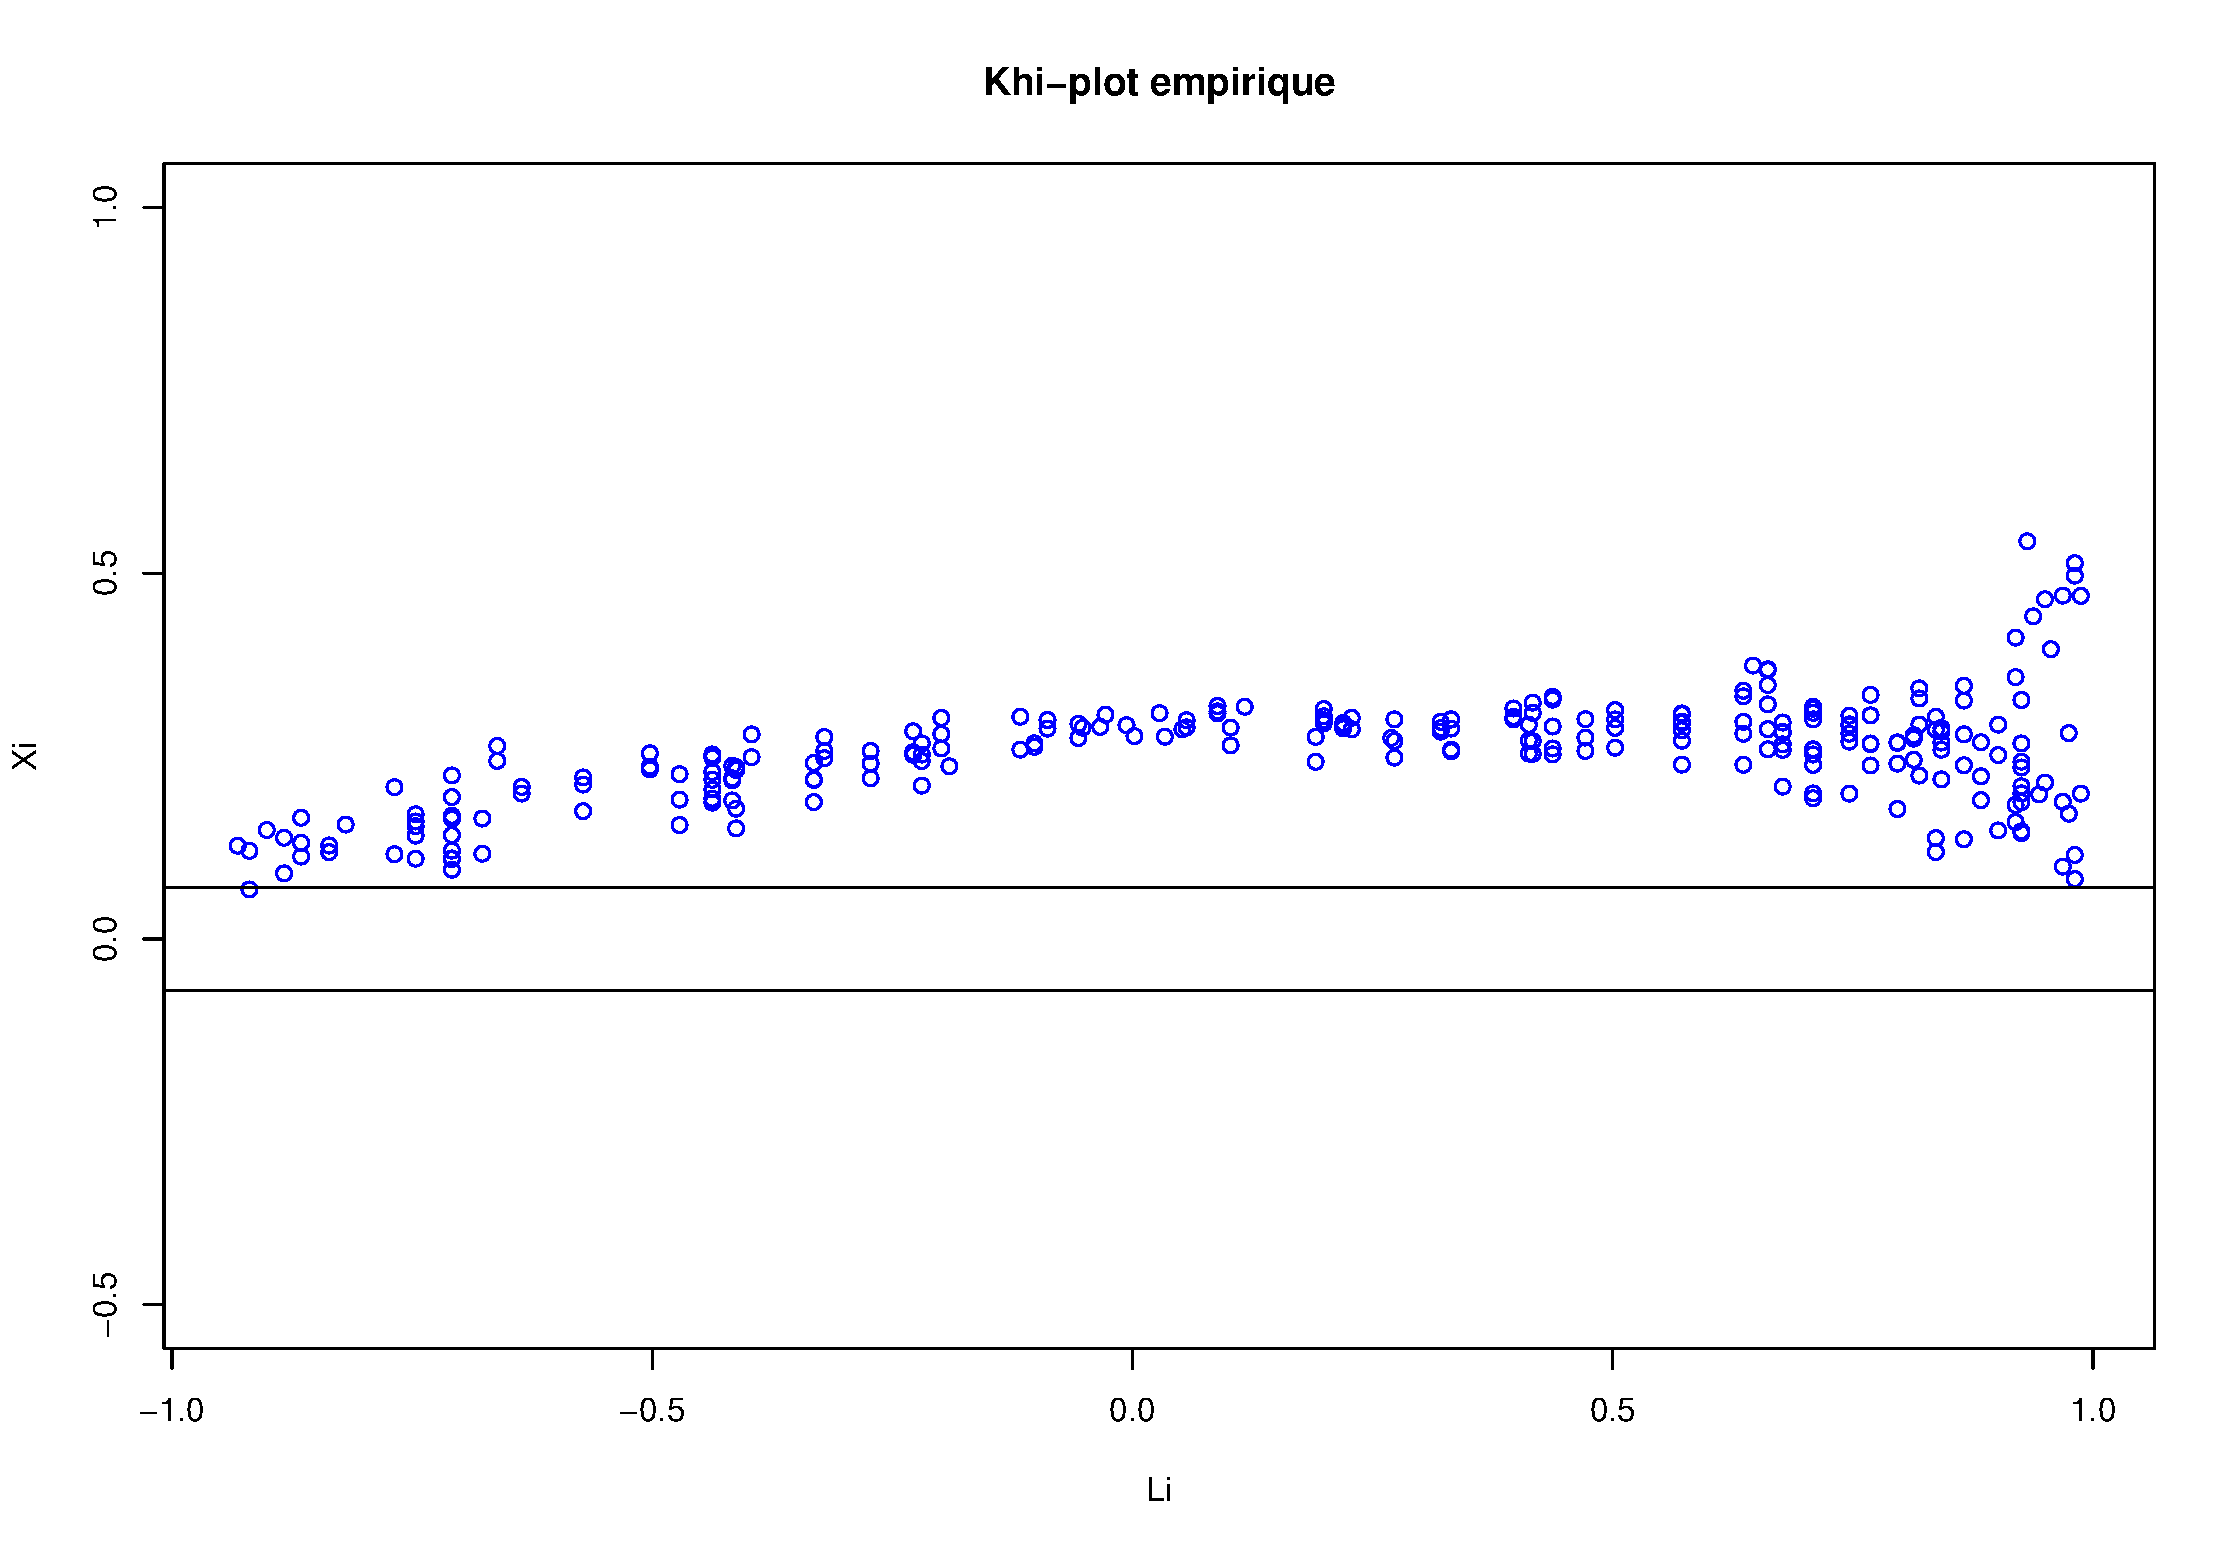
\includegraphics[width=14 cm, angle=0]{./pictures/chi_plot_empir.png}
      \centering\caption{Khi-plot empirique}
    \end{center}
\end{figure}



\subsection{K-plot ou diagramme de Kendall}

Le diagramme de Kendall est un aussi outil intéressant lorsque que l'on veut étudier la dépendance entre les variables d'intérêts.

Le K-plot introduit par Genest et Boies (2003) est l'équivalent pour les copules du Q-Q Plot pour les
densités univariées.

Pour détecter la dépendance entre deux variables $X$ et $Y$ dont les observations sont données par les vecteurs aléatoires $(X_1,...,X_n)$ et
$(Y_1,...,Y_n)$, on peut construire ce diagramme comme suit.

\begin{enumerate}
\item pour $i=1,...,n$, on calcule les pseudo-observations $H_i = \frac{1}{n-1} \# \{j \neq i : x_j \leq x_i, y_j \leq y_i \}$
\item on déduit les statistiques d'ordre associés : $H_{(1)} \leq ... \leq H_{(n)}$
\item on représente graphiquement les points $(W_{i:n},H_{(i)})$ où $W_{i:n}$ est l'espérance de la i-ème statistique d'odre 
d'un échantillon de taille $n$ de la distribution $K_0$ des $H_i$ sous l'hypothèse nulle d'indépendance.
\end{enumerate}

En utilisant des résultats classiques sur les statistiques d’ordre, on obtient que $W_{i:n}$ est égal à :

$$
W_{i:n}= n {n-1 \choose i-1} \int\limits_{0}^1 \omega k_0(\omega) ( K_0(\omega) )^{i-1} ( 1-K_0(\omega) )^{n-i} d\omega, 
$$

Avec :

\begin{itemize}
\item $K_0$ la loi asymptotique des $H_i$, $i=1...n$ sous l’hypothèse nulle d’indépendance définie par $K_0(\omega) = \omega - \omega \operatorname{log} (\omega), \omega \in (0,1)$;
\item $k_0$ est la densité des $H_i$, $i=1...n$ sous l’hypothèse d’indépendance, soit $K_0(\omega) = \int_0^\omega k_0(t)dt$.
\end{itemize}

Nous pouvons dès lors tracer le K-plot sur notre échantillon de données.

\noindent%
\begin{figure}[H]
    \begin{center}
      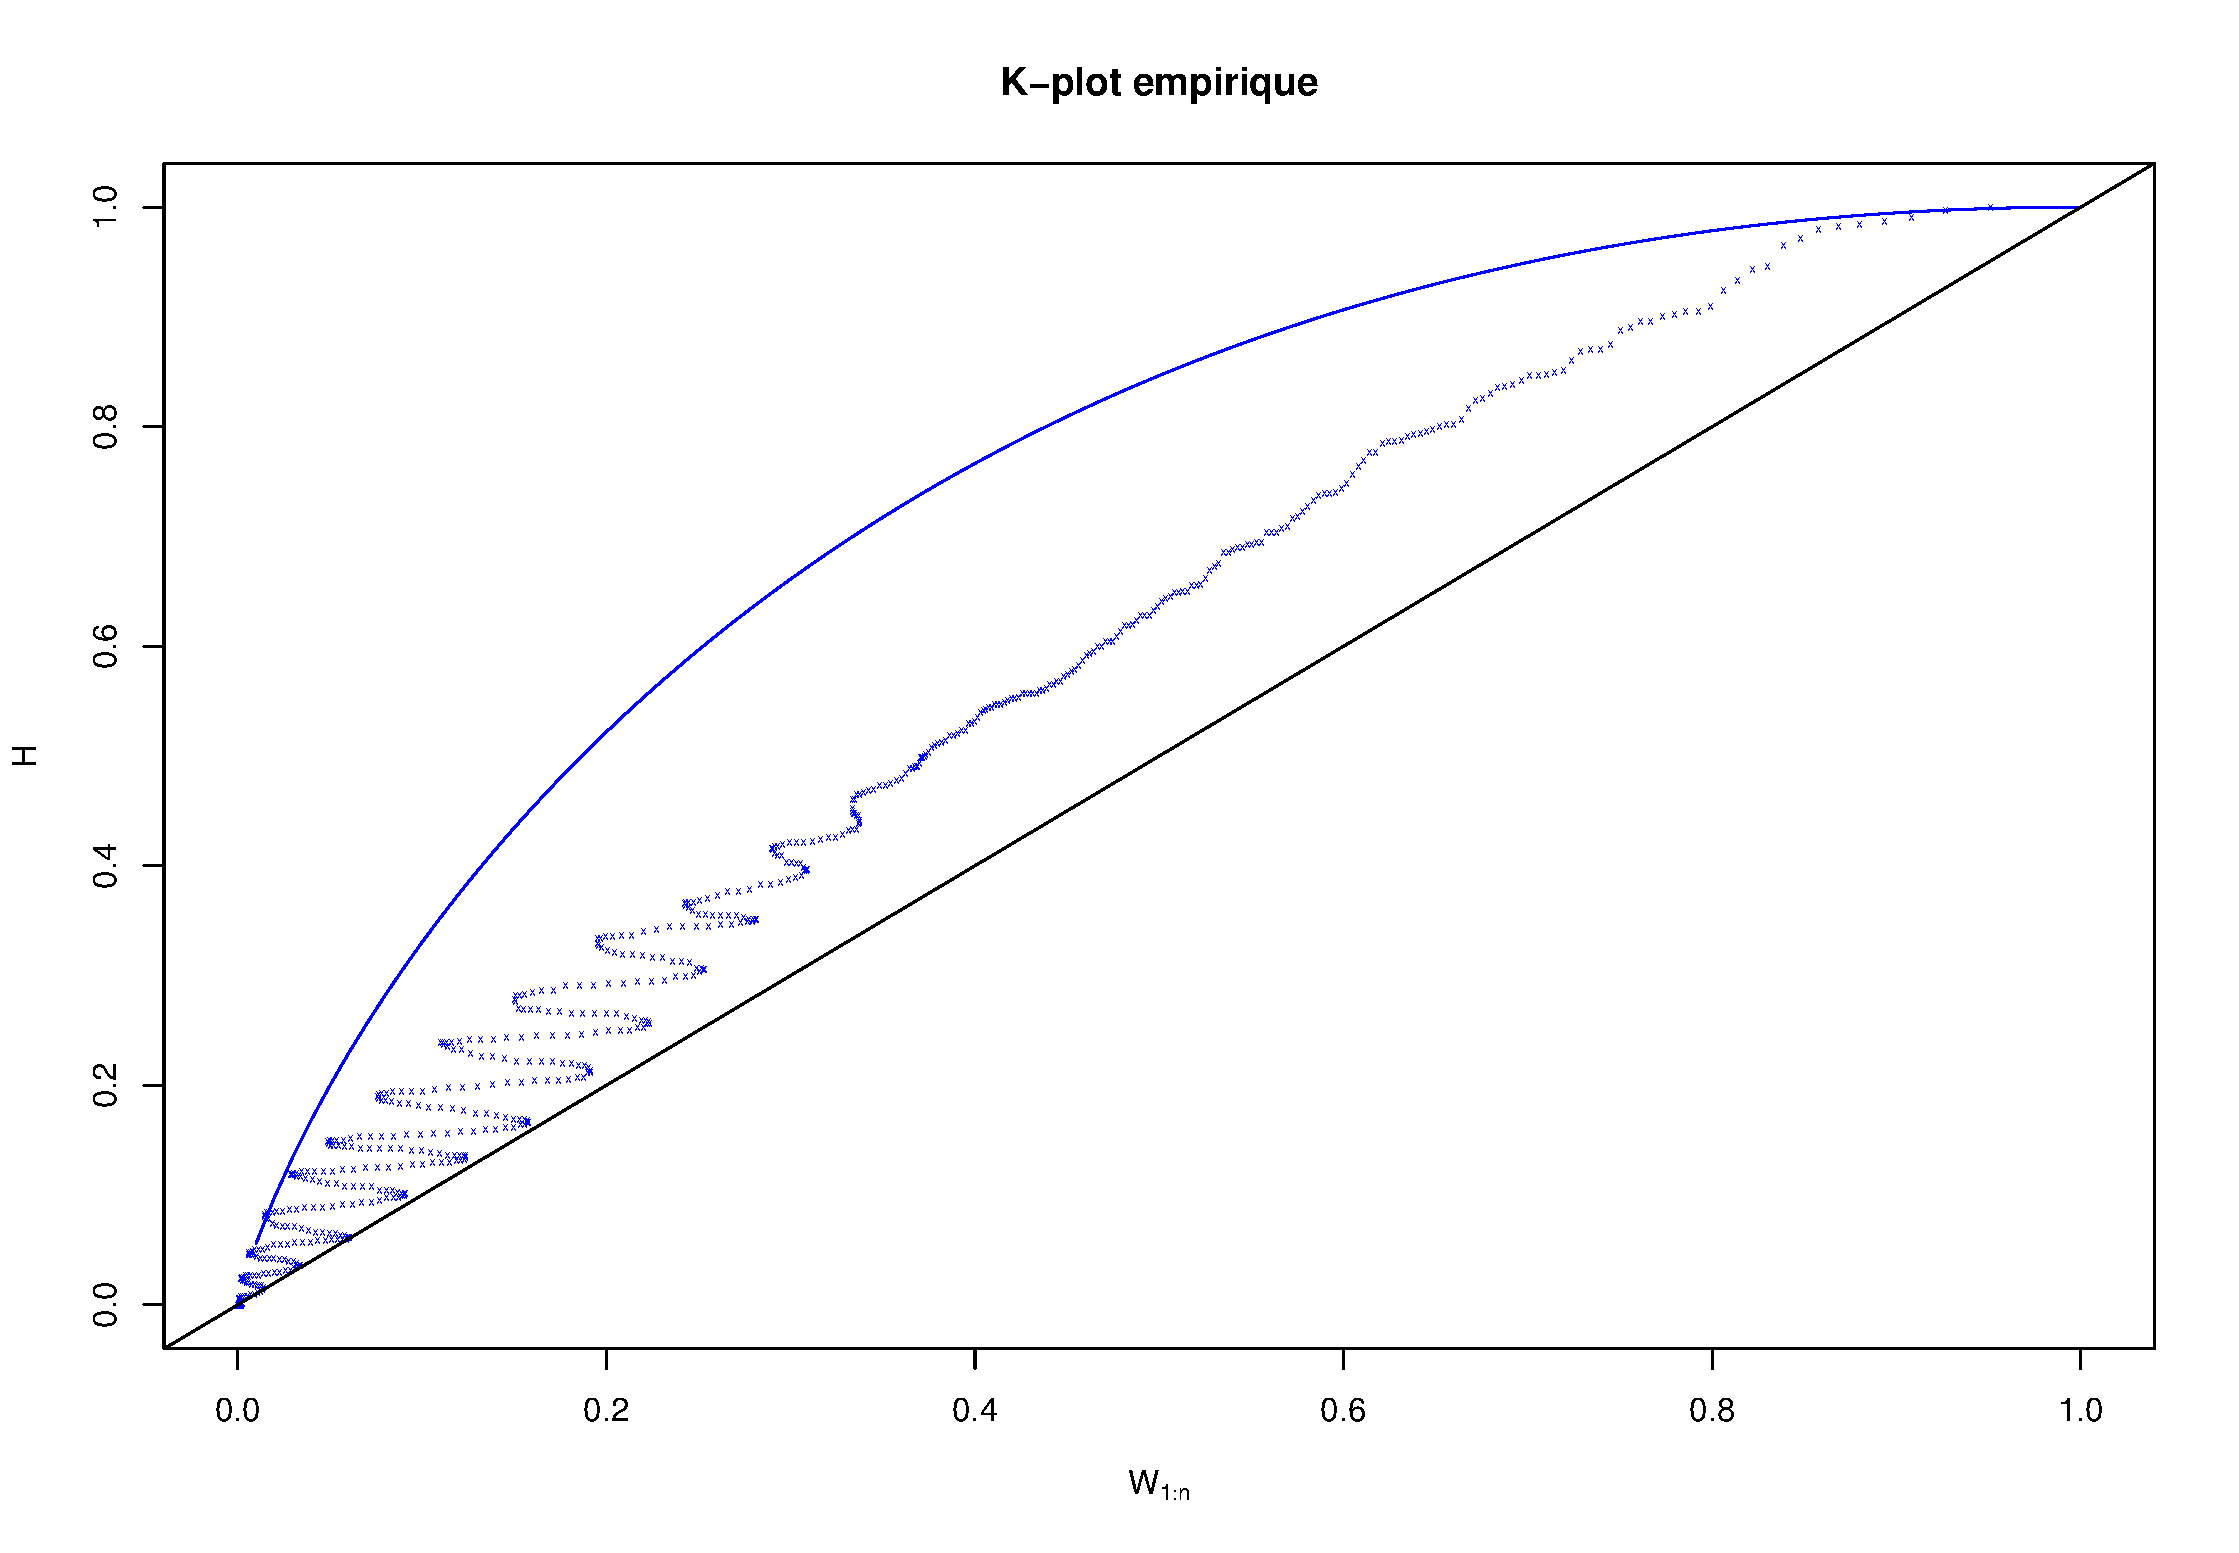
\includegraphics[width=14 cm, angle=0]{./pictures/K_plot_empir.png}
      \centering\caption{K-plot empirique}
    \end{center}
\end{figure}

Si $X$ et $Y$ étaitent indépendants, le Kendall-plot tendrait vers la linéarité.
Si $X$ et $Y$ étaient antimonotones, le Kendall-plot serait aligné sur l'axe horizontal.
En revanche, si $X$ et $Y$ étaient comonotones, le Kendall-plot serait aligné sur la courbe d’équation $\omega \longrightarrow K_0(\omega) = \omega - \omega \operatorname{log} (\omega)$.

Ainsi, nous pouvons observer que les variables aléatoires $X$ et $Y$ montrent une nouvelle fois la dépendance positive qui les lie.

\section{Méthode non paramétrique d'estimation : la copule empirique}
%%%%%%%%%%%%%%%%%%%%%%%%%%%%%%%%%%%%%%%%%%%%%%%%%%%%%%%%%%%%%%%%%%%%%%%

\subsection{Copule empirique de Deheuvels}

La copule empirique a été introduite par Paul Deheuvels (1979). 

Cette méthode repose sur le rang des observations pour extraire ensuite la
structure de dépendance.

On se place dans notre cas où l'on a un échantillon bivarié.

Soit $(x_i,y_i)_{1 \leq i \leq n}$ un échantillon d'observation de taille $n$ de $(X,Y)$ 
et soit $(r_i,s_i)_{1 \leq i \leq n}$ la statistique de rang associé à cet échantillon bivarié.

La copule empirique de Deheuvels, dans le cas bivarié, est définie sur l'ensemble $\left \{ \left( \frac{i}{n} , \frac{j}{n} \right) , 0 \leq i,j \leq n   \right \}$ 
par l'équation suivante :
\begin{eqnarray*}
C_n \left( \frac{i}{n},\frac{j}{n}\right) &=& \frac{1}{n} \sum_{k=1}^n \mathbb{1}_{r_k \leq i} \mathbb{1}_{s_k \leq j} \\
 &=& \frac{1}{n} \sum_{k=1}^n \mathbb{1}_{ \{r_k \leq i\} \cap \{ s_k \leq j\} } 
\end{eqnarray*}

Finalement, similairement au calcul de la fonction de répartition empirique, la formule ci-dessus sur l'ensemble $\left \{ \left( \frac{i}{n} , \frac{j}{n} \right) , 0 \leq i,j \leq n   \right \}$ revient à écrire :

$\forall (u,v) \in [0,1]^2$,
$$
C_n(u,v) = \frac{1}{n} \sum_{k=1}^n \mathbb{1}_{ \{ \frac{r_k}{n} \leq u\} \cap \{ \frac{s_k}{n} \leq v\} } 
$$

La copule empirique n’est autre que la fonction de répartition bivariée associée au nuage de point $\left( \frac{r_i}{n},\frac{s_i}{n} \right )_{1 \leq i \leq n}$.

Cet estimateur possède l'avantage de ne pas dépendre des distributions marginales. De plus, la copule
empirique d'ordre n $C_n$ converge asymptotiquement vers la copule $C$ d'après Faivre (2002).

Une fois la copule empirique calculée, nous pouvons tout d'abord tracer un graphique 3D afin d'avoir une
idée de la forme de notre copule :

\noindent%
\begin{figure}[H]
    \begin{center}
      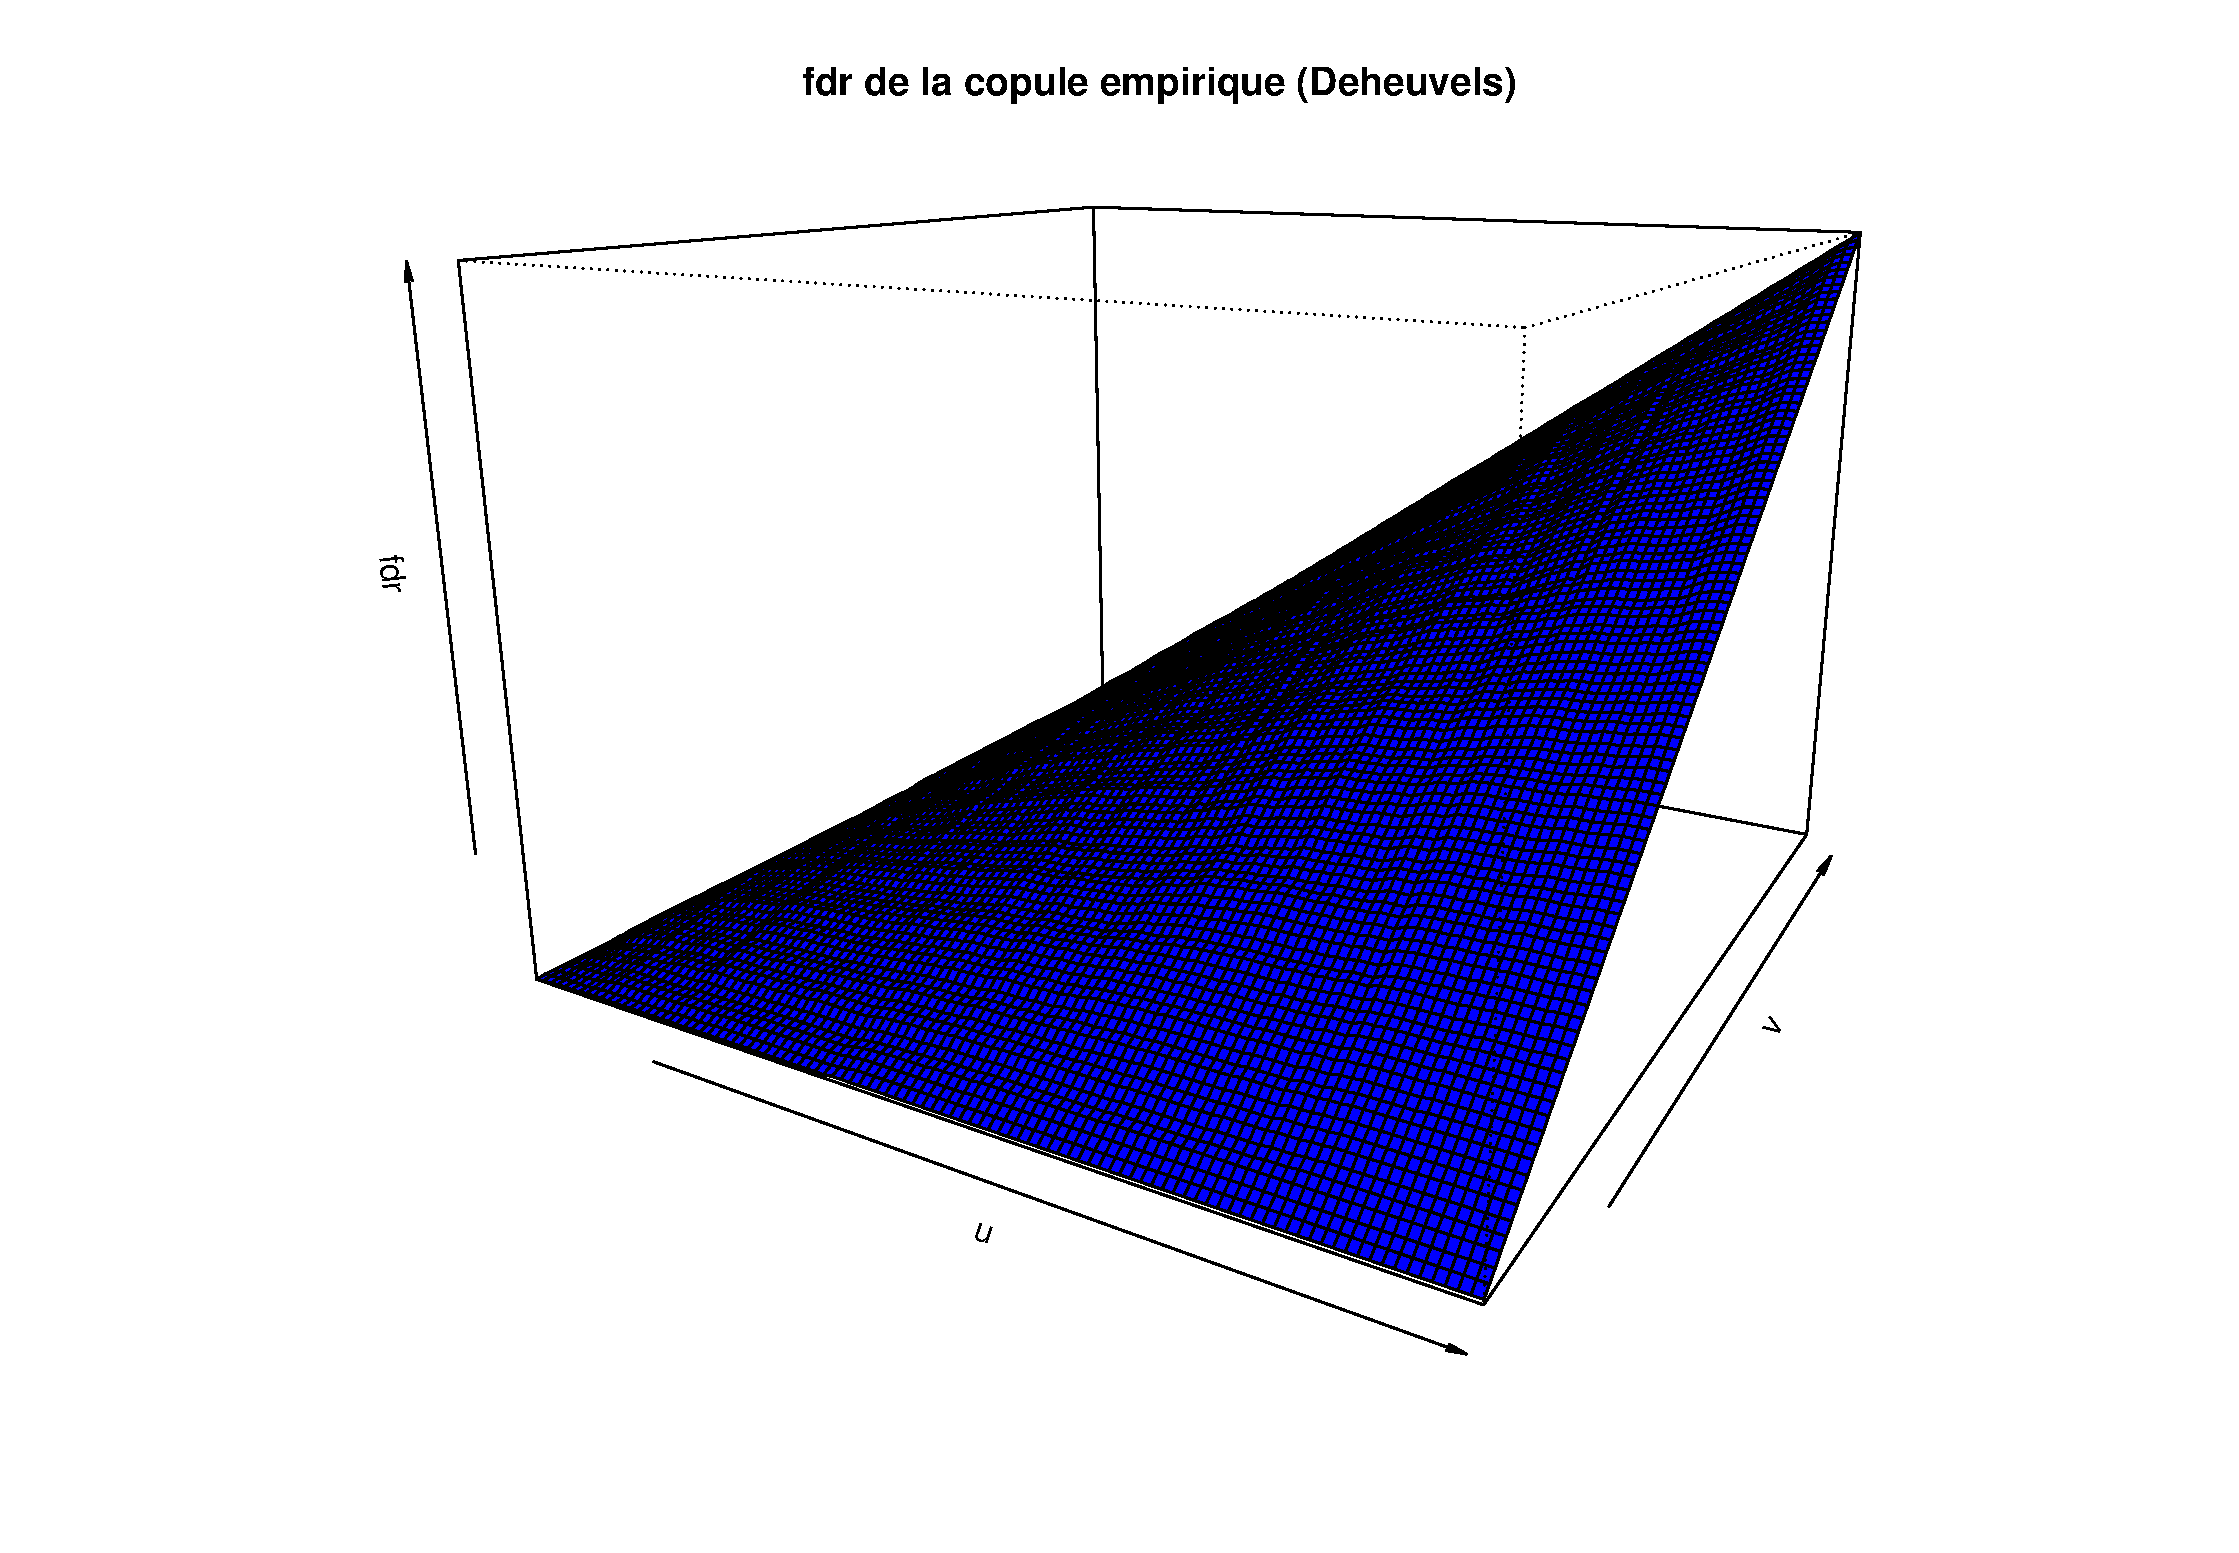
\includegraphics[width=14 cm, angle=0]{./pictures/copule_empirique.png}
      \centering\caption{\label{graph_cop_empir}Fonction de répartition de la copule empirique}
    \end{center}
\end{figure}


Le graphique 3D d'une copule empirique tel que tracé sur la figure \ref{graph_cop_empir} est difficilement exploitable.
Nous allons donc devoir construire d'autres indicateurs plus visuels d'où il sera possible de tirer des
informations utiles à la sélection de notre copule théorique.



\subsection{Dépendance de queue}

Disposant à présent d'un estimateur de la copule, nous pouvons aisément étudier les dépendances de queue à l'aide des estimateurs de Caillault et Guégan 
présentés dans la section précédente.

Nous obtenons les graphiques suivants :

\noindent%
\begin{figure}[H]
    \begin{center}
      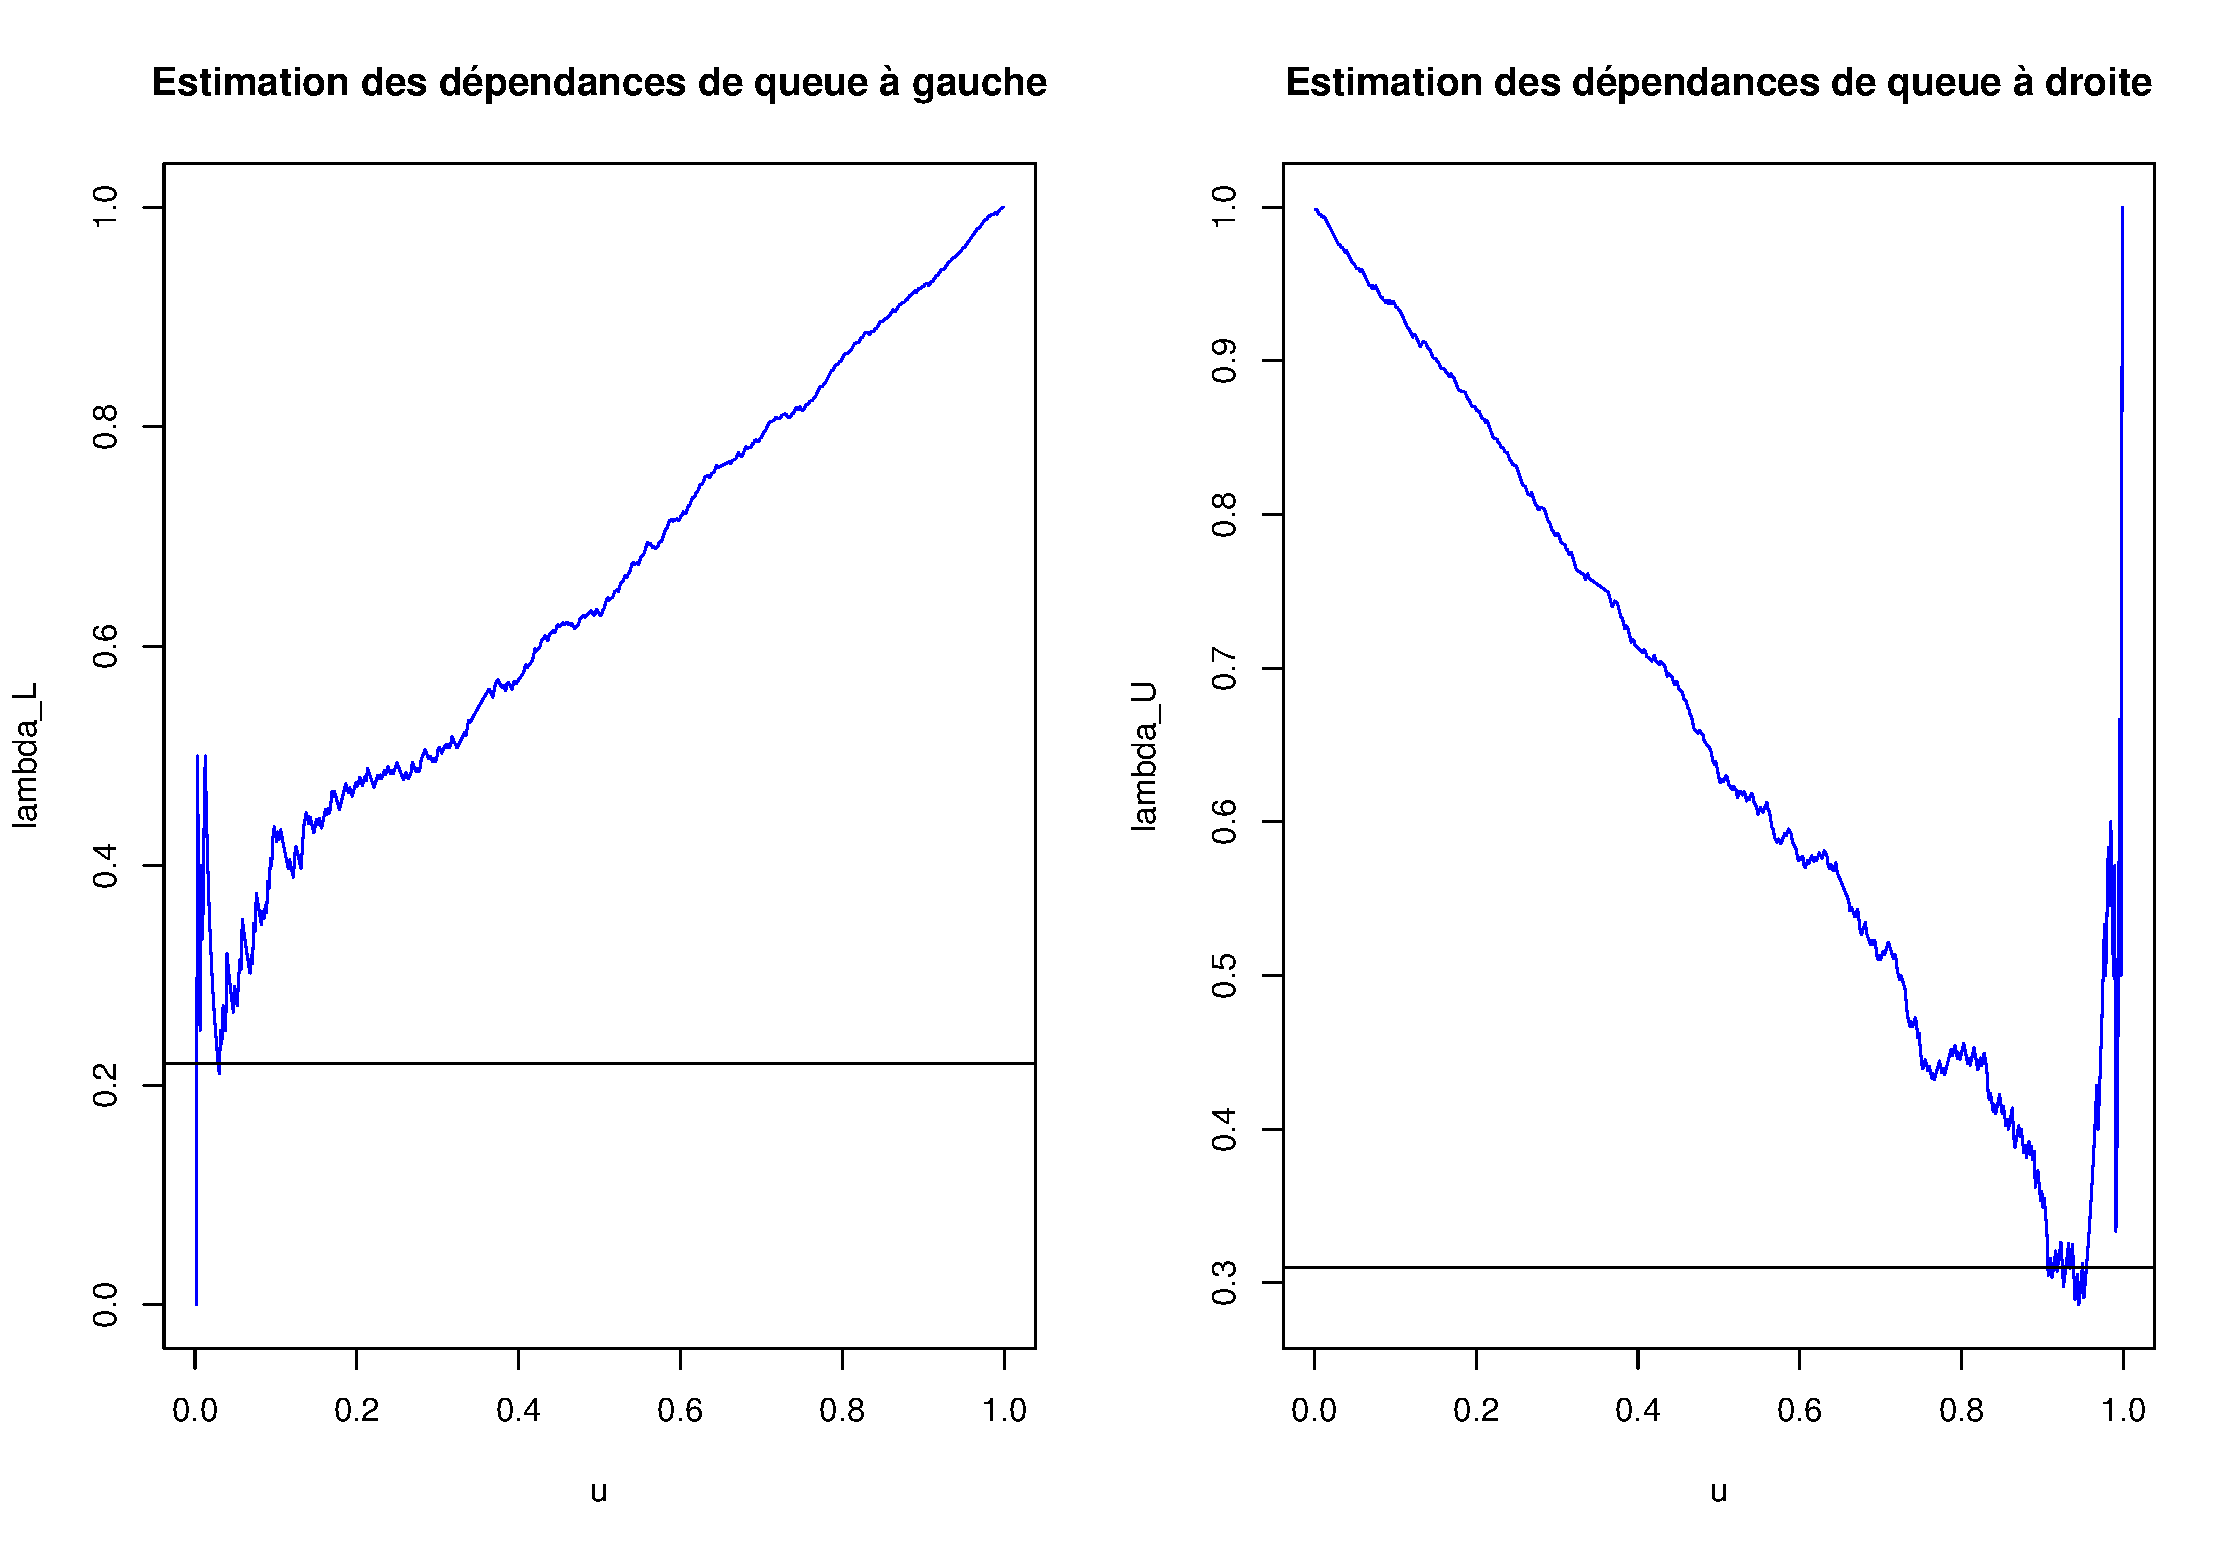
\includegraphics[width=14 cm, angle=0]{./pictures/dependance_queue_empir.png}
      \centering\caption{Estimation des dépendances de queue à gauche et à droite}
    \end{center}
\end{figure}

D'après les définitions vues plus haut pour les quantités $\lambda_L$ et $\lambda_U$, on dit que la copule a une dépendance de queue à gauche
et à droite si respectivement les asymptotes en 0+ de $\lambda_L$ et en 1- de $\lambda_U$ sont différentes de 0.

Nous obtenons (grossièrement) une asymptote d'équation $y=0,22$ pour $\lambda_L$ et une asymptote d'équation $y=0,31$ pour $\lambda_U$.

Nous remarquons que les valeurs obtenues sont faibles mais ne peuvent pas être considérées comme nulles. Les dépendances de queue à gauche 
et à droite existent bien.


\subsection{Histogramme 3D}

Pour poursuivre notre étude, nous pouvons représenter un histogramme en trois dimensions, utilisant les rangs des données comme pour le rank-rank plot, sur une grille $10 \times 10$.

\noindent%
\begin{figure}[H]
    \begin{center}
      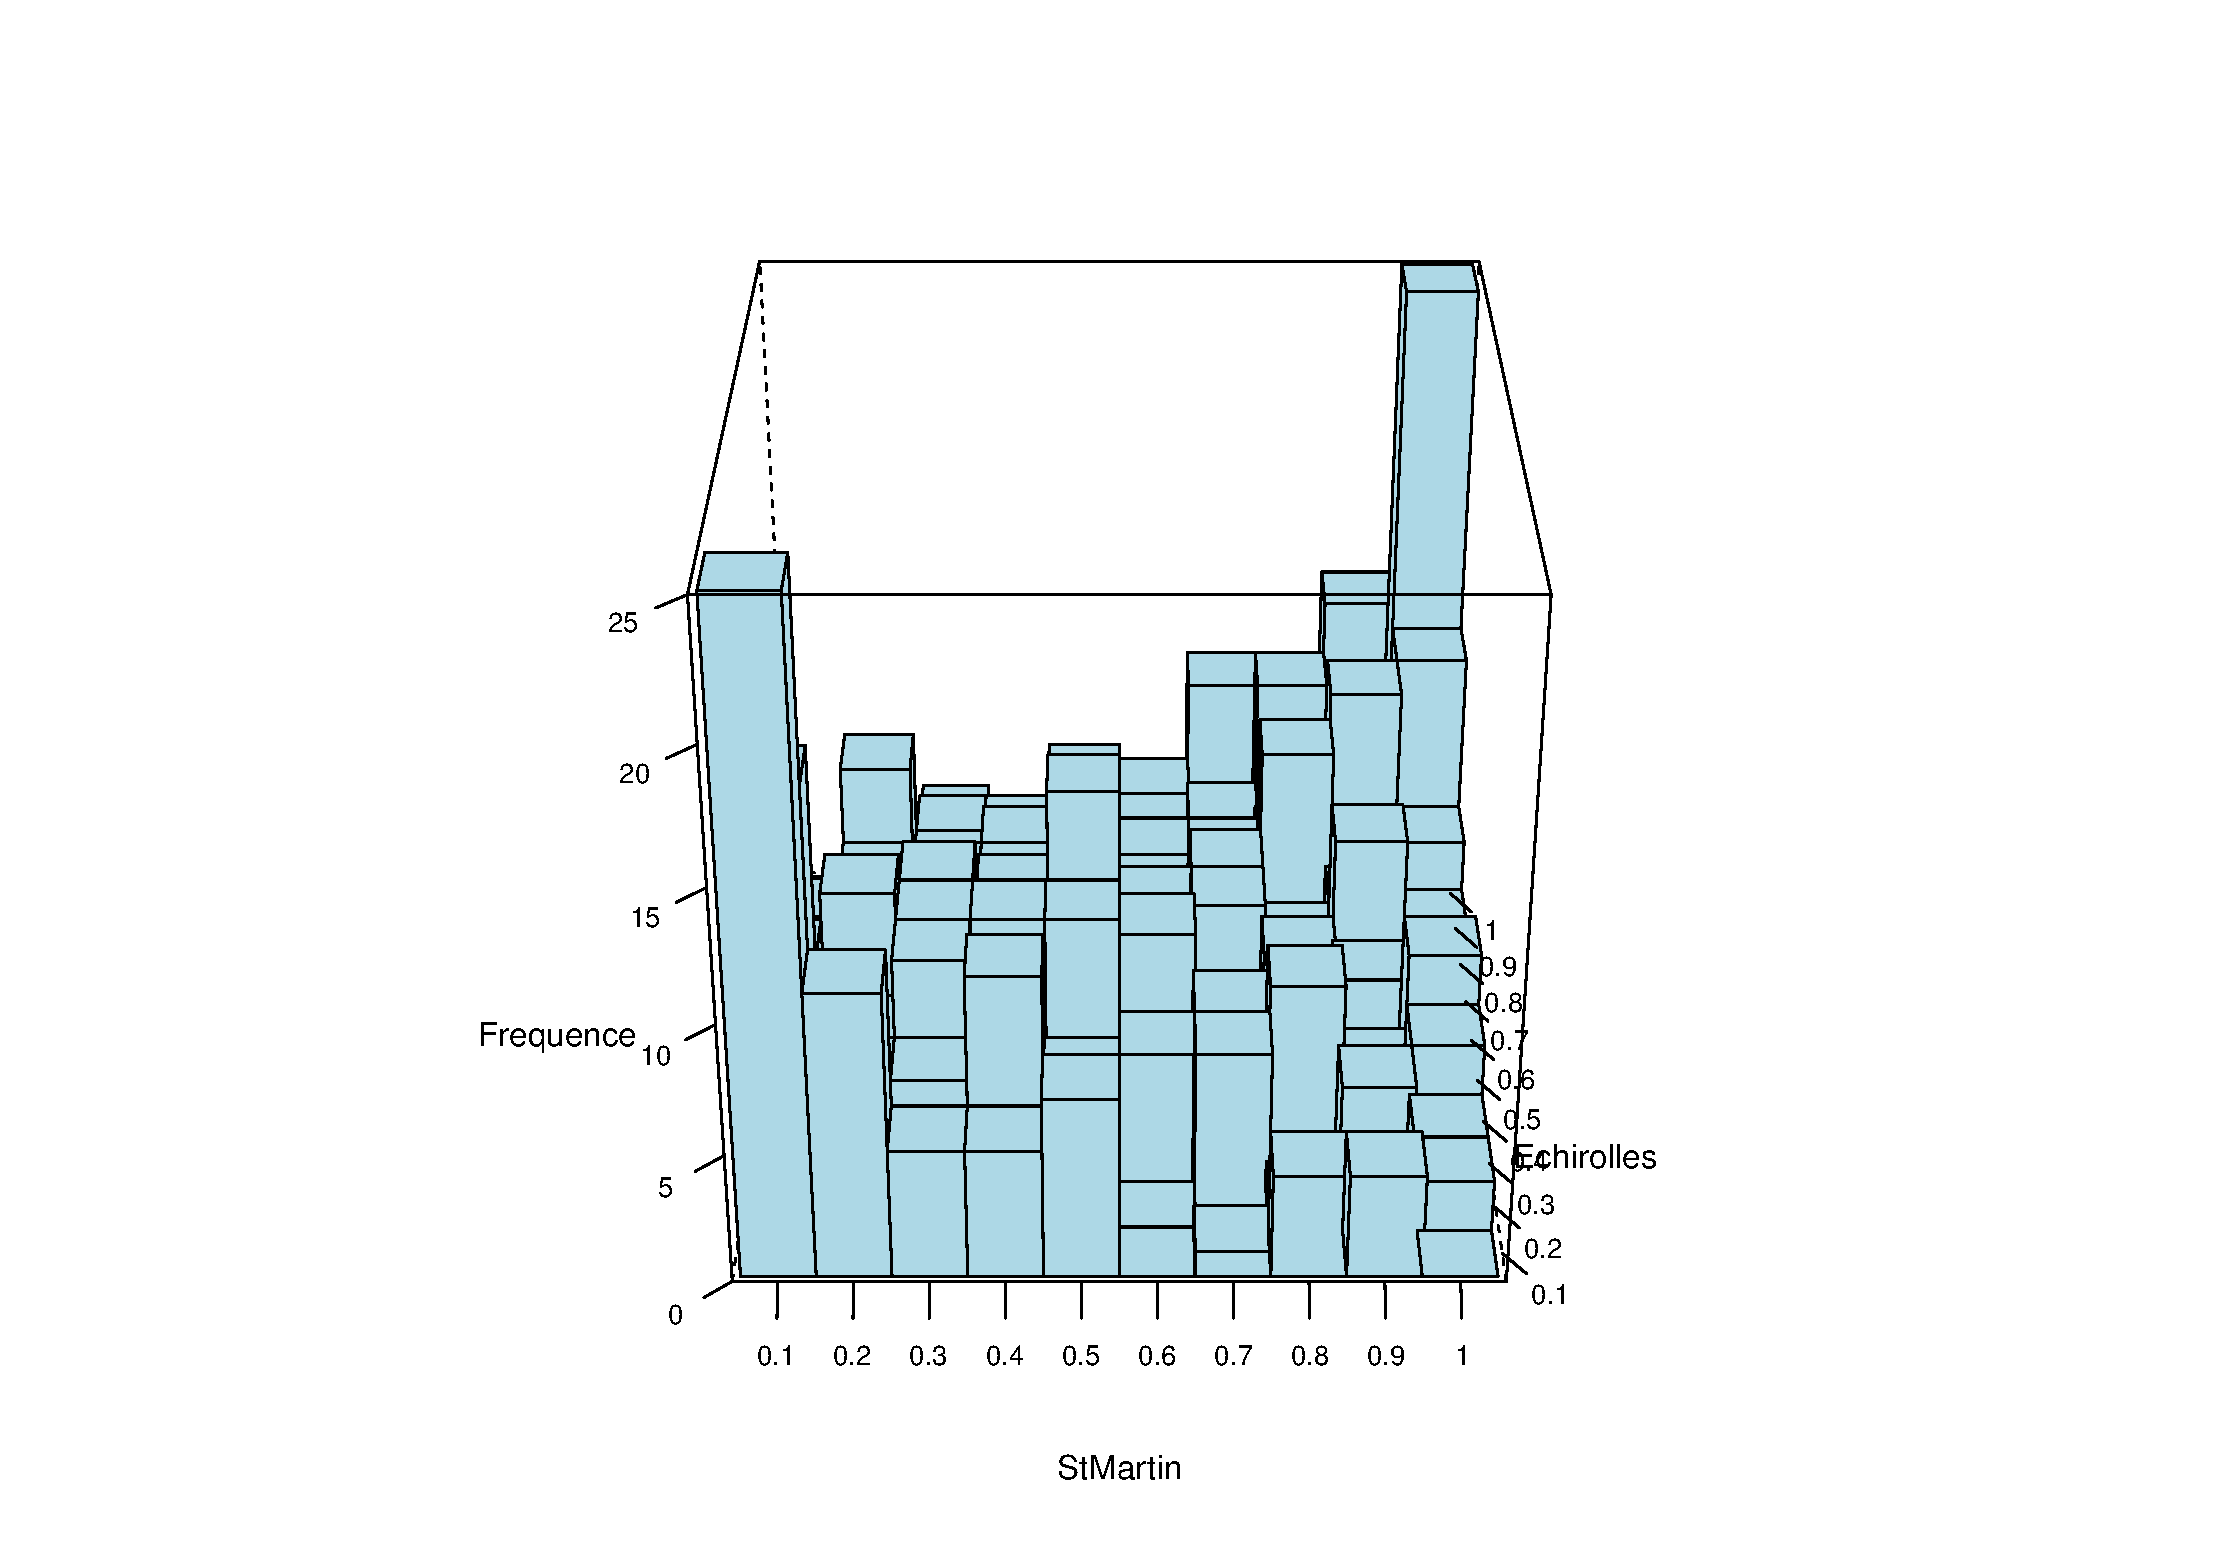
\includegraphics[width=14 cm, angle=0]{./pictures/hist3d.png}
      \centering\caption{Histogramme 3D sur une grille 10 X 10 des rangs des données}
    \end{center}
\end{figure}

On peut ainsi remarquer une fois de plus la dépendance positive de la copule, mais également les dépendances de queue à gauche et droite, qui semblent apparaître nettement sur ce graphe.

\subsection{Fonction de densité empirique}

La fonction de distribution empirique de la copule proposée par Deheuvels présente certains inconvénients.
En effet, Deheuvels donne un estimateur de la copule empirique sur l'échantillon considéré en utilisant la 
fonction de répartition.

Comme nous l'avons déjà mentionnée plus haut, elle a pour expression :

\begin{eqnarray*}
C_n \left( \frac{i}{n},\frac{j}{n}\right) = \frac{1}{n} \sum_{k=1}^n \mathbb{1}_{ \{r_k \leq i\} \cap \{ s_k \leq j\} } 
\end{eqnarray*}
sur l'ensemble $\left \{ \left( \frac{i}{n} , \frac{j}{n} \right) , 0 \leq i,j \leq n   \right \}$.

Cette fonction cumulative est fortement discontinue, faisant apparaître une caractéristique par paliers avec des probabilitées cumulées constantes
entre chaque point et des sauts à chaque observation.

Cela n'est pas très gênant pour une fonction de distribution mais le devient si on déduit la fonction de densité. La fonction de densité de la structure de dépendance 
empirique peut être directement déduite de sa fonction de distribution :

$$
c_n \left( \frac{i}{n},\frac{j}{n}\right) = \sum_{k=1}^2 \sum_{l=1}^2 (-1)^{(k+l)} C_n \left( \frac{i-k+1}{n},\frac{j-l+1}{n}\right)
$$

Le but ici est de proposer un nouvel estimateur de la fonction de densité de la structure de dépendance empirique en inversant la méthode du noyau.
D'après Silverman (1986), l'estimation non paramétrique par la méthode des noyaux peut s'appliquer à des données multivariées, et en l'occurence bivariées.

En univarié, l'estimateur de la densité s'écrit :

$$
\widehat{f}(x) = \frac{1}{nh} \sum_{i=1}^n K \left( \frac{x - x_i}{h} \right)
$$
où $K$ est la fonction noyau vérifiant $\int_\mathbb{-\infty}^{+\infty} K(x)dx =1$.

Par exemple, le noyau gaussien se définit par :
$$
K(u) = \frac{1}{\sqrt{2 \pi}} e^{-\frac{u^2}{2}}
$$

En dimension 2, l'estimateur de la densité bivariée s'écrit :

$$
\widehat{f}(x,y) = \frac{1}{nh^2} \sum_{i=1}^n K \left(  \frac{x - x_i}{h} , \frac{y-y_i}{h}    \right)
$$
avec la condition que $$ \int_\mathbb{-\infty}^{+\infty}  \int_\mathbb{-\infty}^{+\infty} K(x,y) dx dy = 1$$

En somme, un estimateur à noyau de la densité de copule basé sur l’échantillon $\left(F_n(x_1),G_n(y_1)\right),...,\left(F_n(x_n),G_n(y_n)\right)$ est
donné par :

$$
c_n(u,v) = \frac{1}{nh^2} \sum_{i=1}^n K \left(  \frac{u - F_n(x_i)}{h} , \frac{v-G_n(y_i)}{h}    \right)
$$


Avec un noyau gaussien, nous obtenons le graphique suivant pour la fonction de densité empirique :

\noindent%
\begin{figure}[H]
    \begin{center}
      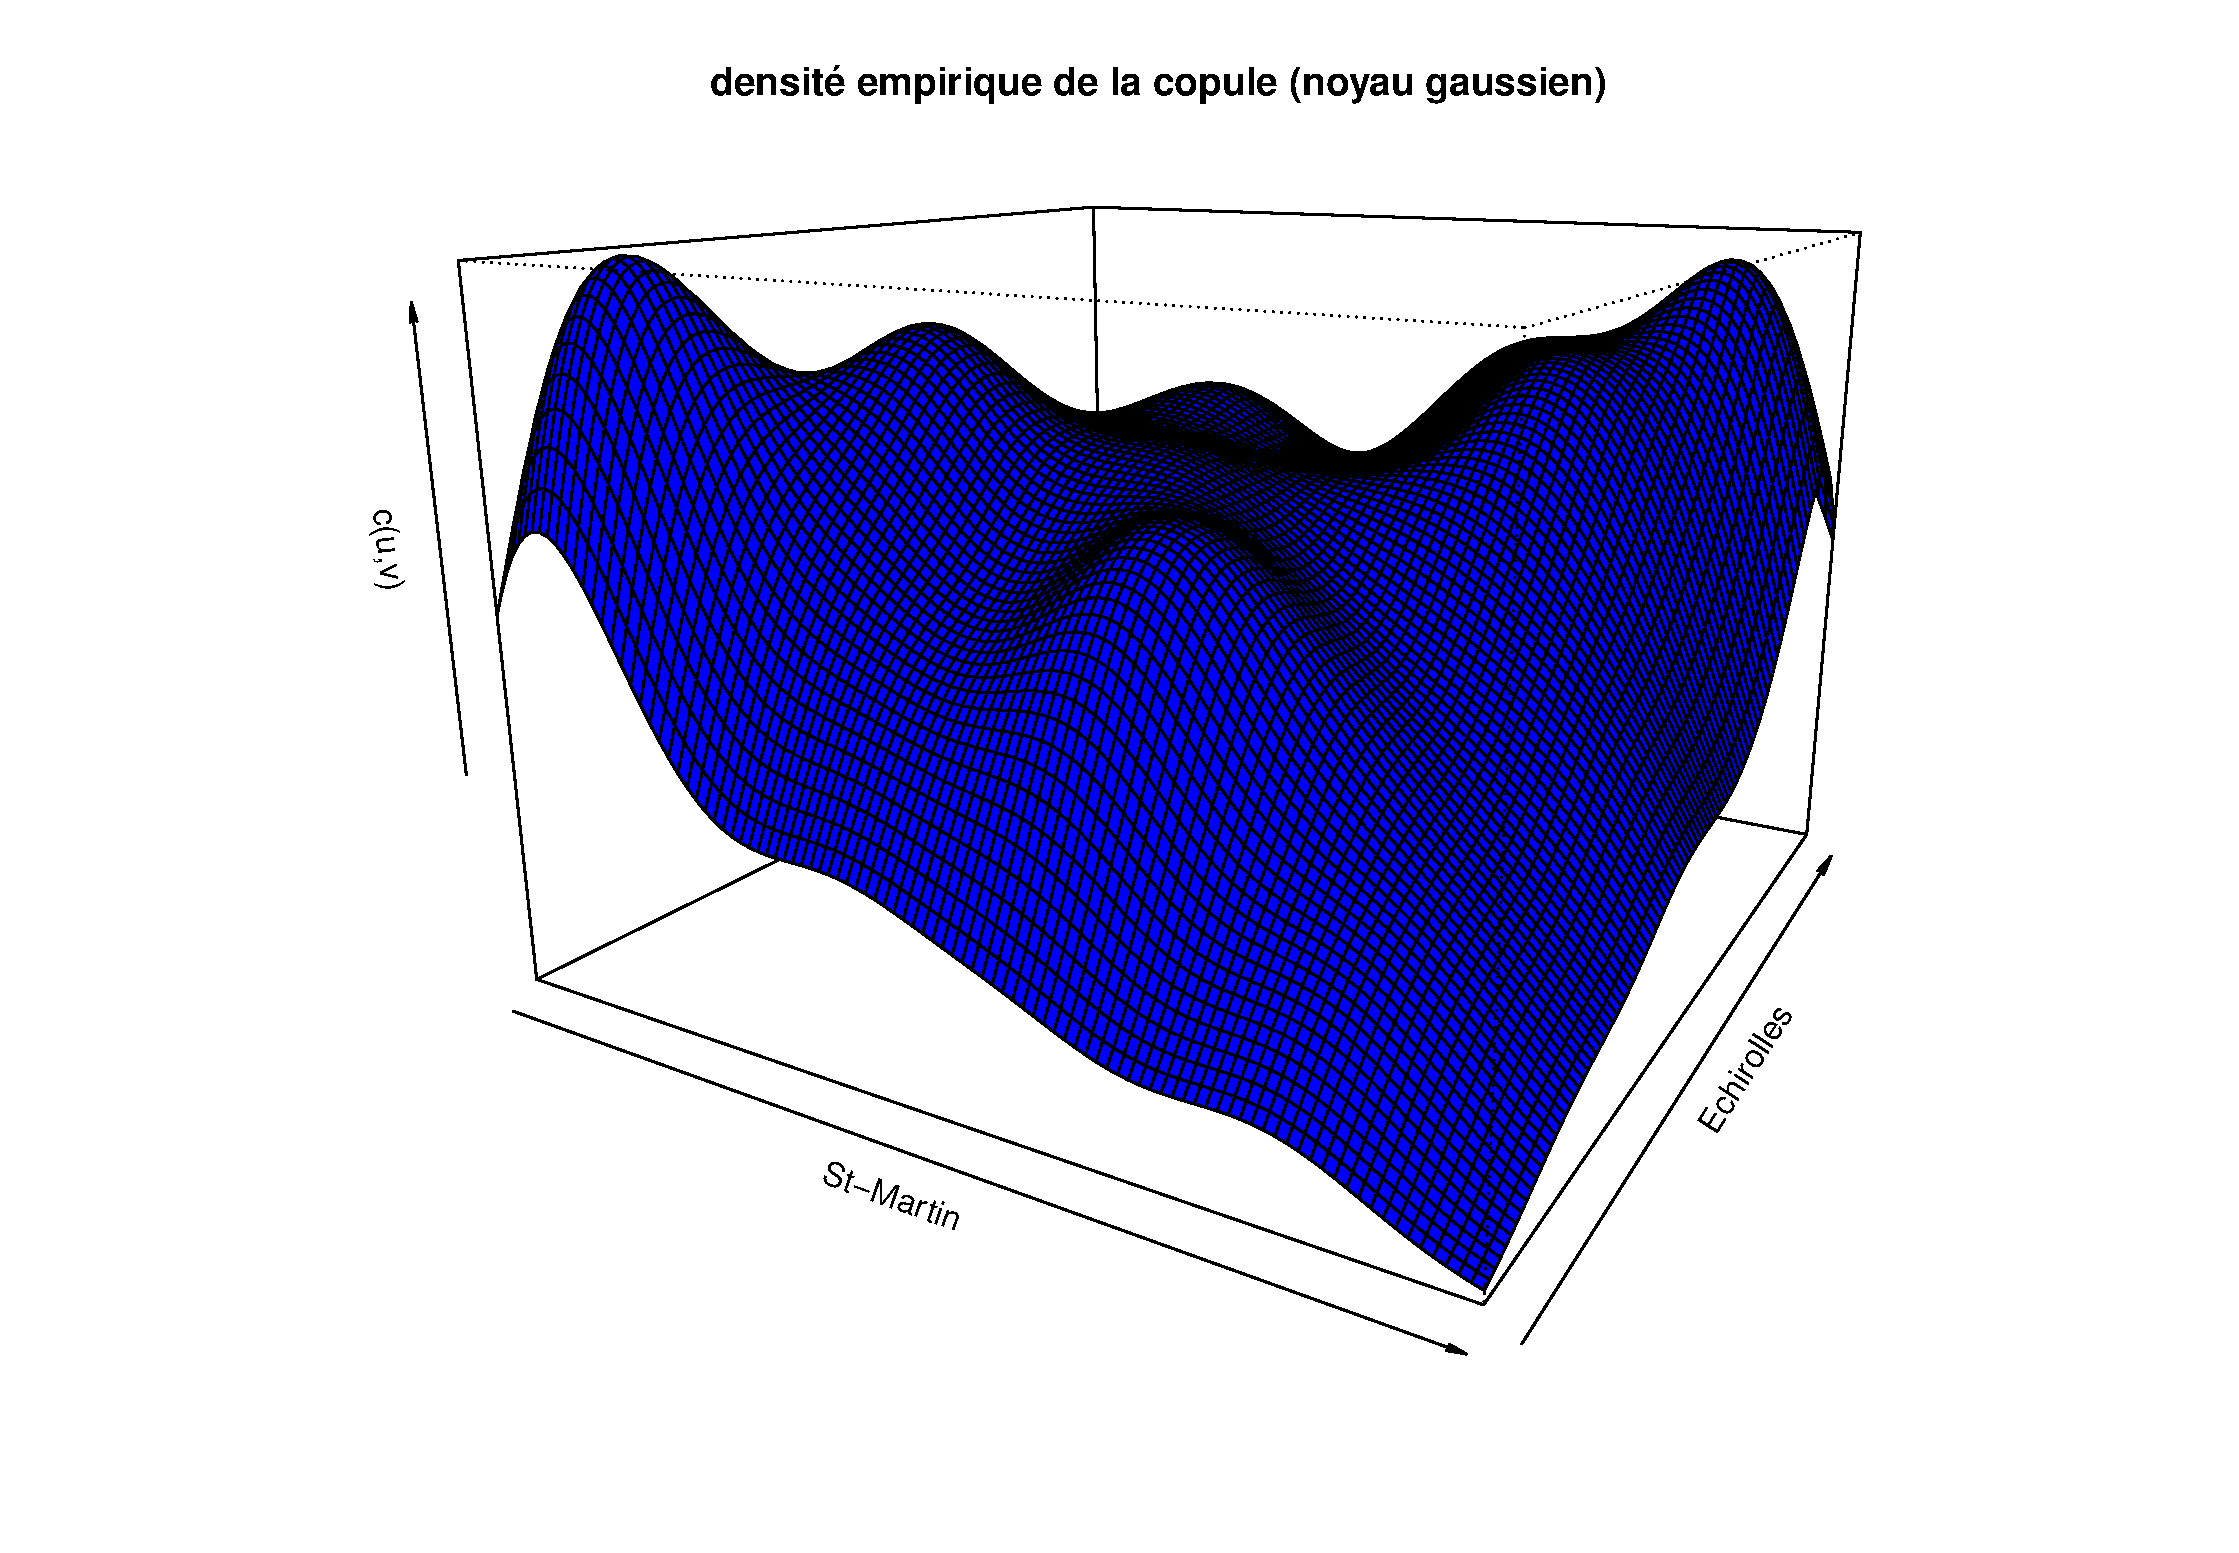
\includegraphics[width=16 cm, angle=0]{./pictures/densite_empir_gaussien.png}
      \centering\caption{Estimation de la fonction densité par noyau gaussien}
    \end{center}
\end{figure}

Avec le noyau d’Epanechnikov, nous obtenons l'estimation de la densité suivante :

\noindent%
\begin{figure}[H]
    \begin{center}
      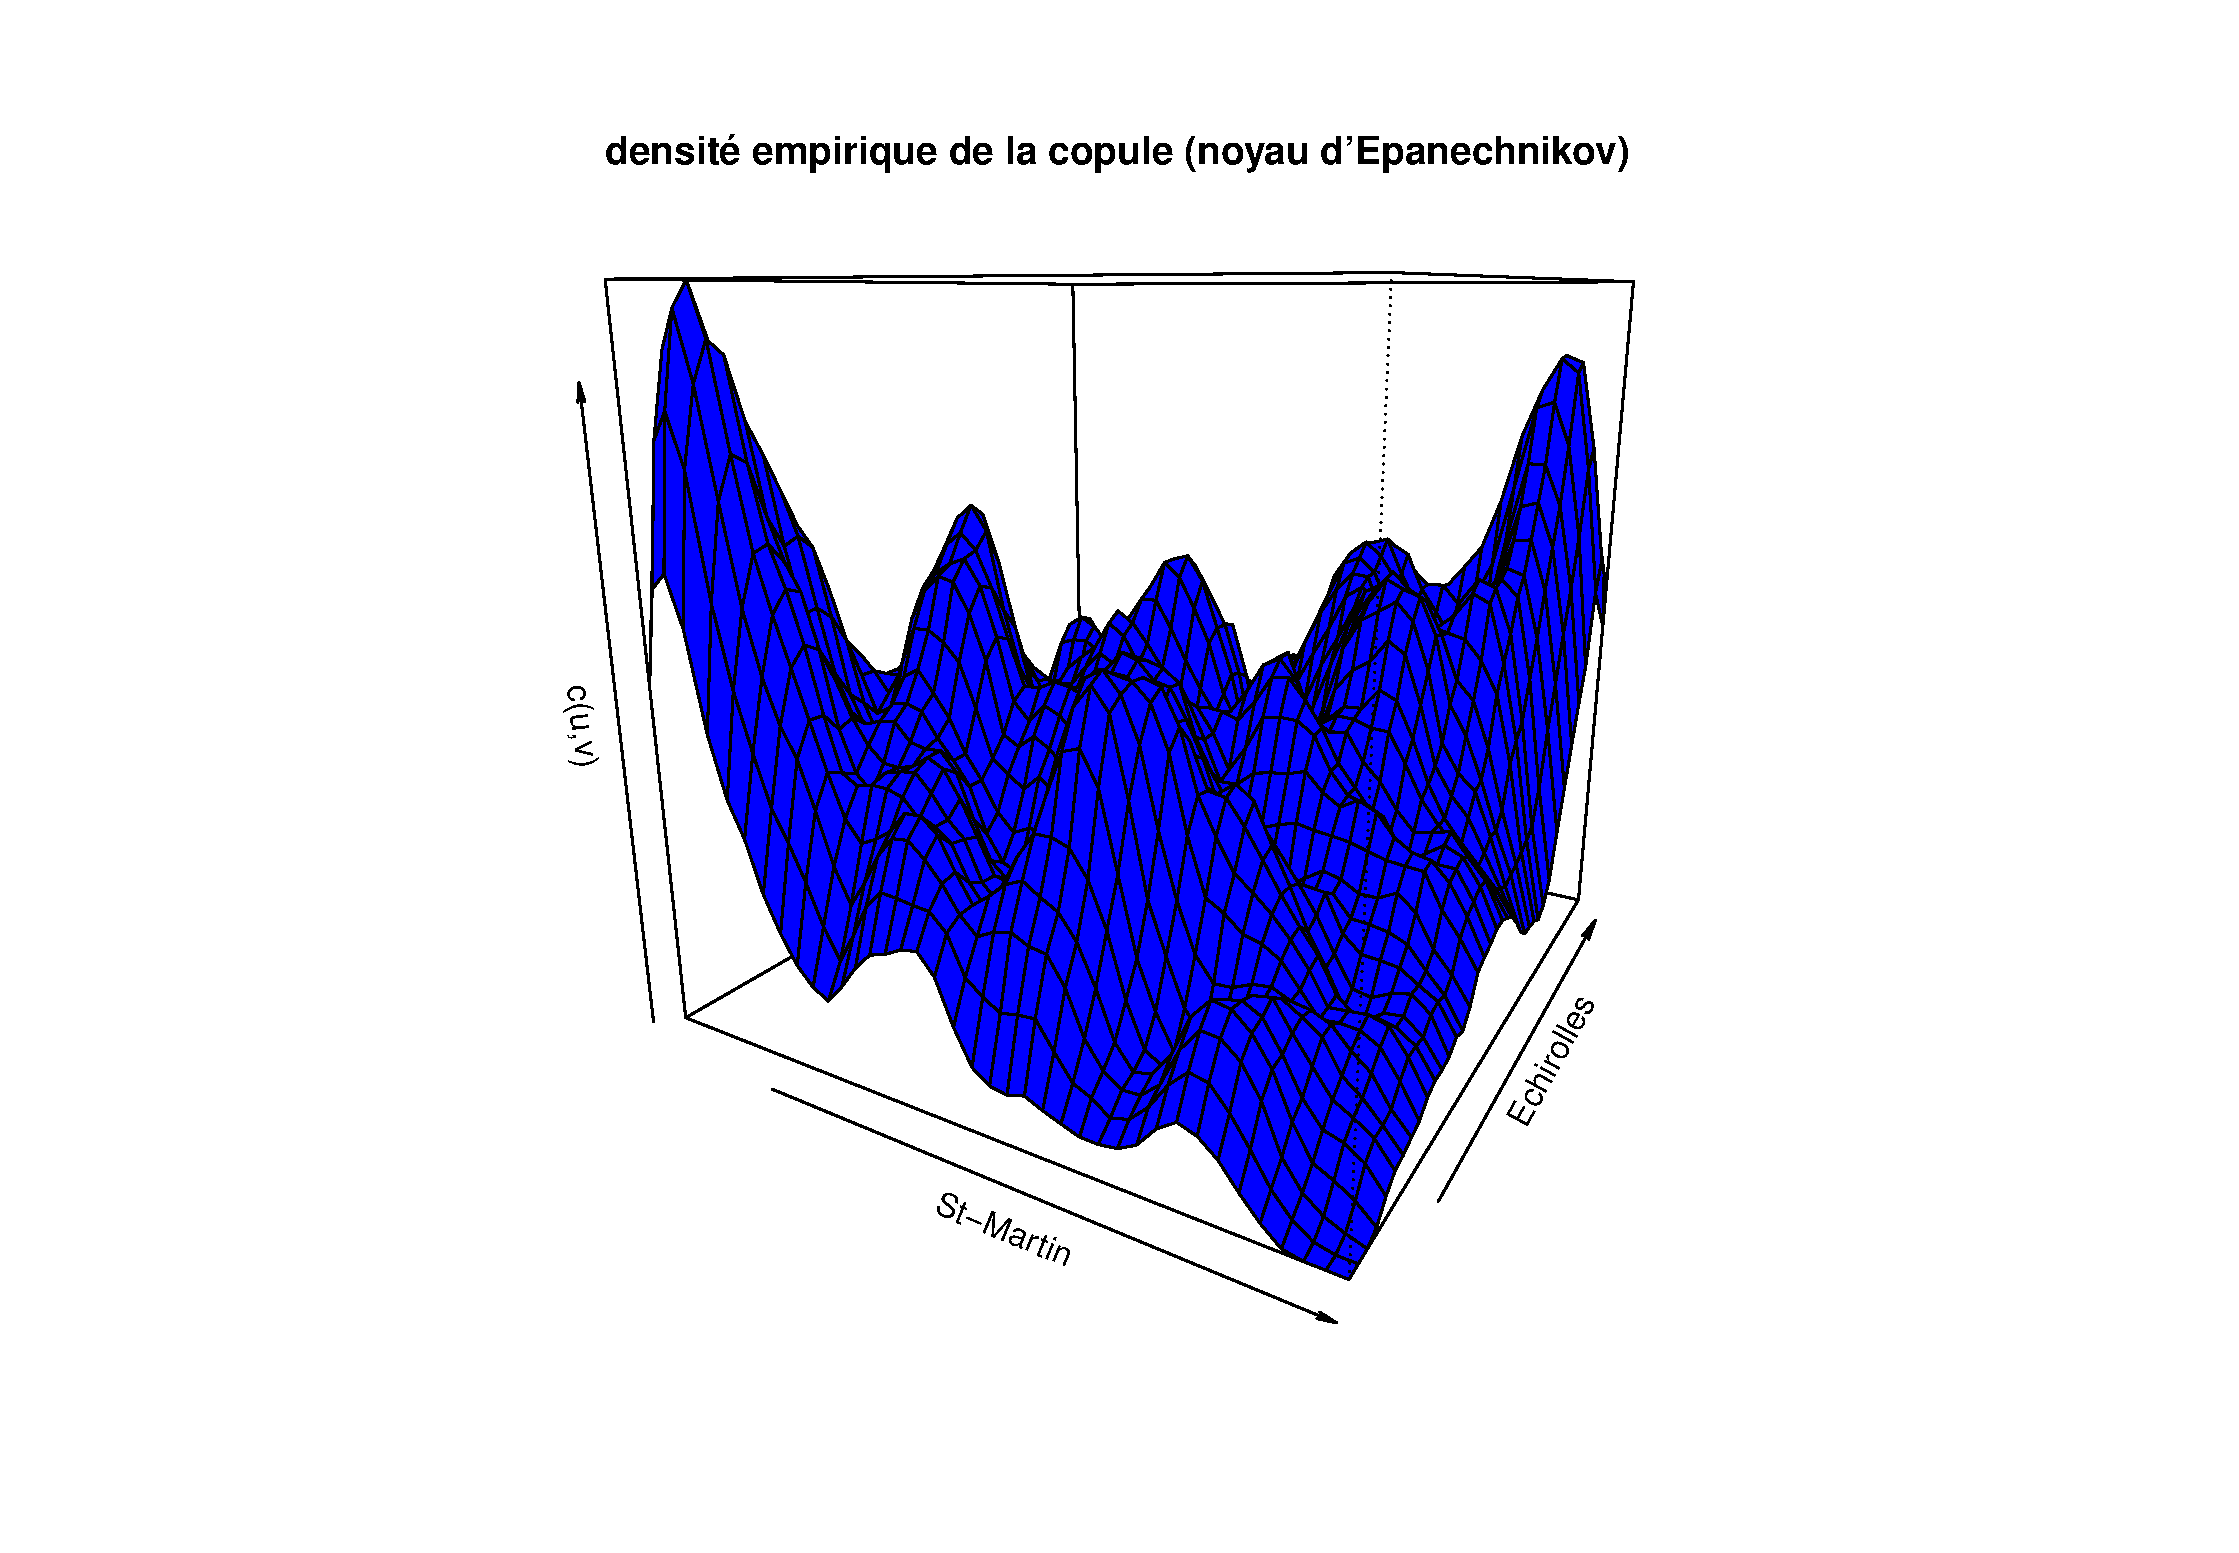
\includegraphics[width=16 cm, angle=0]{./pictures/densite_empir_Epanechnikov.png}
      \centering\caption{Estimation de la fonction densité par noyau d'Epanechnikov}
    \end{center}
\end{figure}

En observant ces graphiques, et afin de ne pas écarter d'emblée un modèle de copule, nous étudierons les copules candidates suivantes :
\begin{itemize}
\item Gumbel,
\item Clayton,
\item Frank 
\end{itemize}
qui sont des copules archimédiennes 

et les copules
\begin{itemize} 
\item Normal
\item Student
\end{itemize}
qui sont des copules elliptiques.





\section{Méthode semi-paramétrique d'estimation (CML)}
%%%%%%%%%%%%%%%%%%%%%%%%%%%%%%%%%%%%%%%%%%%%%%%%%%%%%%%%%%%%%%%%%%%%%%%

Dans cette section, nous allons utiliser la méthode CML (Canonical Maximum Likelihood, méthode semi-paramétrique) afin d'estimer le paramètre des différentes copules retenues pour modéliser la dépendance entre les données sur Saint-Martin-en-Haut et celles sur Echirolles.

En effet, à l'aide de cette méthode, on peut obtenir une estimation du paramètre de la copule sans se soucier des marginales. Pour cela, il suffit d'utiliser la fonction \textit{fitcopula} de R en passant comme arguments les rangs sur nos deux groupes de données translatés sur $[0;1]$ et un point de départ de l'algorithme. Ce point de départ sera l'estimation du paramètre de la copule obtenue par la méthode des moments. Avec l'estimation du paramètre obtenue en sortie de notre algorithme, on peut alors créer notre copule estimée.

\subsection{Copule de Clayton}

Dans le cas de la copule de Clayton, on obtient, en sortie de l'algorithme, $\widehat{\theta}_{CML}=0,70851$ comme estimation du paramètre de la copule. L'écart type pour cet estimateur vaut $sd = 0,069$. La valeur obtenue pour l'estimation du paramètre est donc significative. Le maximum de vraisemblance est de $72,25$. 
On peut ainsi tracer les Khi-plot et K-plot de cette copule de Clayton estimée et comparer les graphes avec ceux obtenus pour la copule empirique.

\noindent%
\begin{figure}[H]
    \begin{center}
      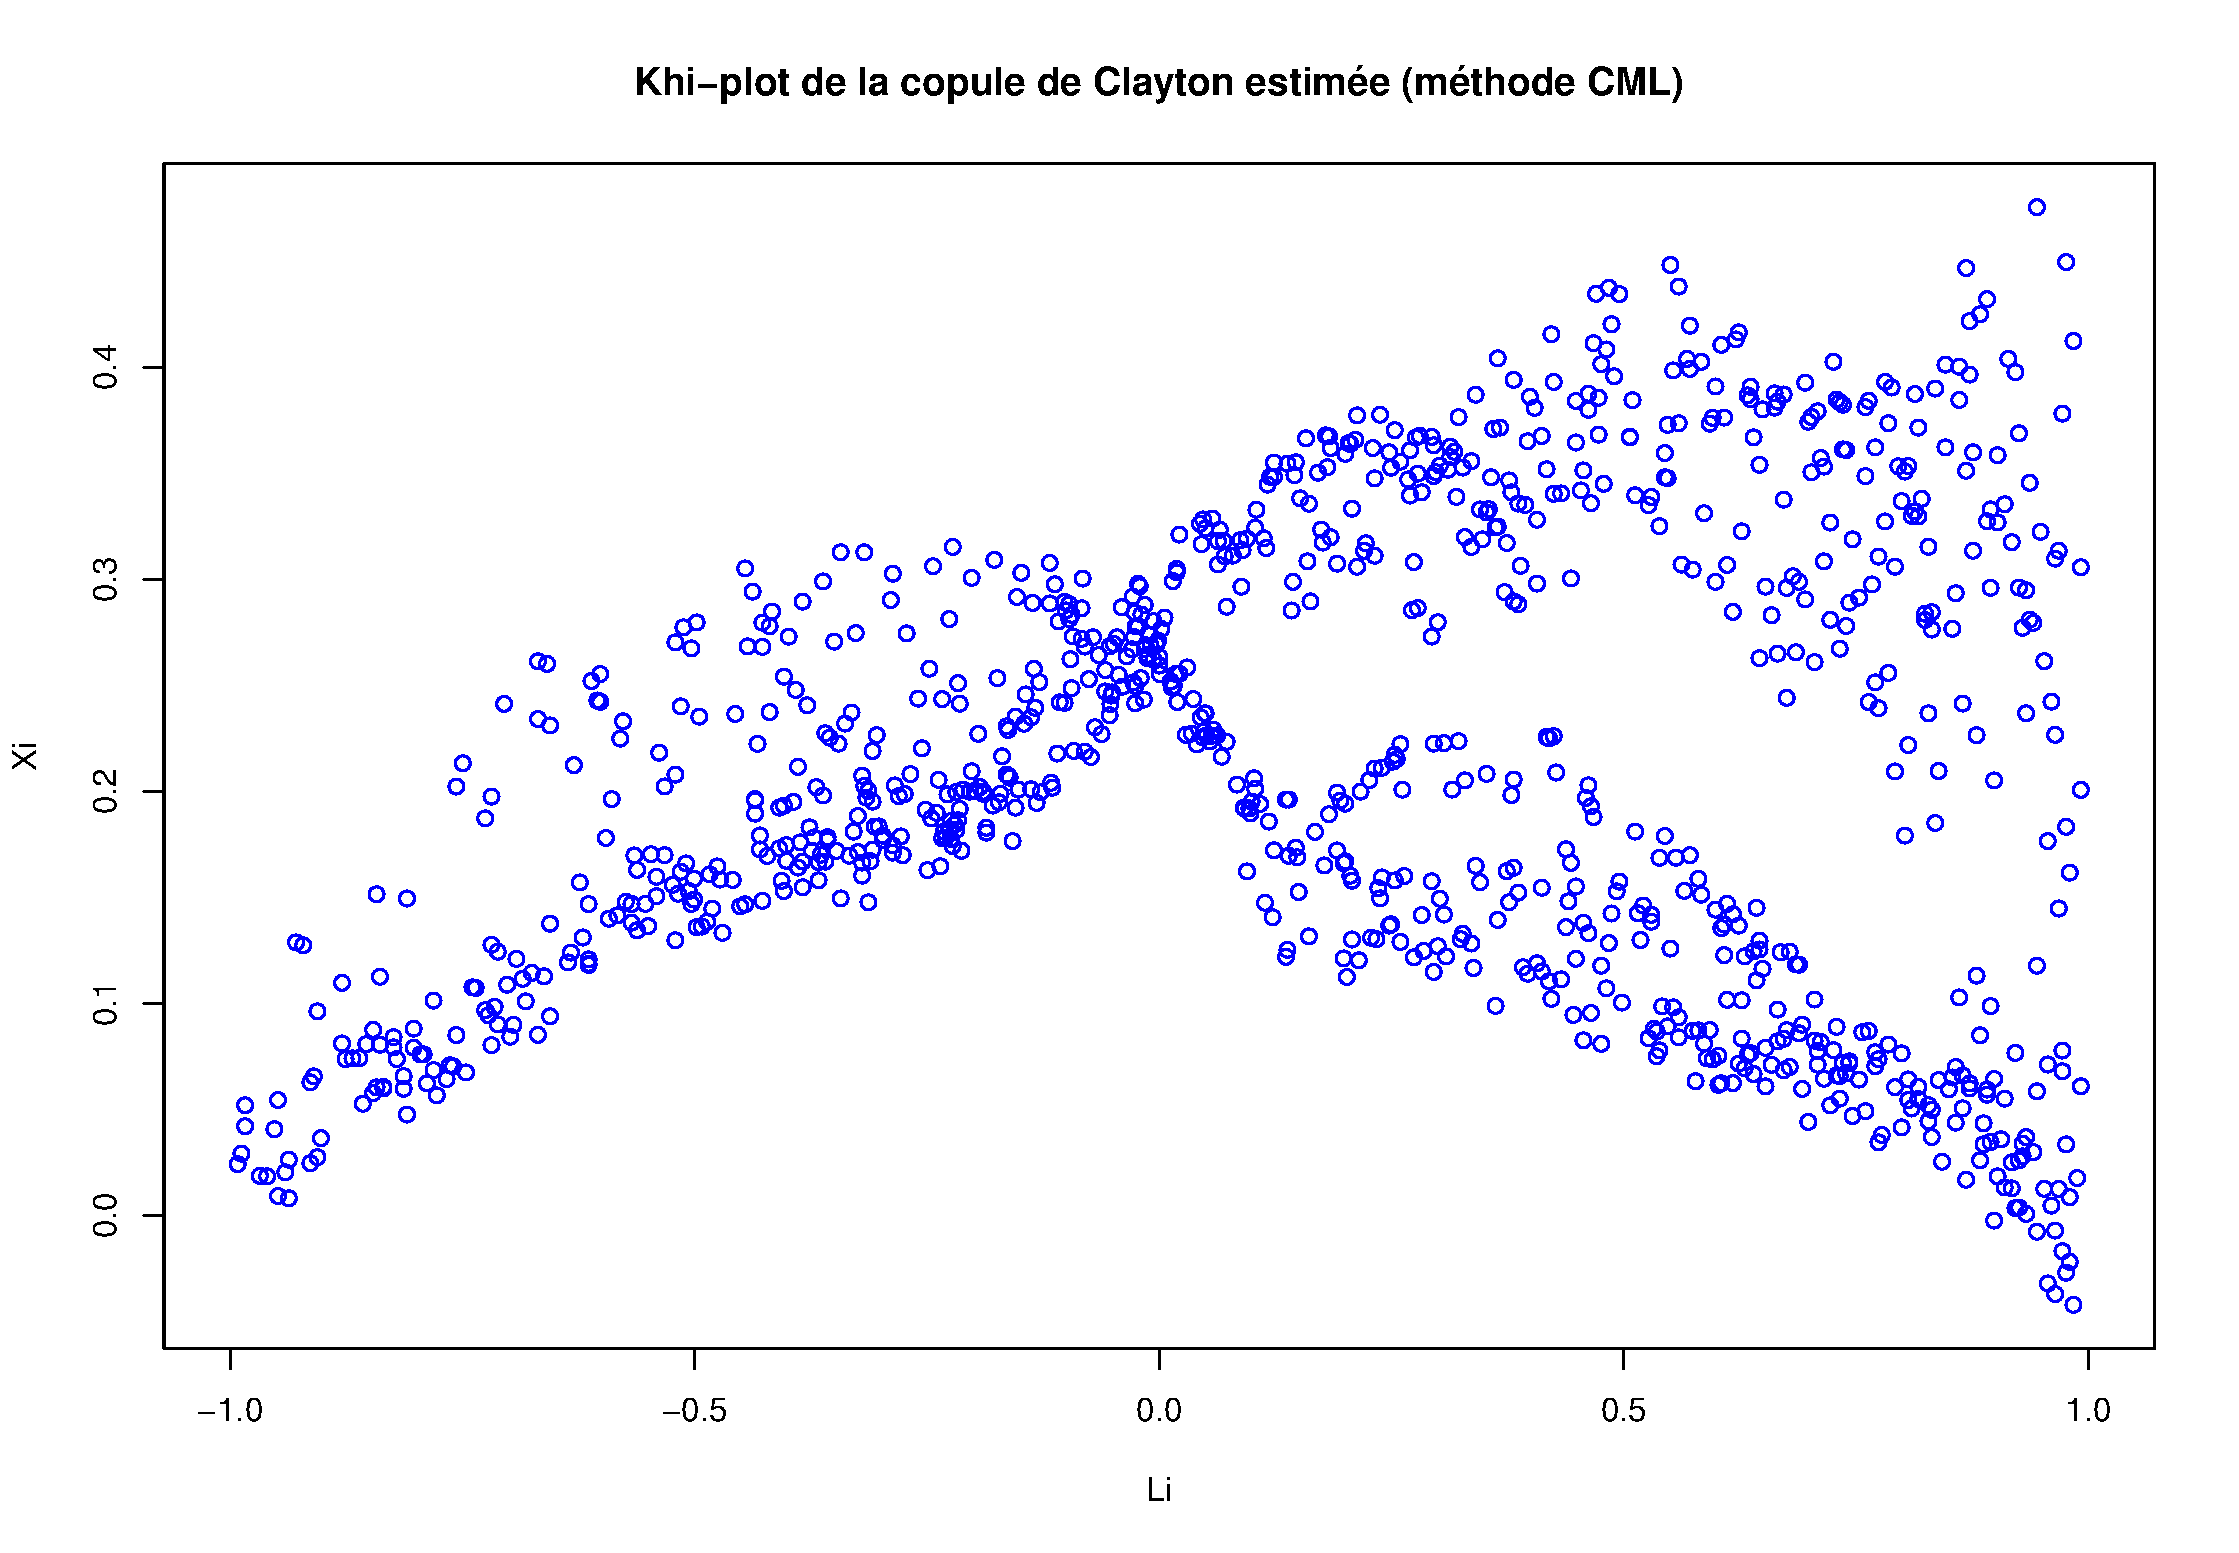
\includegraphics[width=17 cm, angle=0]{./pictures/claytoncmlkhiplot.png}
      \centering\caption{\label{2}Khi-plot de la copule de Clayton estimée (méthode CML)}
    \end{center}
\end{figure}

En comparant ce graphe du Khi-plot avec celui obtenu pour la copule empirique, on peut apercevoir une ressemblance, notamment dûe au fait que les points se répartissent du même côté de l'axe des ordonées (du côté positif) exprimant ainsi une dépendance positive. Cependant, du côté positif de l'axe des abscisses, le nuage de point semble se séparer en deux. Ceci n'est pas observée sur le Khi-plot de la copule empirique. 

\noindent%
\begin{figure}[H]
    \begin{center}
      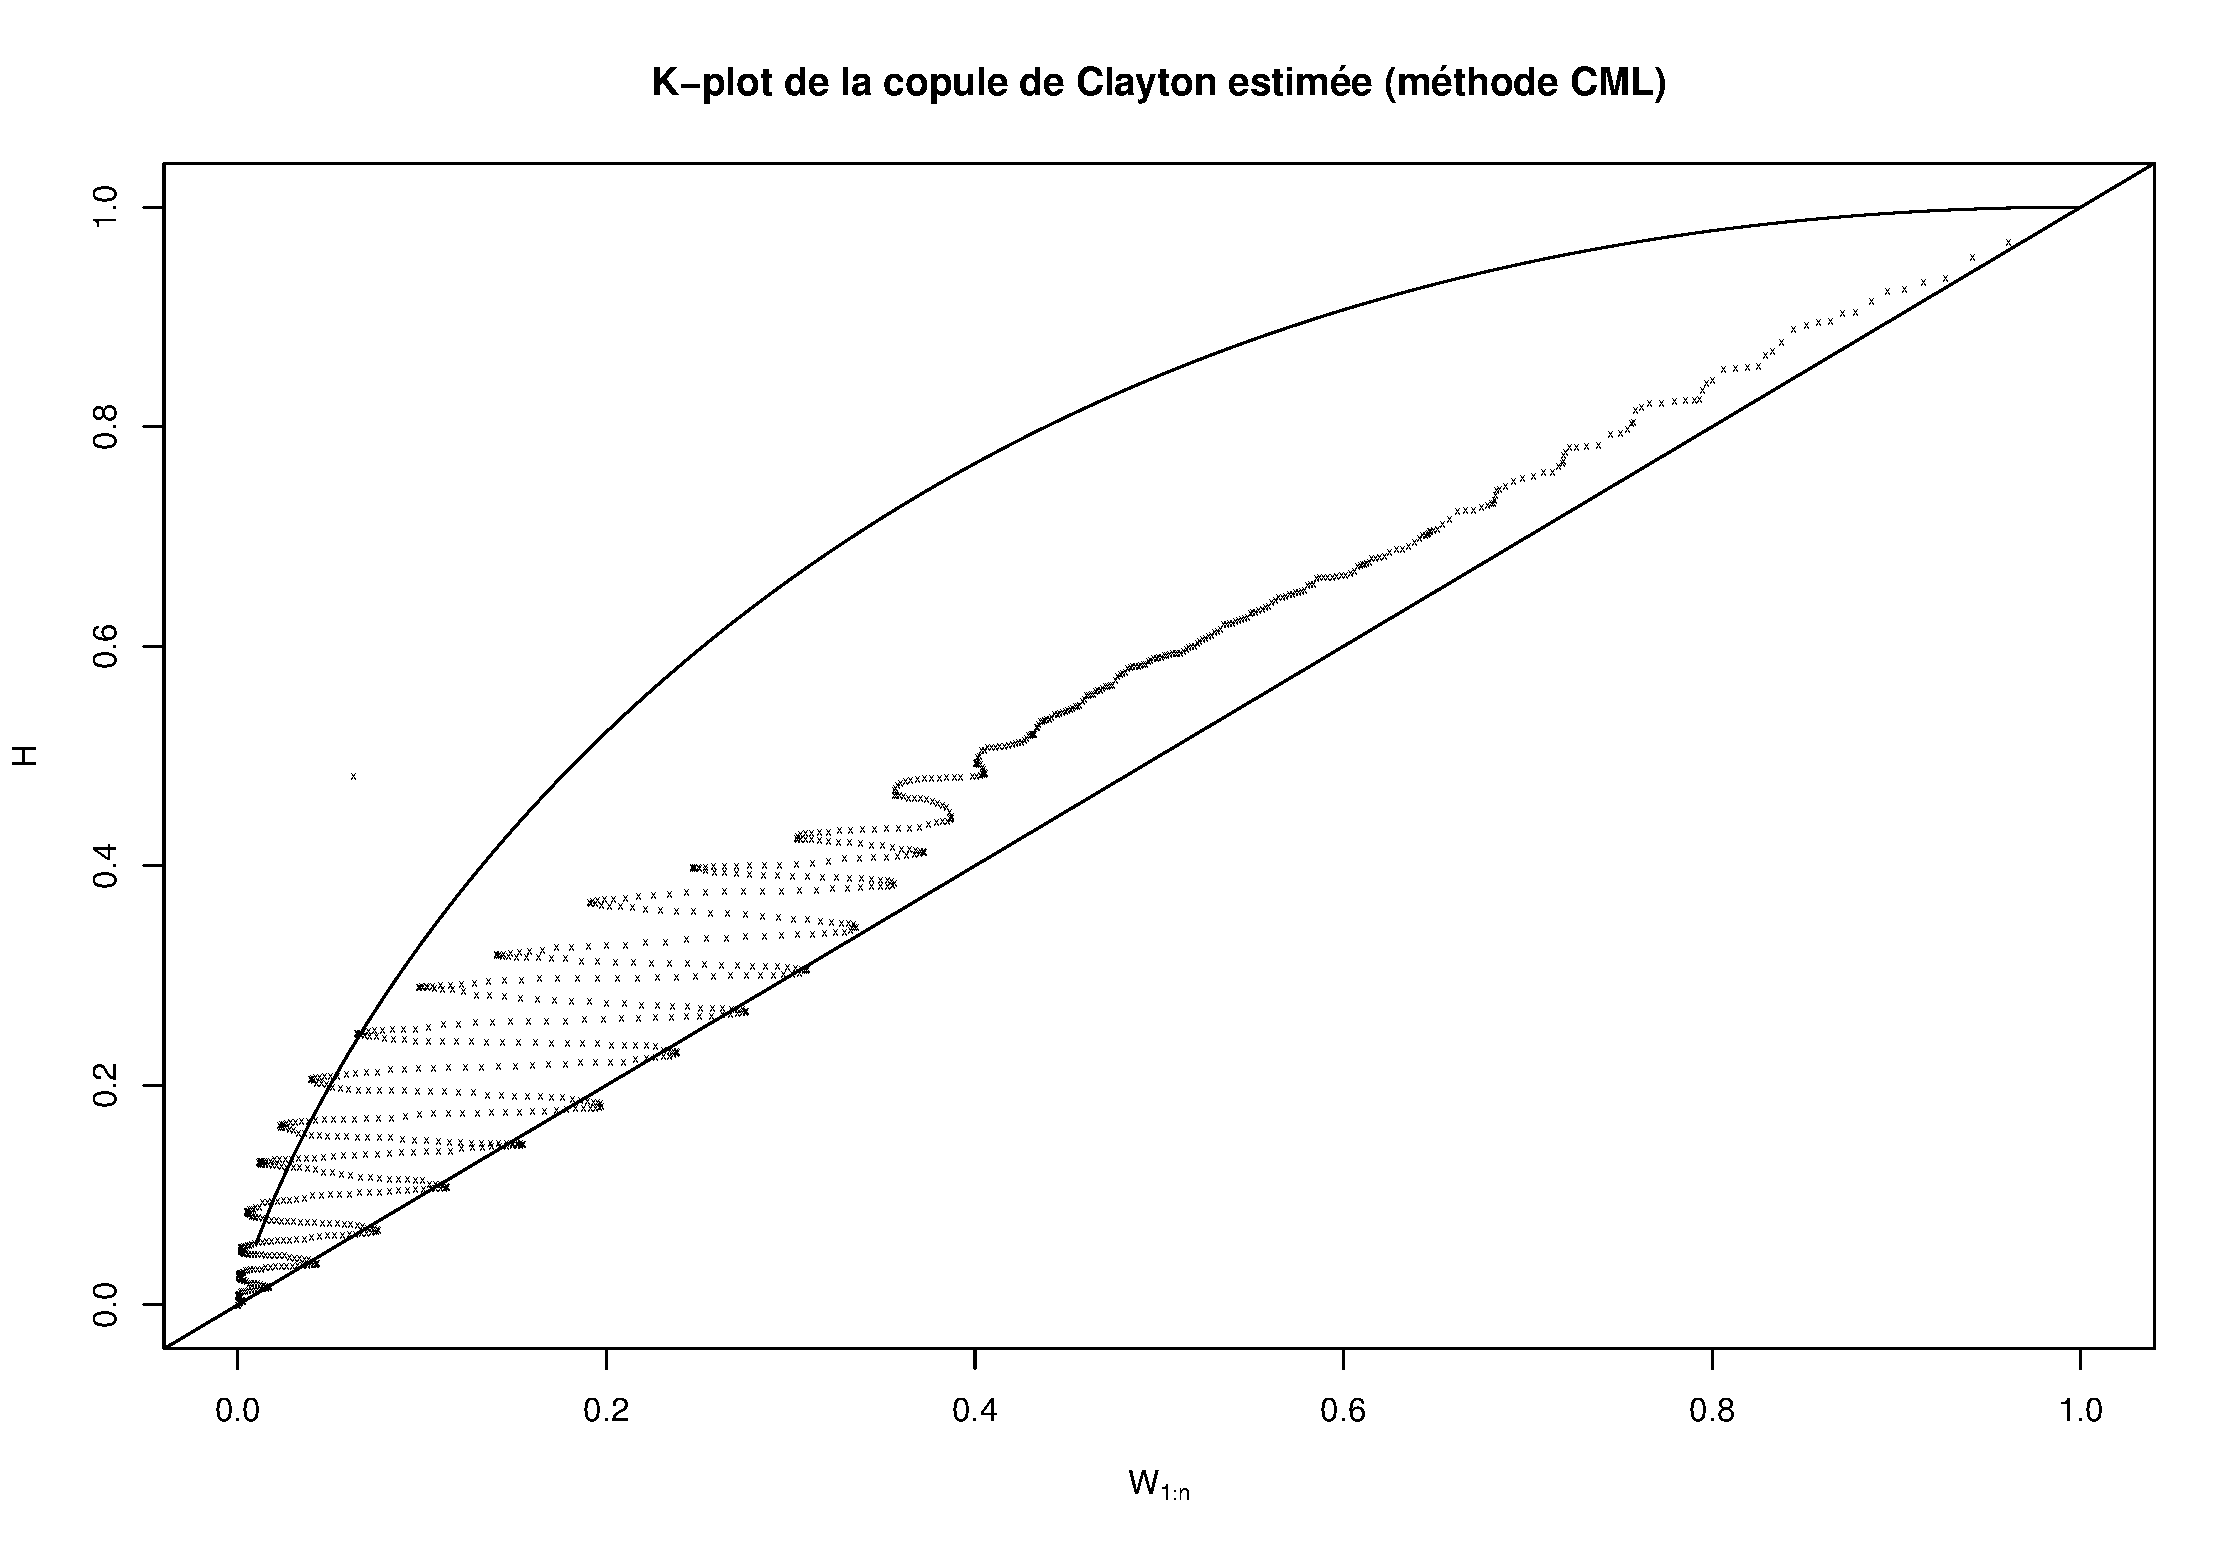
\includegraphics[width=17 cm, angle=0]{./pictures/claytoncmlkplot.png}
      \centering\caption{\label{2}K-plot de la copule de Clayton estimée (méthode CML)}
    \end{center}
\end{figure}

De la même manière, pour ce graphe du K-plot, on observe une similitude et plusieurs disparités par rapport à celui de la copule empirique. En effet, les points semblent se répartir dans le même espace pour les deux figures (globalement entre la courbe de dépendance positive parfaite et la droite d'indépendance $y=x$). Cela montre une nouvelle fois la dépendance positive entre nos deux séries de données. Cependant, concernant le graphe associé à la copule de Clayton estimée, les variations de la répartition des points sont plus grandes et plus nombreuses. Certains points dépassent en effet la courbe de dépendance positive parfaite et on compte également $14$ oscillations distinctes contre $12$ pour le K-plot de la copule empirique. De plus, pour les espérances de la statistique d'ordre des rangs les plus élevés, les points se rapprochent de la droite $y=x$ alors qu'ils sont proches de la courbe de dépendance positive parfaite pour le graphe concernant la copule empirique.

Ces graphes du Khi-plot et K-plot sont donc d'une certaine façon assez éloignés de ceux obtenus pour la copule empirique.

Pour prolonger nos résultats, on réalise également un algorithme de bootstrap paramétrique. Il s'agit de tester l'adéquation à notre modèle de copule. L'hypothèse nulle du test est donc la suivante:
$$
H_0 : C \in (C_{\theta})
$$
Avec $C_{\theta}$ la famille des copules de Clayton dans notre cas. 
En utilisant les mêmes notations que dans le cours, on rejette l'hypothèse nulle si $D_n > L$. 
Dans notre situation, on obtient, avec un seuil de $0,05$, $D_n = 0,1340 > 0,0463 = L$. De plus, la p-value pour cette statistique de Cramer-Von Mises vaut $0$. Avec la fonction \textit{gofCopula} de R, on obtient une p-value de $0,0004$. 
Nous signalons que nous avons codé nous-mêmes l'algorithme du bootstrap paramétrique, la fonction \textit{gofCopula} de R nous permet seulement de vérifier les résultats de notre algorithme.
La copule empirique ne fait donc pas partie de la famille des copules de Clayton.

En conclusion de cette étude sur la copule de Clayton estimée, on peut considérer que la modélisation de la dépendance entre nos deux séries de données par une copule de Clayton n'est pas satisfaisante.

\subsection{Copule de Gumbel}

On procède de la même manière que pour la copule de Clayton. On obtient en sortie de l'algorithme une valeur de $\widehat{\theta}_{CML}=1,4699$ comme estimation du paramètre de la copule de Gumbel par la méthode CML. On a également la valeur de l'écart type $sd = 0,0561$. L'estimation obtenue est ainsi significative. Le maximum de vraisemblance vaut $94,3$.

On représente ainsi ci-dessous les graphes du Khi-plot et du K-plot de la copule de Gumbel estimée:

\noindent%
\begin{figure}[H]
    \begin{center}
      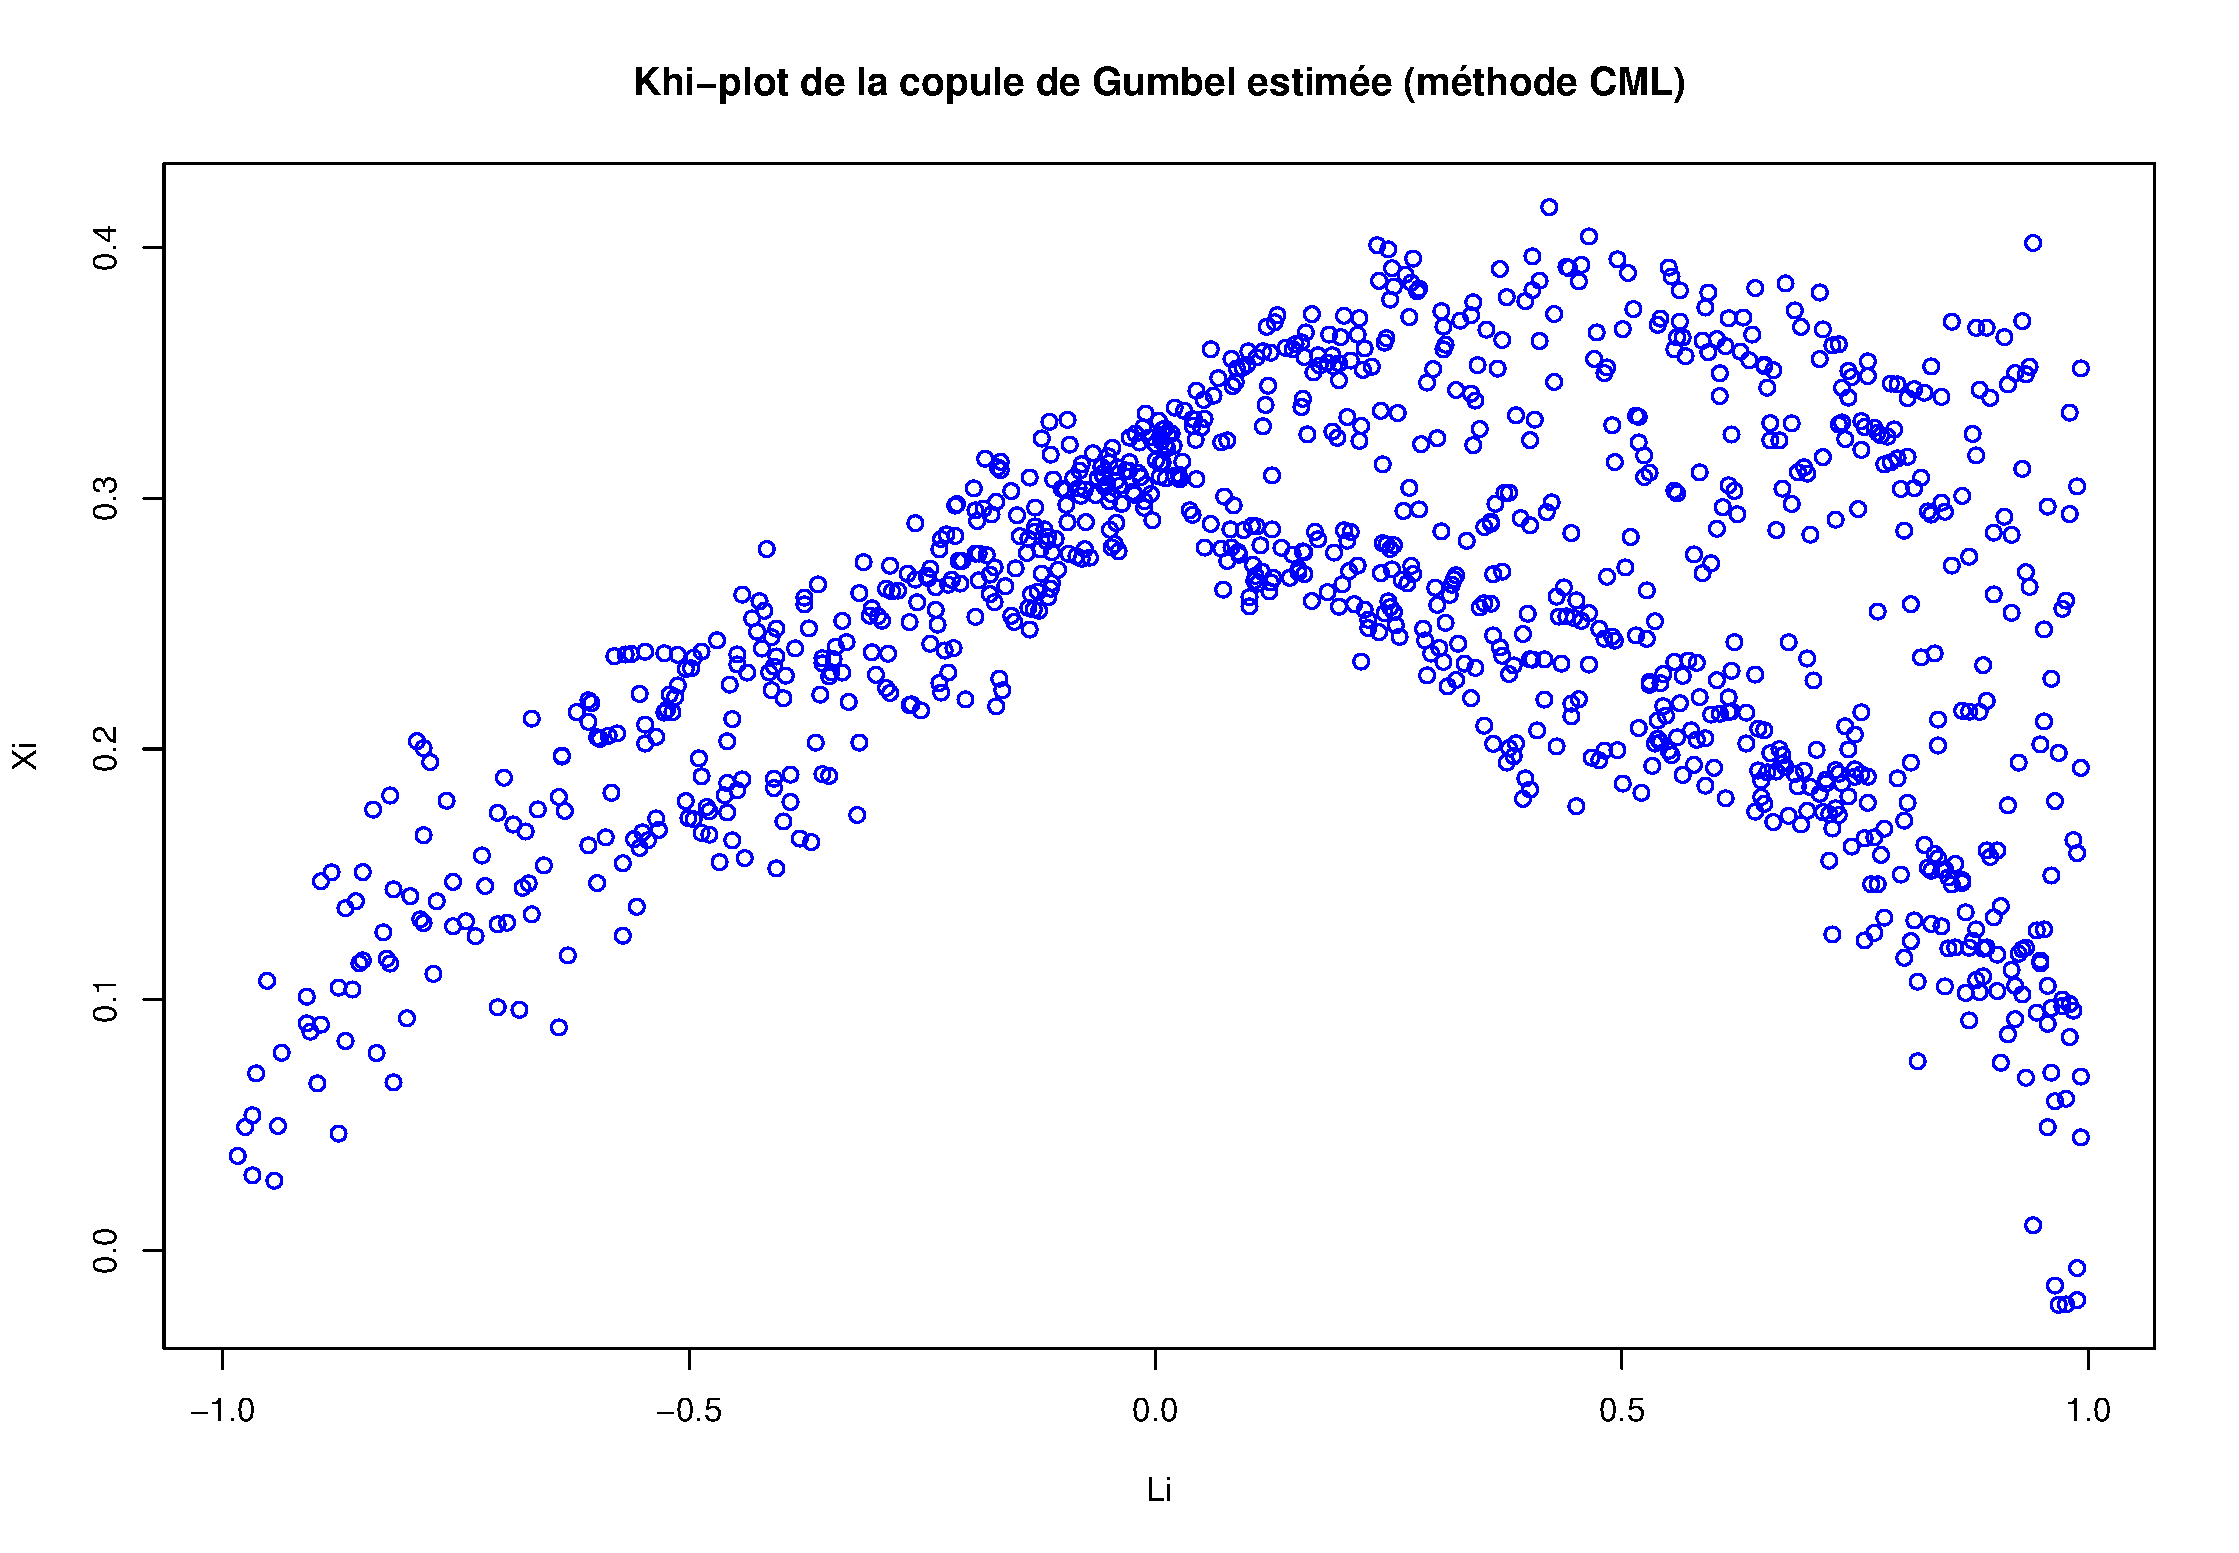
\includegraphics[width=17 cm, angle=0]{./pictures/gumbelcmlkhiplot.png}
      \centering\caption{\label{2}Khi-plot de la copule de Gumbel estimée (méthode CML)}
    \end{center}
\end{figure}

Le Khi-plot ci-dessus est très proche du Khi-plot obtenu avec la copule empirique. En effet, nous avons une répartition des points semblables. Le nuage de points est incurvée de la même manière du coté des valeurs positives des ordonnées et atteint une valeur maximale autour de $0,3$ comme pour le Khi-plot empirique. Certes, nous avons toujours une sorte de séparation en deux du nuage de points pour les valeurs positives en abscisse. Mais, cela est beaucoup moins prononcé que pour le Khi-plot de la copule de Clayton précédent.

\noindent%
\begin{figure}[H]
    \begin{center}
      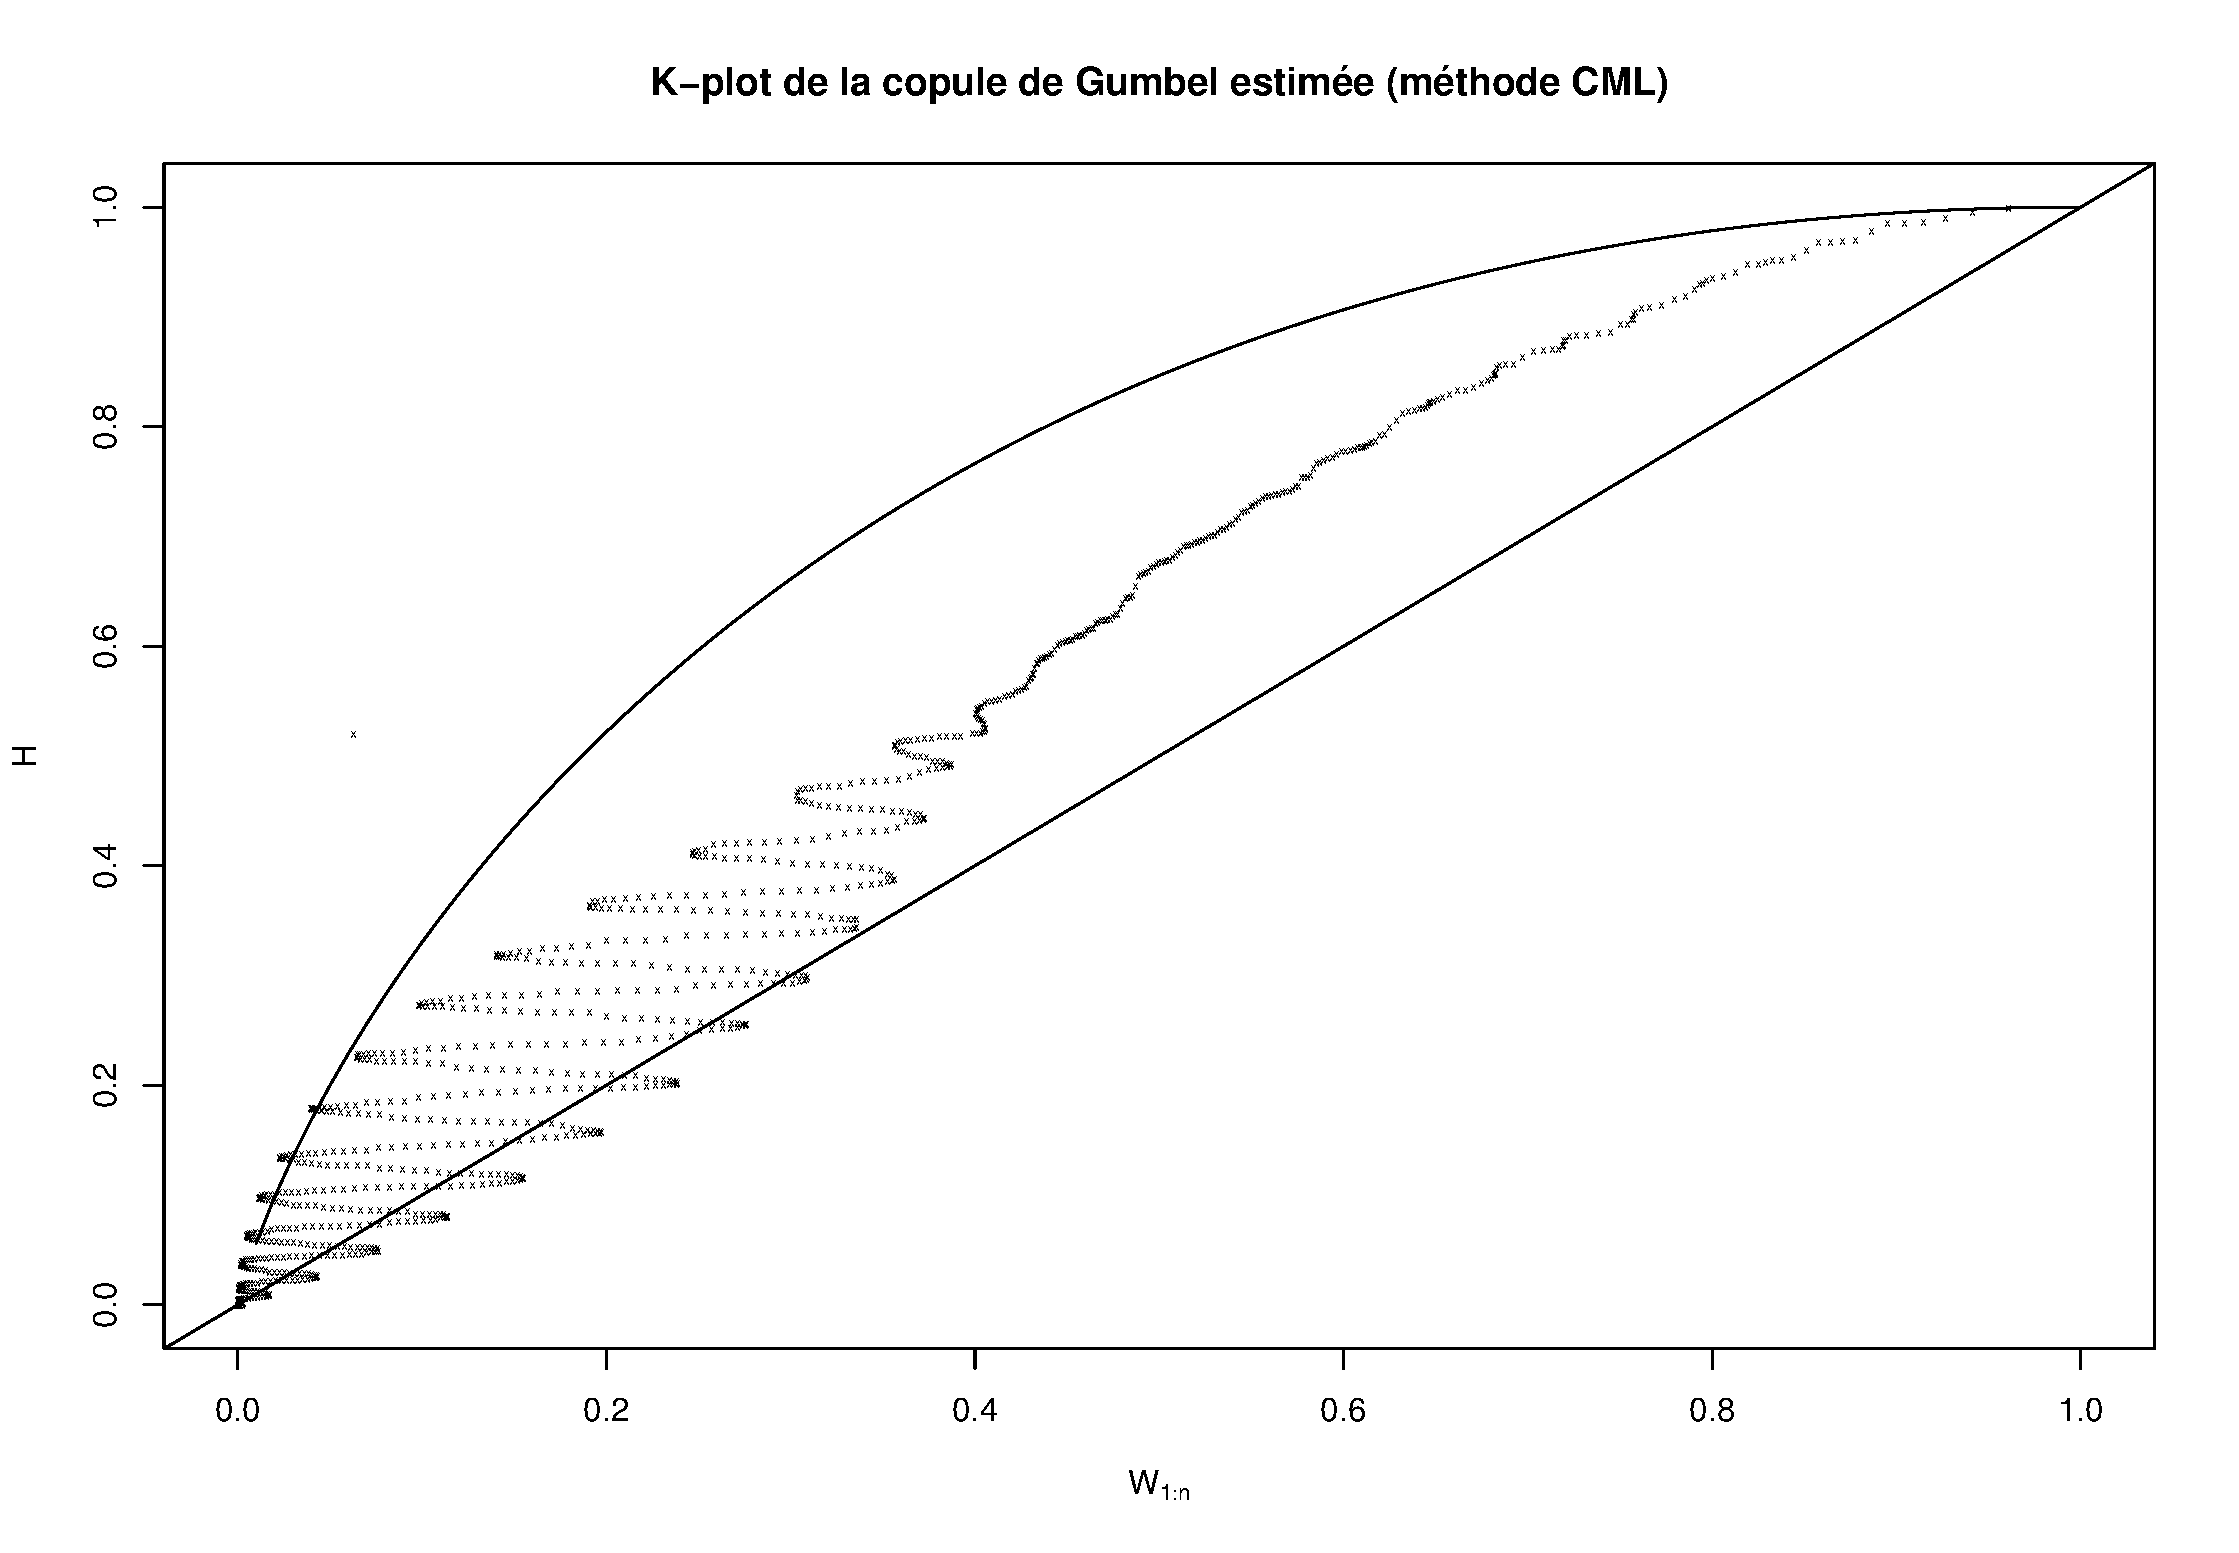
\includegraphics[width=17 cm, angle=0]{./pictures/gumbelcmlkplot.png}
      \centering\caption{\label{2}K-plot de la copule de Gumbel estimée (méthode CML)}
    \end{center}
\end{figure}

Le K-plot de la copule de Gumbel estimée et celui de la copule empirique sont très proches. Les points se répartissent dans le même endroit du graphe (entre la droite $y=x$ et la courbe de dépendance positive parfaite). De plus, on compte le même nombre d'oscillations distinctes ($12$) et les espérances de la statistique d'ordre des rangs les plus élevés sont très proches de la courbe de dépendance positive parfaite pour les deux graphes. 

Les deux graphes précédents semblent donc concordants avec les graphes de la copule empirique.
Cependant, en appliquant l'algorithme du bootstrap paramétrique, on obtient, pour un seuil de 0,05, $D_n = 0,0412 > 0,0325 = L$. On obtient une p-value de $0,01$. Avec la fonction \textit{gofCopula} de R, on obtient une p-value de $0,01249$. 
Nous signalons que nous avons codé nous-mêmes l'algorithme du bootstrap paramétrique, la fonction \textit{gofCopula} de R nous permet seulement de vérifier les résultats de notre algorithme.
Ainsi, on rejette l'hypothèse nulle et on ne peut pas conclure que notre copule empirique fasse partie de la famille des copules de Gumbel.

Ce dernier résultat sur la copule de Gumbel estimée n'est donc pas satisfaisant, alors même qu'il s'agit de la famille de copules qui a été choisie dans le papier de Dutang et Charpentier. Ainsi, nous pouvons voir si d'autres copules peuvent encore mieux s'approcher de la copule empirique.

\subsection{Copule de Frank}

L'estimation du paramètre de la copule de Frank par méthode CML est $\widehat{\theta}_{CML}=3,1729$. L'écart type obtenu est plus élevé que pour les deux études précédentes mais l'estimation reste largement significative. On a $sd = 0,2781$. Le maximum de vraisemblance est égal à $76,04$. Avec cette estimation, nous pouvons simuler des données issues d'une copule de Frank ayant cette valeur de paramètre. On obtient alors les graphes du Khi-plot et K-plot de la copule de Frank estimée ci-dessous:

\noindent%
\begin{figure}[H]
    \begin{center}
      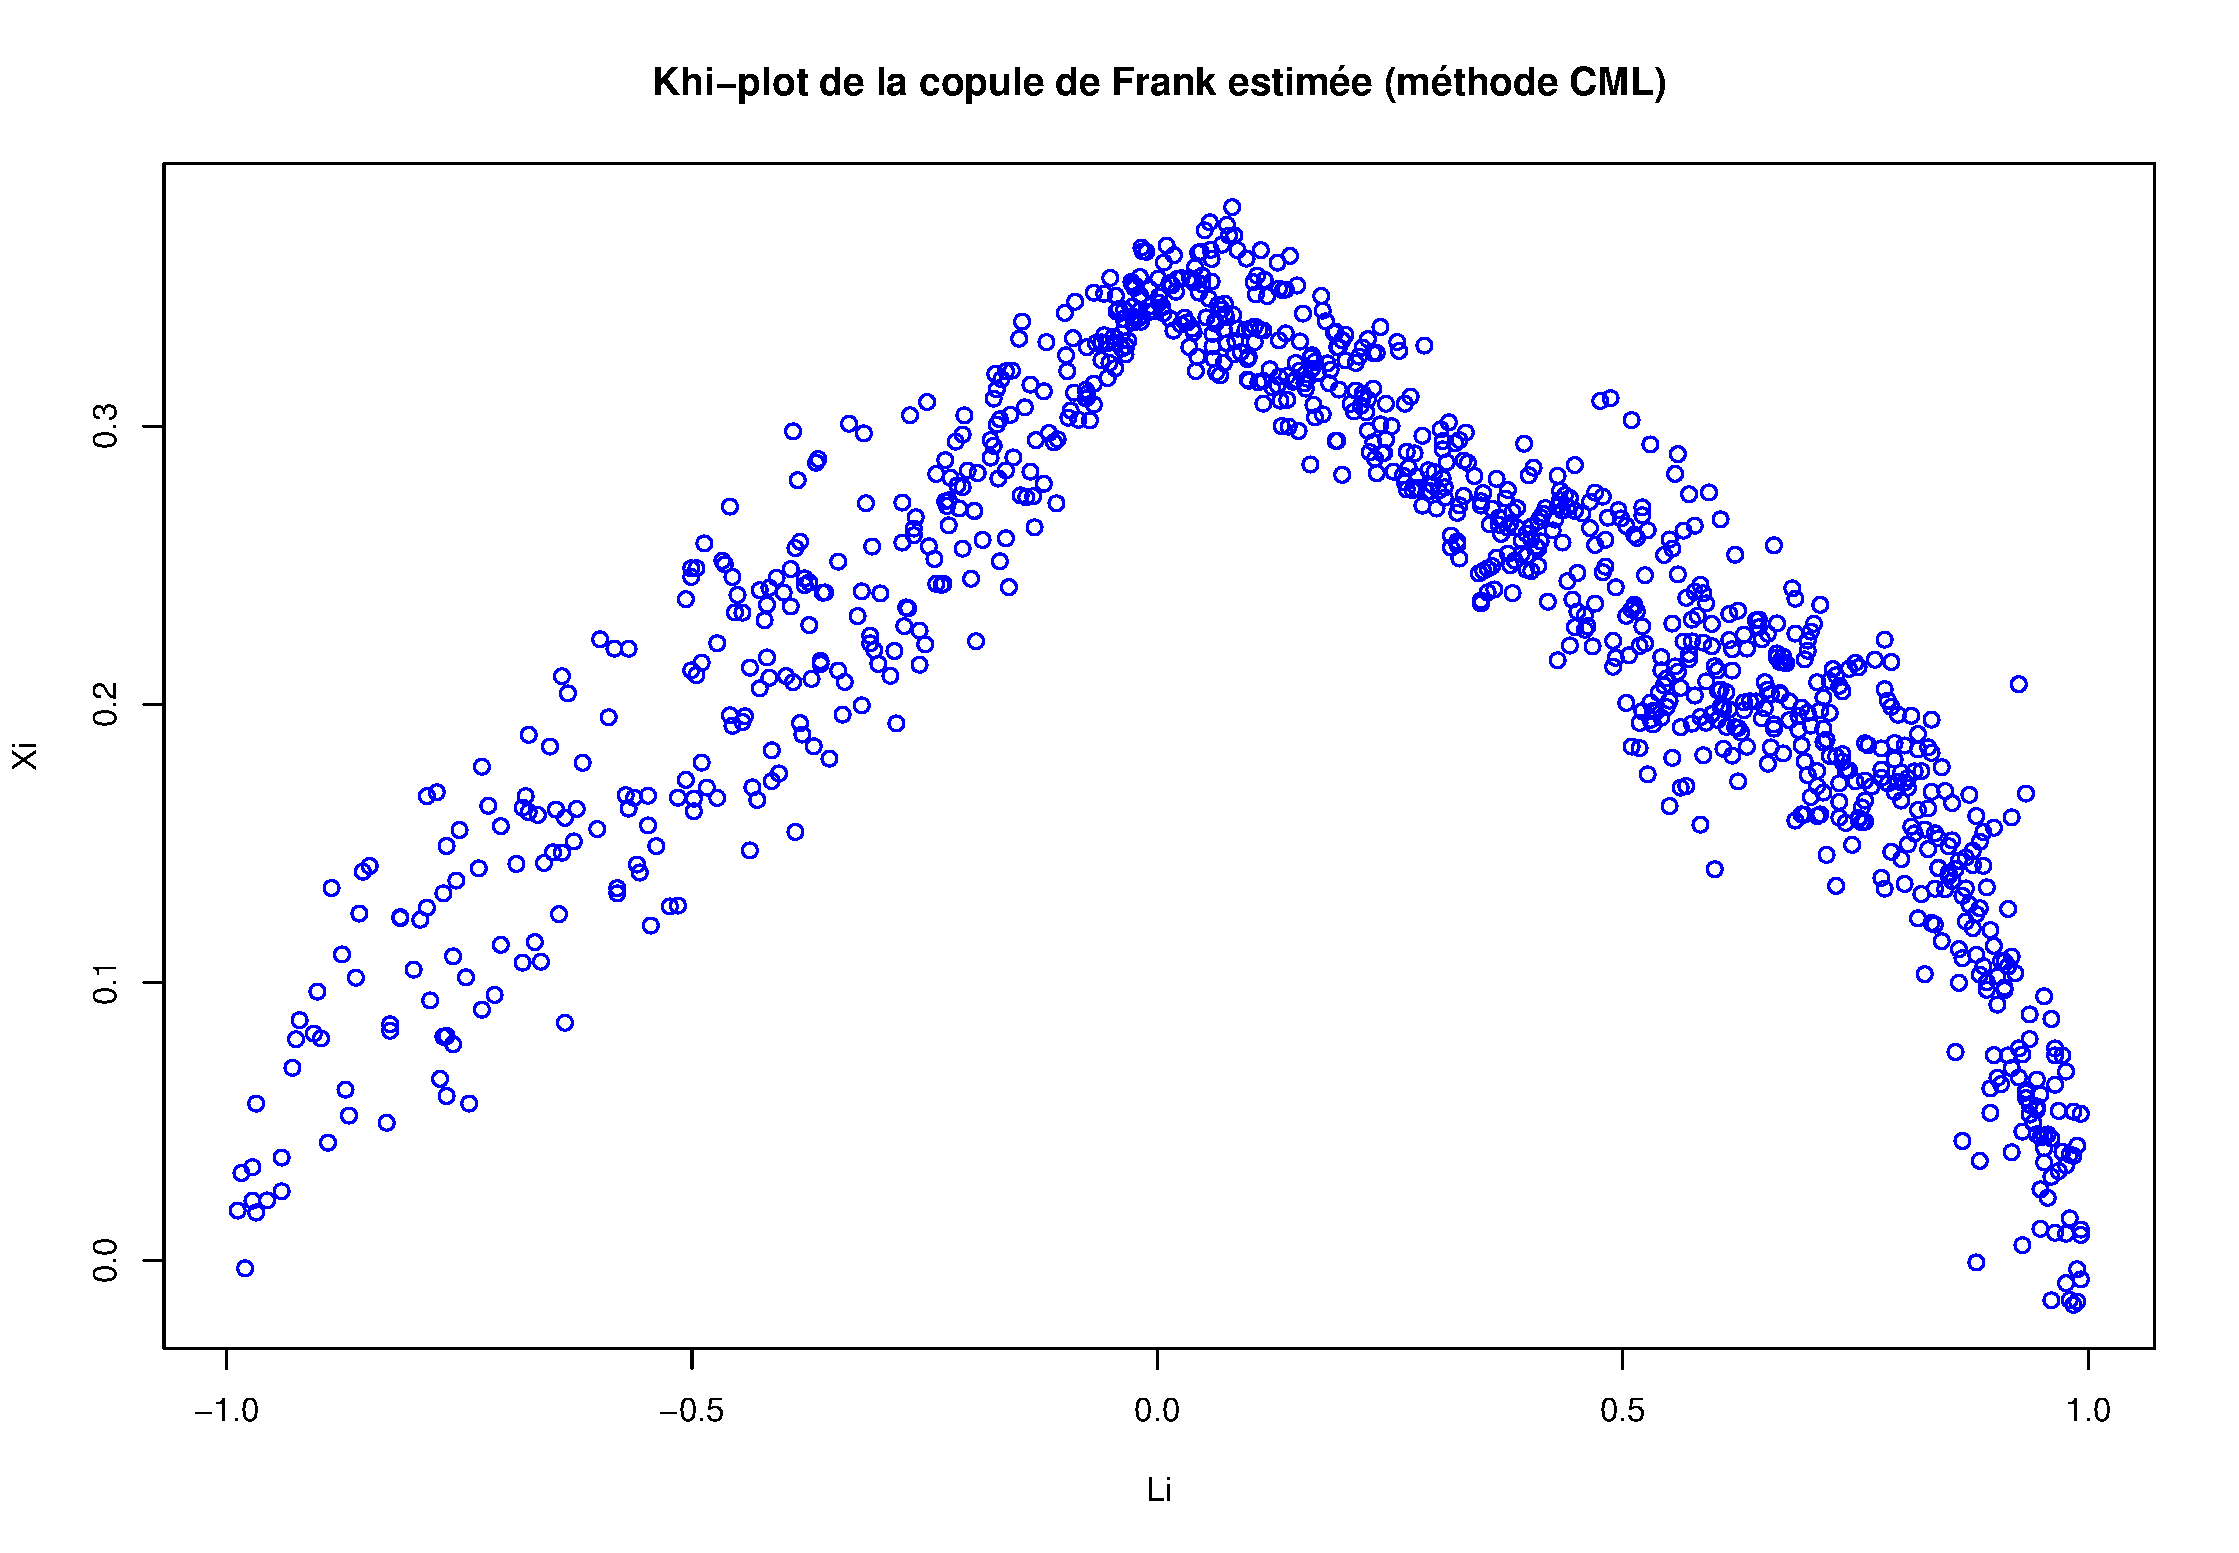
\includegraphics[width=17 cm, angle=0]{./pictures/frankcmlkhiplot.png}
      \centering\caption{\label{2}Khi-plot de la copule de Frank estimée (méthode CML)}
    \end{center}
\end{figure}

Bien que la forme du graphe ci-dessus soit proche de celui effectué pour la copule empirique, on peut remarquer plusieurs différences importantes. Tout d'abord, le Khi-plot de la copule de Frank estimée est beaucoup trop "pentu" par rapport à celui de la copule empirique. Les valeurs aux extrêmes ont une ordonnée autour de $0$ et le maximum en ordonnée dépasse les $0,3$ alors que, pour le graphe de la copule empirique, la valeur maximale en ordonnée est autour de $0,3$ et les valeurs aux extrêmes en abscisse sont autour de $0,1$.

\noindent%
\begin{figure}[H]
    \begin{center}
      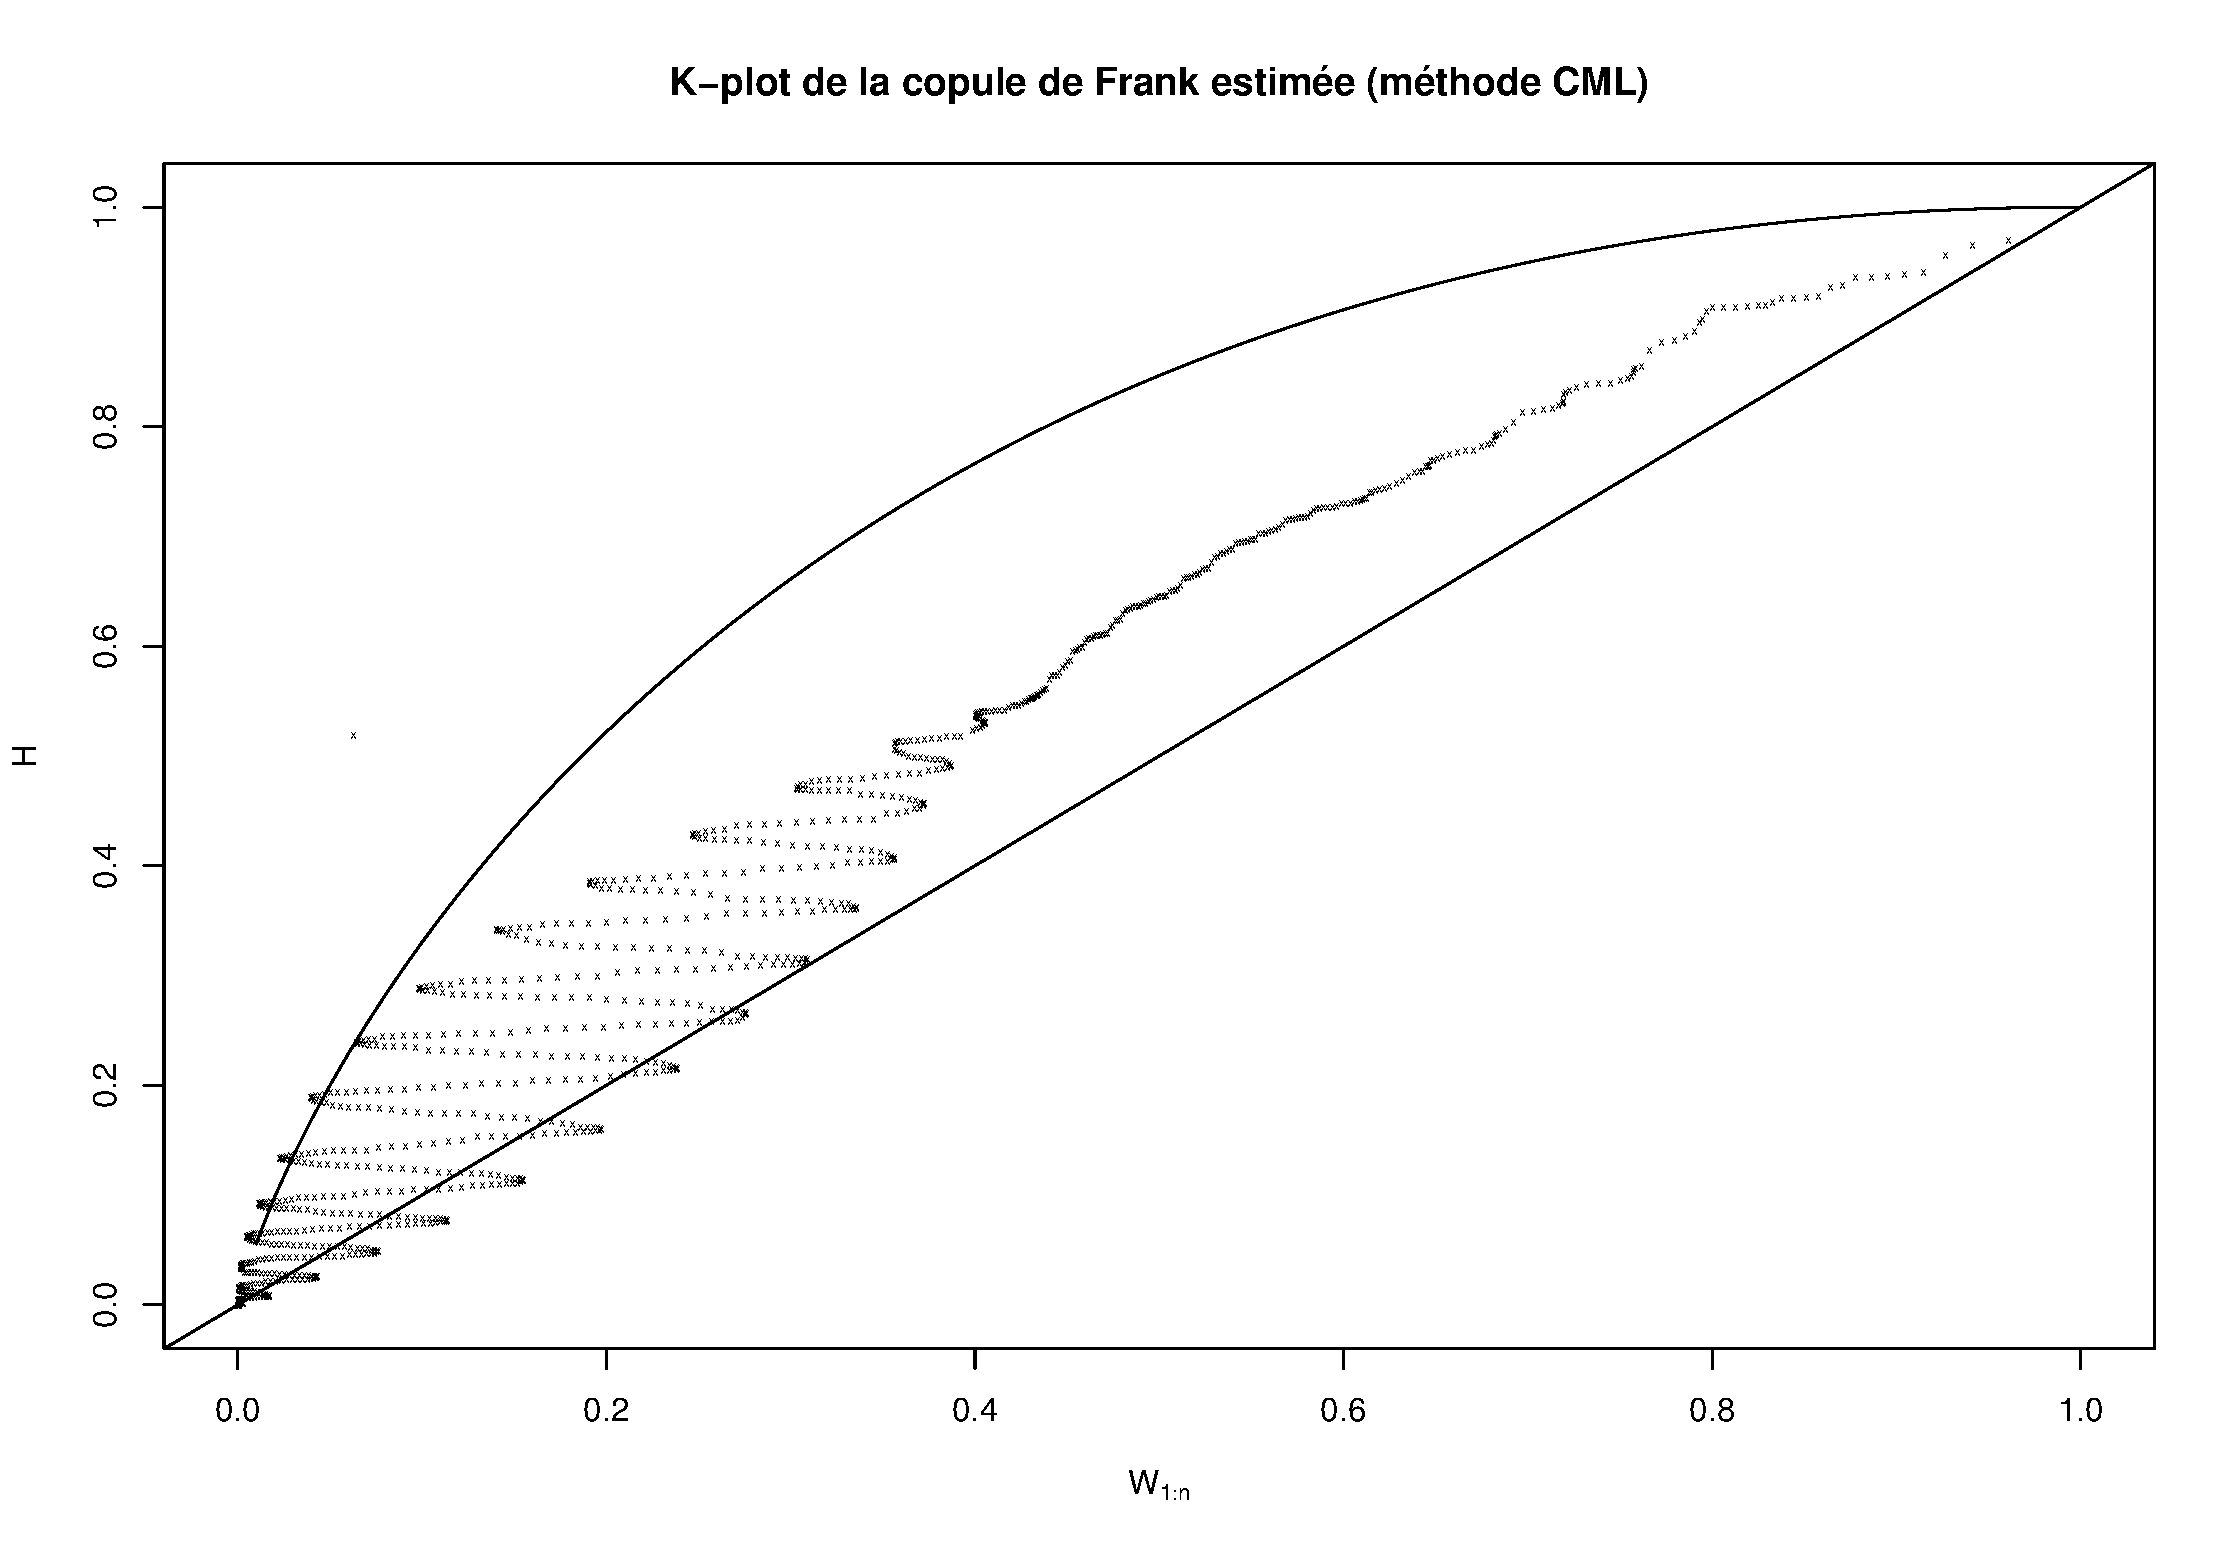
\includegraphics[width=17 cm, angle=0]{./pictures/frankcmlkplot.png}
      \centering\caption{\label{2}K-plot de la copule de Frank estimée (méthode CML)}
    \end{center}
\end{figure}

Le K-plot de la copule de Frank est assez similaire à celui de la copule de Clayton et présente donc les mêmes disparités par rapport à celui de la copule empirique. La différence la plus importante est que, pour les espérances de la statistique d'ordre des rangs les plus élevés, les points se rapprochent de la droite $y=x$ alors qu'ils sont proches de la courbe de dépendance positive parfaite pour le graphe concernant la copule empirique.

Ces graphes du Khi-plot et K-plot sont donc assez éloignés de ceux obtenus pour la copule empirique.

Cela est confirmé par l'algorithme du bootstrap paramétrique. On obtient $D_n = 0,050 > 0,025 = L$, pour un seuil de $0,05$. La p-value est nulle. Avec la fonction \textit{gofCopula} de R, on obtient une p-value de $0,0045$. 
Nous signalons que nous avons codé nous-mêmes l'algorithme du bootstrap paramétrique, la fonction \textit{gofCopula} de R nous permet seulement de vérifier les résultats de notre algorithme. 
Ainsi, on rejette l'hypothèse nulle et on conclut que la copule empirique ne fait pas partie de la famille des copules de Frank.

\subsection{Copule normale}

Par la méthode CML, on obtient l'estimation suivante du paramètre de la copule normale: $\widehat{\theta}_{CML}=0,51412$. L'écrat type associé vaut $sd = 0,031$, ce qui prouve la significativité de l'estimation obtenue. On obtient $94,83$ comme maximum de vraisemblance. 

Comme dans les études précédentes, on trace le Khi-plot et K-plot de la copule normale estimée et on les compare à ceux de la copule empirique.

\noindent%
\begin{figure}[H]
    \begin{center}
      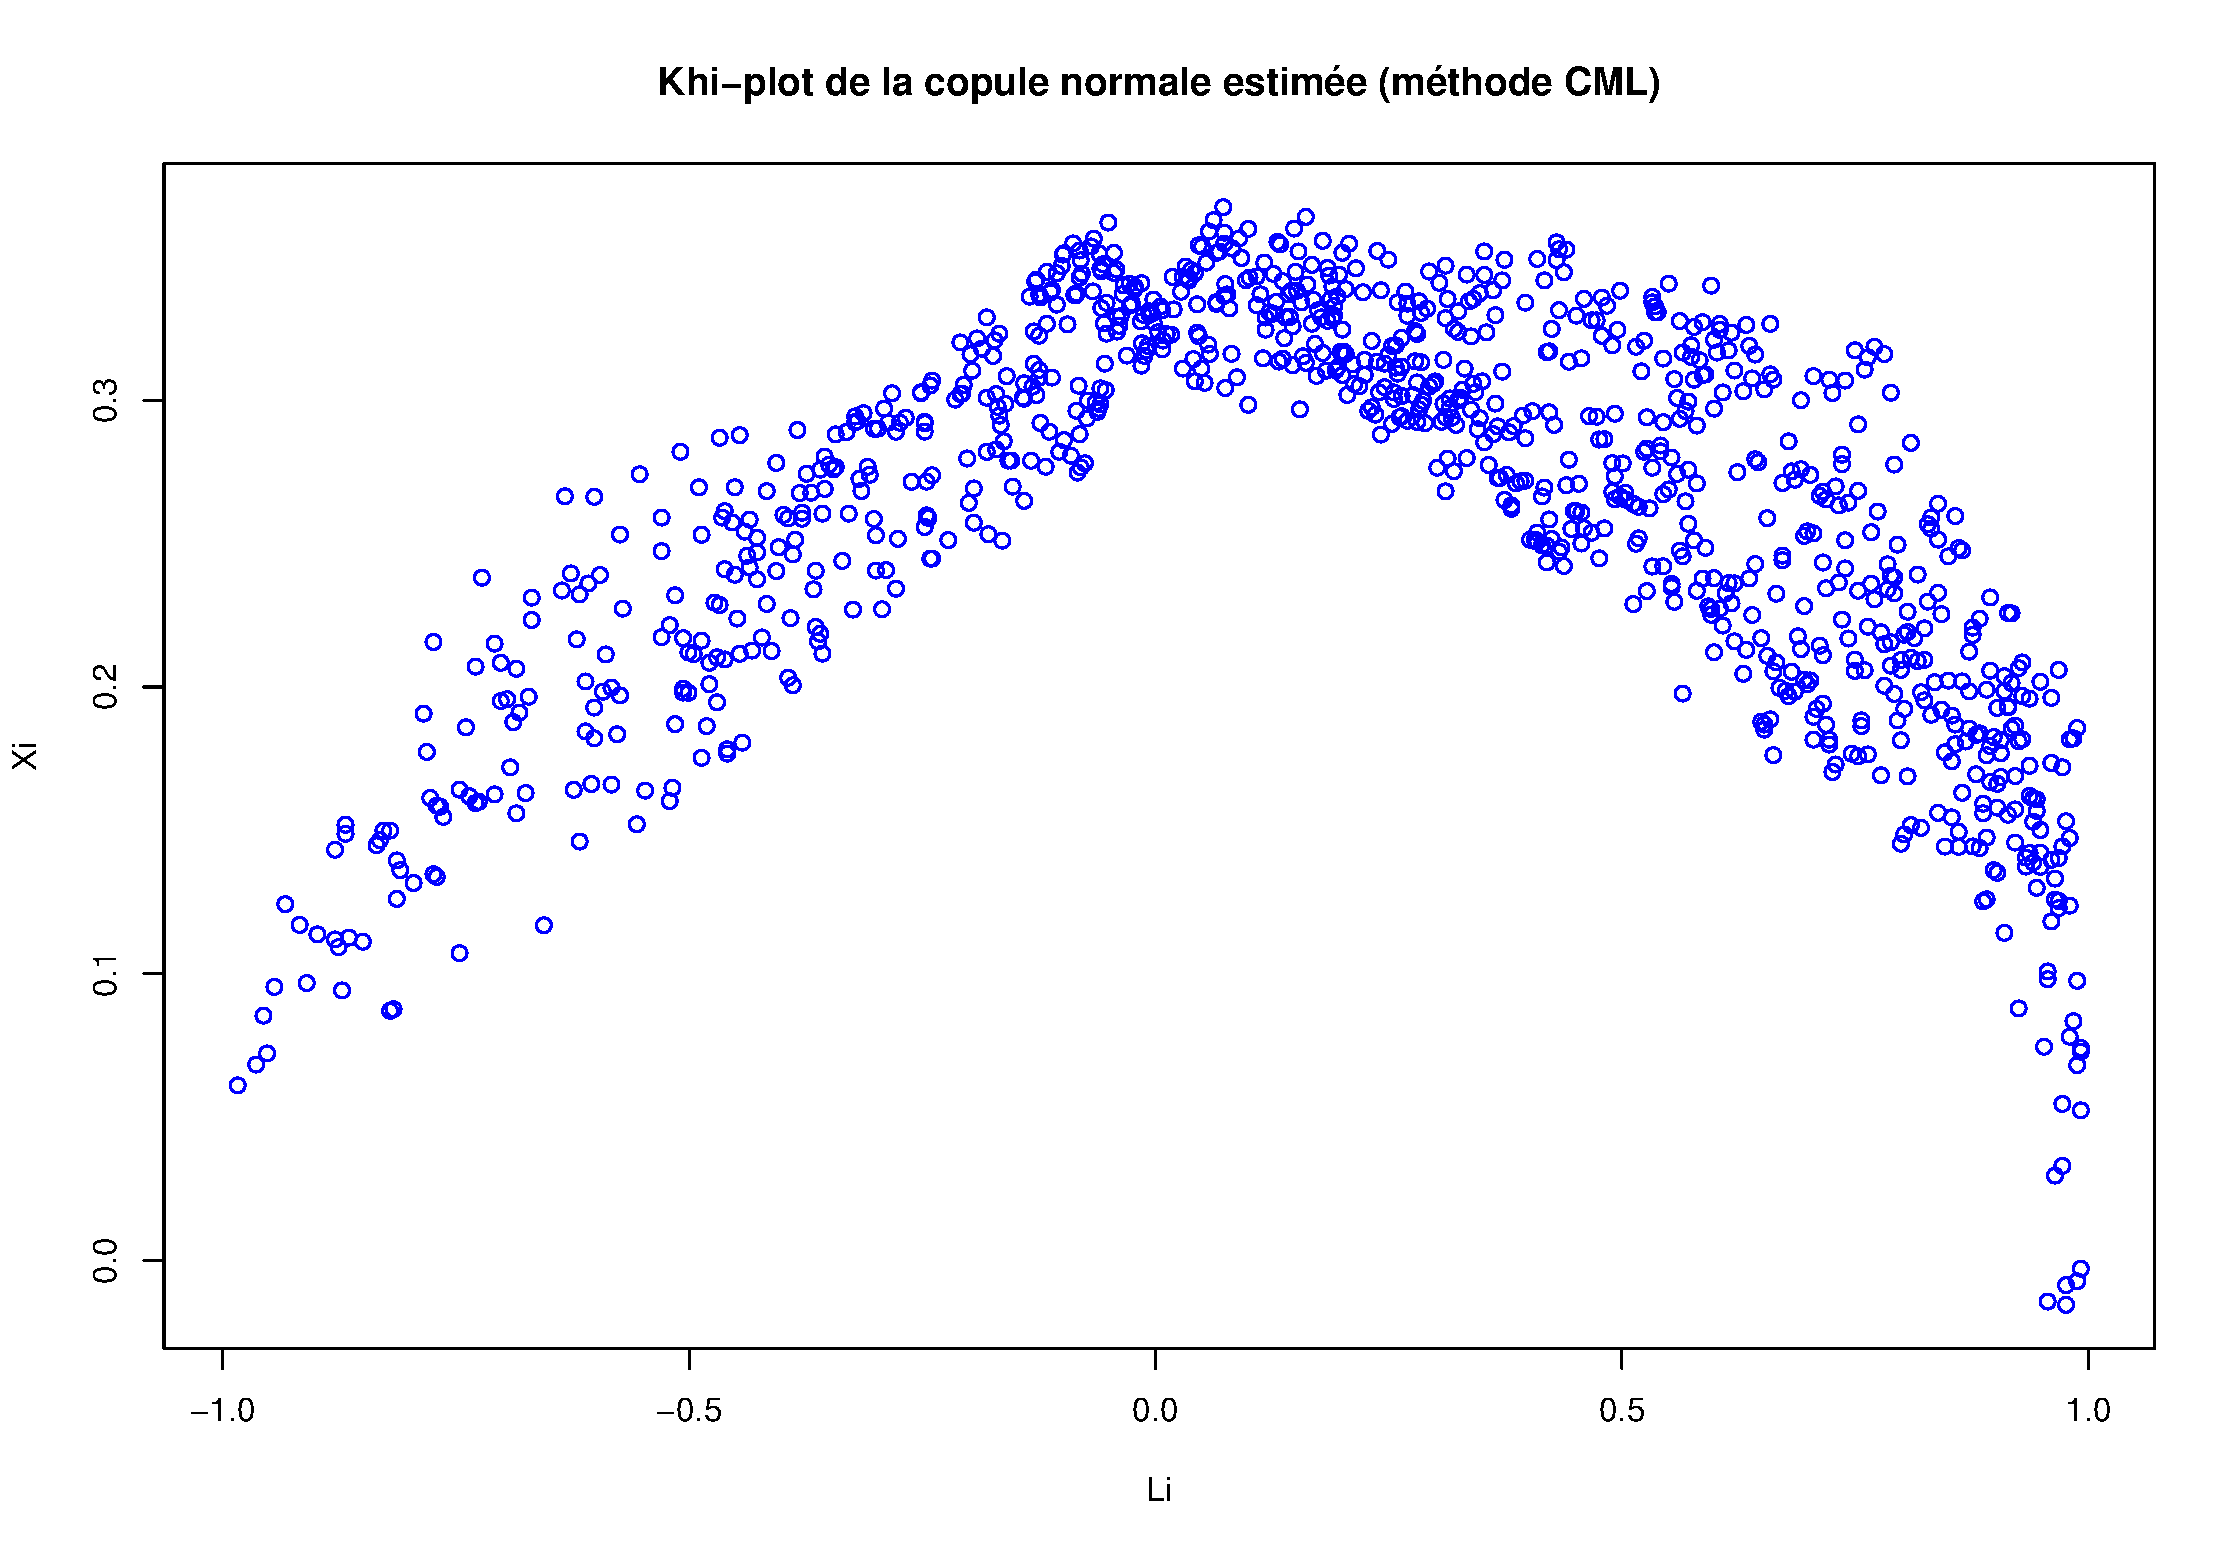
\includegraphics[width=17 cm, angle=0]{./pictures/normalcmlkhiplot.png}
      \centering\caption{\label{2}Khi-plot de la copule normale estimée (méthode CML)}
    \end{center}
\end{figure}

Le Khi-plot de la copule normale estimée est très proche de celui de la copule empirique. On retrouve, sur les deux graphes, la même forme globale du nuage de points. De plus, pour les deux, le maximum en ordonnée est autour de $0,3$ et les valeurs extrêmes des abscisses ont une ordonnée autour de $0,1$. 

\noindent%
\begin{figure}[H]
    \begin{center}
      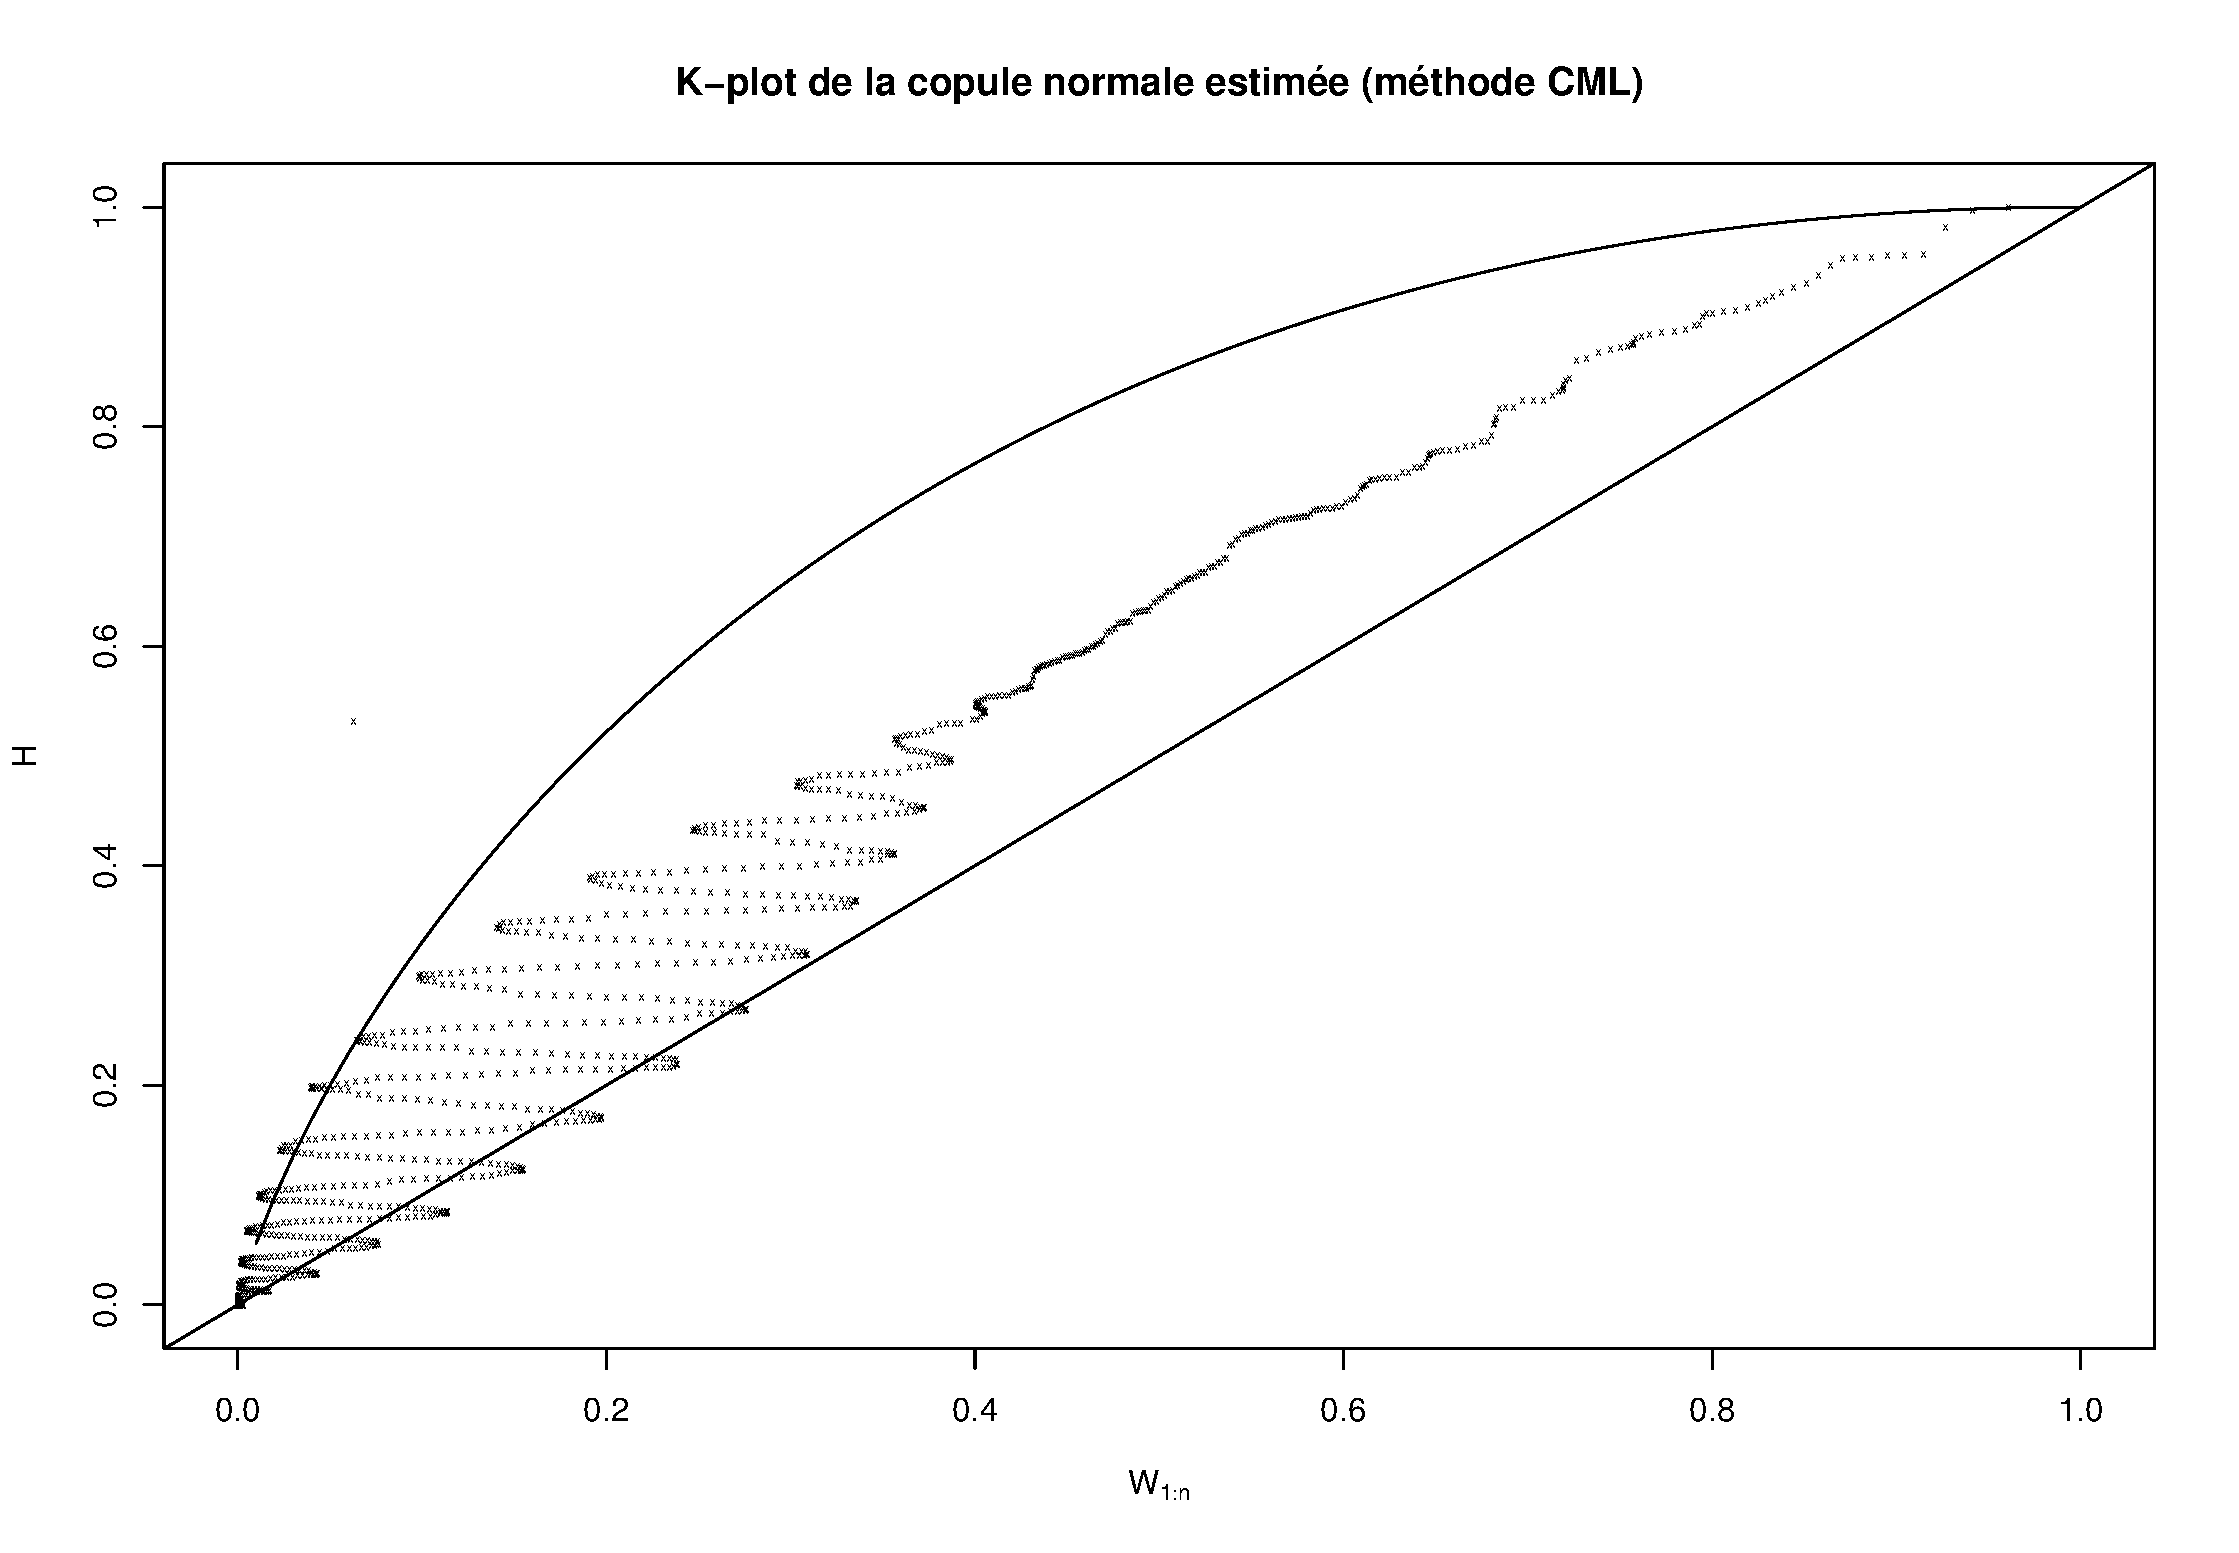
\includegraphics[width=17 cm, angle=0]{./pictures/normalcmlkplot.png}
      \centering\caption{\label{2}K-plot de la copule normale estimée (méthode CML)}
    \end{center}
\end{figure}

Concernant le K-plot de la copule normale estimée, il présente quelques différences avec celui associée à la copule empirique. En effet, les oscillations que l'on observe sont beaucoup plus fortes sur le K-plot de la copule normale estimée. De plus, pour ce K-plot, les espérances de la statistique d'ordre des rangs les plus élevés s'approchent de la courbe de dépendance positive maximale mais de façon plus atténuées que pour le K-plot de la copule empirique.

En résumé, bien que le Khi-plot de la copule normale soit très ressemblant avec celui de la copule empirique, le K-plot, lui, ne nous permet pas de conclure. L'algorithme du bootstrap paramétrique va ainsi nous permettre d'affirmer ou non si la copule empirique fait partie de la famille des copules normales. En sortie de cet algorithme, on a, pour un seuil de $0,05$, $D_n = 0,0314 < 0,0320 = L$. De plus, on obtient une p-value de $0,06$. Avec la fonction \textit{gofCopula} de R, on obtient une p-value de $0,05544$. 
Nous signalons que nous avons codé nous-mêmes l'algorithme du bootstrap paramétrique, la fonction \textit{gofCopula} de R nous permet seulement de vérifier les résultats de notre algorithme. 
On accepte ainsi l'hypothèse nulle et la copule empirique appartient bien à la famille des copules normales.

\subsection{Copule de Student}

\section{Méthode des moments}
%%%%%%%%%%%%%%%%%%%%%%%%%%%%%%%%%%%%%%%%%%%%%%%%%%%%%%%%%%%%%%%%%%%%%%%

Dans cette partie, nous utiliserons la méthode des moments pour estimer le paramètre des copules retenues afin de modéliser la dépendance entre les données sur Saint-Martin et celles sur Echirolles.

La méthode des moments utilise les relations existant entre le tau de Kendall (ou d'autres mesures de dépendance comme le rhô de Spearman) et les paramètres des
copules. Il est utilisé particulièrement lors de la détermination des paramètres des copules archimédiennes
et elliptiques en raison du déterminisme de certaines relations.

Pour les copules archimédiennes, le tau de Kendall $\tau$ est déterminé par :
$$
\tau = 1 + 4 \int_0^1 \frac{\phi(u)}{\phi'(u)}
$$
avec $\phi$ la fonction génératrice de la copule.

Pour la copule de Clayton, nous avons :
$$
\tau = 1 + 4 \int_0^1 \frac{\phi(u)}{\phi'(u)} = 1 + 4 \int_0^1 \frac{u^{-1} - 1}{-\theta u^{-\theta -1}} du = 1 + \frac{4}{\theta} \int_0^1 (u^{\theta + 1 -u}) du
= 1 + \frac{4}{\theta} \left [  \frac{u^{\theta +2}}{\theta +2} - \frac{u^2}{2} \right ]_0^1 = 1 +\frac{4}{\theta} \left [ \frac{1}{\theta + 2} - \frac{1}{2}\right ]
$$

et ainsi, on obtient : 
$$
\tau = \frac{\theta}{\theta + 2}
$$

En considérant que nous disposons d'une estimation du tau de Kendall, nous pouvons avoir aisément une estimation du paramètre $\theta$ de la copule tel que :
$$
\widehat{\theta} = \frac{2 \widehat{\tau}}{1 - \widehat{\tau}}
$$

Nous pouvons ainsi généraliser cette méthode à d’autres fonctions copules et d’autres mesures de dépendance.

\subsection{Copule de Clayton}

On rappelle l'expression trouvée précédemment pour l'estimation du paramètre $\theta$ par la méthode des moments :
$$
\widehat{\theta} = \frac{2 \widehat{\tau}}{1 - \widehat{\tau}}
$$

\subsection{Copule de Gumbel}

Pour la copule de Gumbel, nous avons l'estimation :
$$
\widehat{\theta} = \frac{1}{1-\widehat{\tau}}
$$

\subsection{Copule de Frank}

La copule de Frank admet la relation suivante :
$$
\tau = 1 - 4 \theta^{-1} (1-D_1(\theta))
$$
avec $D_1$ la fonction Debye (cf. Abramowitz et Stegun (1970)). Etant difficile à calculer, nous utilison directement la méthode numérique 
afin déterminer une estimation du paramètre $\theta$.


\subsection{Copule normale}

La détermination d'une relation liant le tau de Kendall au paramètre de la copule pour les copules elliptiques est démontrée par Lindskog, McNeil,
et Schmock (2003). Ils généralisent plus exactement aux copules elliptiques une relation déjà connue
pour les copules gaussiennes. 
La copule normale admet la relation suivante :
$$
\tau = \frac{2}{\pi} \operatorname{arcsin}(\rho)
$$
Cela implique :
$$
\widehat{\rho} = \operatorname{sin}\left(\frac{\widehat{\tau} \pi}{2} \right)
$$


\subsection{Copule de Student}

L'estimation du paramètre de corrélation pour la copule de Student a la même expression que celle pour la copule normale, ie :
$$
\widehat{\rho} = \operatorname{sin}\left(\frac{\widehat{\tau} \pi}{2} \right)
$$

\section{Méthode paramétriques d'estimation}
%%%%%%%%%%%%%%%%%%%%%%%%%%%%%%%%%%%%%%%%%%%%%%%%%%%%%%%%%%%%%%%%%%%%%%%

Dans cette section, nous allons présenter et utiliser deux méthodes paramétriques d'estimation
des copules :

\begin{itemize}
\item la méthode du maximum de vraisemblance
\item la méthode IFM (Inference Function for Margins).
\end{itemize}

\subsection{Méthode du maximum de vraisemblance}

\subsection{Méthode IFM (Inference Function for Margins)}



\section{Test graphique d'adéquation à la copule : le Kendall plot}
%%%%%%%%%%%%%%%%%%%%%%%%%%%%%%%%%%%%%%%%%%%%%%%%%%%%%%%%%%%%%%%%%%%%%%%

\subsection{Dépendogramme empirique et dépendogramme théorique}

\subsection{K-plot}

\section{Test statistique d'adéquation à la copule : le Kendall plot}
%%%%%%%%%%%%%%%%%%%%%%%%%%%%%%%%%%%%%%%%%%%%%%%%%%%%%%%%%%%%%%%%%%%%%%%

\subsection{Test de Kolmogorov-Smirnov}

\subsection{La statistique de Cramér-von Mises}

\subsection{Estimation du seuil critique par bootstrap paramétrique}





TODO   TODO   TODO   TODO



%% \noindent%
%% \begin{figure}[H]
%%     \begin{center}
%%       \includegraphics[width=17 cm, angle=0]{./pictures/logchrono1.png}
%%       \centering\caption{\label{2}Logarithme du total des importations de gaz naturel}
%%     \end{center}
%% \end{figure}
